\documentclass[12pt,a4paper,titlepage,fleqn]{article}

\usepackage{amsmath}
\usepackage{amsfonts}
\usepackage{amssymb}
\usepackage{commath}
\usepackage{xcolor}
\usepackage{hyperref}
\usepackage[skins,theorems]{tcolorbox}
\usepackage{titlesec}
\usepackage{circuitikz}
\usepackage{pgfplots}
\usepackage{mathtools}
\usepackage[makeroom]{cancel}
\usepackage{mathrsfs}
\usepackage{wrapfig}
\usepackage{subcaption}
\usepackage{floatrow}
\usepackage{esint}
\usepackage{enumitem}
\usepackage{bm}
\usepackage{relsize}
\usepackage{xfrac}
\usepackage{comment}


\usetikzlibrary{arrows.meta}
\usetikzlibrary{patterns}
\usetikzlibrary{decorations.pathmorphing,patterns}
\usetikzlibrary{decorations.markings}
\usetikzlibrary{backgrounds}
\usetikzlibrary{shapes.misc}
\usetikzlibrary{shapes.multipart}

\tikzset{cross/.style={cross out, draw,
        minimum size=2*(#1-\pgflinewidth),
        inner sep=0pt, outer sep=0pt}}
\tikzset{
    mark position/.style args={#1(#2)}{
        postaction={
            decorate,
            decoration={
                markings,
                mark=at position #1 with \coordinate (#2);
            }
        }
    }
}

\usepackage[left=2cm,right=2cm,top=2cm,bottom=2cm]{geometry}

\usepackage[no-math]{fontspec}
\setmainfont{Times New Roman}
\setsansfont{Arial}
%\newfontfamily\greekfont[Script=Greek]{Linux Libertine O}
%\newfontfamily\greekfontsf[Script=Greek]{Linux Libertine O}
\usepackage{polyglossia}
\newfontfamily\greekfont[Script=Greek]{Times New Roman}
\newfontfamily\greekfontsf[Script=Greek]{Arial}
\newfontfamily\greekfonttt[Script=Greek]{Latin Modern Mono}
%\usepackage[greek]{babel}
\setdefaultlanguage{greek}
\setotherlanguage{english}
\newcommand{\textlatin}[1]{#1}
%\newcommand{\mathlarger}{}

%\usepackage[utf8]{inputenc}
%\usepackage[greek]{babel}


\usetikzlibrary{arrows.meta}
\usetikzlibrary{calc}
%\usepackage{tkz-euclide} % loads  TikZ and tkz-base
%\usetkzobj{angles} % important you want to use angles

\newlist{enumparen}{enumerate}{1}
\setlist[enumparen]{label=(\arabic*)}
\newlist{enumpar}{enumerate}{1}
\setlist[enumpar]{label=\arabic*)}

\newlist{enumgreek}{enumerate}{1}
\setlist[enumgreek]{label=\alph*.}
\newlist{enumgreekparen}{enumerate}{1}
\setlist[enumgreekparen]{label=(\alph*)}
\newlist{enumgreekpar}{enumerate}{1}
\setlist[enumgreekpar]{label=\alph*)}


\newlist{enumroman}{enumerate}{1}
\setlist[enumroman]{label=(\roman*)}

\newlist{enumlatin}{enumerate}{1}
\setlist[enumlatin]{label=(\alph*)}

\newlist{invitemize}{itemize}{1}
\setlist[invitemize]{noitemsep,label=}



\makeatletter
\let\anw@true\anw@false

%\newcommand{\attnboxed}[1]{\textcolor{red}{\fbox{\normalcolor\m@th$\displaystyle#1$}}}
\makeatother
\tcbset{highlight math style={enhanced,colframe=red,colback=white,%
        arc=0pt,boxrule=1pt,shrink tight,boxsep=1.5mm,extrude by=0.5mm}}
\newcommand{\attnboxed}[1]{\tcbhighmath[colback=red!5!white,drop fuzzy shadow,arc=0mm]{#1}}
\titleformat{\section}{\bf\Large}{Κεφάλαιο \thesection}{1em}{}
\newtcolorbox{attnbox}[1]{colback=red!5!white,%
    colframe=red!75!black,fonttitle=\bfseries,title=#1}
\newtcolorbox{infobox}[1]{colback=blue!5!white,%
    colframe=blue!75!black,fonttitle=\bfseries,title=#1}

\renewcommand{\arg}{\mathrm{Arg}\, }
\renewcommand{\Re}{\mathrm{Re}}
\renewcommand{\Im}{\mathrm{Im}}
\newcommand{\sinc}{\;\mathrm{sinc}\!}

\newif\ifhidetikz
\hidetikzfalse
%\hidetikztrue   % <---- comment/uncomment that line

\ifhidetikz

\let\oldtikzpicture\tikzpicture
\let\oldendtikzpicture\endtikzpicture

\renewenvironment{tikzpicture}{
    \tiny
    \tt
    \color{blue}
    \newcommand{\draw}{\textit{draw}}
    \newcommand{\filldraw}{\textit{filldraw}}
    %\newcommand{\x}{\textit{x}}
    %\newcommand{\p}{\textit{x}}
    \newcommand{\x1}{\textit{x1}}
    \newcommand{\y1}{\textit{y1}}
    \newcommand{\p1}{\textit{p1}}
}{
}
\newenvironment{axis}{
    \newcommand{\addplot}{\textit{addplot}}
}{
}
\fi

\newtcbtheorem[number within=section]{theorem}{Θ.}%
{colback=green!5,colframe=green!35!black,colbacktitle=green!35!black,fonttitle=\bfseries,enhanced,attach boxed title to top left={yshift=-8mm,xshift=-7mm},width=.9\textwidth,arc=.7mm}{th}
\newtcbtheorem[number within=section]{defn}{Ορισμός}%
{colback=blue!5,colframe=cyan!35!black,colbacktitle=blue!35!black,fonttitle=\bfseries,enhanced,attach boxed title to top left={yshift=-2mm,xshift=-2mm}}{def}
\newtcbtheorem[number within=section]{exercise}{Άσκηση}%
{colback=gray!3,colframe=gray!35!black,colbacktitle=gray!35!black,fonttitle=\bfseries,enhanced,attach boxed title to top left={yshift=-2mm,xshift=-2mm}}{exc}




\setmainfont{Ubuntu Light}
\setsansfont{Arial}
%\newfontfamily\greekfont[Script=Greek]{Linux Libertine O}
%\newfontfamily\greekfontsf[Script=Greek]{Linux Libertine O}
\usepackage{polyglossia}
\newfontfamily\greekfont[Script=Greek,Scale=0.9]{Ubuntu Light}

\title{Εφαρμοσμένα Μαθηματικά - Σημειώσεις}
\date{2016}
\author{\textlatin{\csuse{no\greek @numbers}\selectlanguage{english} \url{https://github.com/kongr45gpen/ece-notes}}}

\begin{document}
	\url{http://users.auth.gr/natreas} \\
	Σημειώσεις: Εγώ Κεφ. 3-4-5 \\
	Κεχαγιάς Κεφ. 1-2-6

	Βιβλία:
	\begin{itemize}
		\item Churchill - Brown (για μηχανικούς)
		\item Marsden (πιο μαθηματικό)
	\end{itemize}

	\part{Ατρέας}
	\section{Μιγαδικοί Αριθμοί}
	\textbf{Έστω} \( \mathbb C = \left\lbrace\qquad z = \overbrace{(x,y)}^{\mathclap{\text{γεωμετρική παράσταση μιγαδικού}}};\ x,y\in\mathbb R  \right\rbrace \)

	Είναι σύνολο εφοδιασμένο με τις πράξεις:
	\begin{enumgreekparen}
		\item Πρόσθεση μιγαδικών

		Αν \( z_1=(x_1,y_1) \) και \( x_2=(x_2,y_2) \), τότε:\[
		z_1+z_2 = (x_1+x_2,\ y_1+y_2)
		\]

		\item Γινόμενο \( \lambda \in \mathbb R  \) με μιγαδικό \( z \)

		Αν \( z=(x,y) \), τότε ορίζω:
		\[
		\lambda z = (\lambda x,\lambda y)
		\]

		\item \attnboxed{\text{Πολλαπλασιασμό μιγαδικών αριθμών}}

		Αν \( z_1=(x_1,y_1),\ z_2=(x_2,y_2) \), τότε ορίζω:
		\[
		z_1z_2 = \left(x_1x_2-y_1y_2,\ x_1y_2+x_2y_1\right)
		\]
	\end{enumgreekparen}

	Καλείται σύνολο των μιγαδικών αριθμών.

	\begin{itemize}
		\item Δεν μπορώ να συγκρίνω μιγαδικούς
		\item Οι γνωστές ιδιότητες των πράξεων ισχύουν στους μιγαδικούς
	\end{itemize}

	Η γεωμετρική παράσταση του \( \mathbb C \) είναι το λεγόμενο μιγαδικό επίπεδο.

	\begin{center}
	\begin{tikzpicture}[scale=2.5]
		\draw[->] (0,-1.3) -- (0,1.5);
		\draw[->] (-1.5,0) -- (1.7,0);

		\draw[dashed] (0,1) -- (1,1) -- (1,-1);
		\filldraw (1,1) circle(0.8pt) node[above right] {$z=(x,y)$} ;
		\filldraw (0,1) circle(0.6pt) node[below right] {$(0,1)=i$};
		\filldraw (1,0) circle(0.6pt);

		\draw[->] (1.4,-0.8) -- (1.4,-0.2) node[midway,right] {πραγματικός άξονας \( \Re(z) \)};

		\draw[->] (-1,0.7) -- (-0.2,0.7) node[pos=.1,below] {φανταστικός άξονας \( \Im(z) \)};

		\draw[gray,->] (0,0) -- (1,1);
		\draw[->] (.3,0) arc (0:45:.3) node[midway,right] {$\theta$};

		\draw[gray,->] (0,0) -- (1,-1);
		\draw[->] (.3,0) arc (0:-45:.3);
		\filldraw (1,-1) circle(0.8pt) node[right] {$\bar z=(x,-y)$} ;
	\end{tikzpicture}
	\end{center}

	\[
	x \in \mathbb R \xleftrightarrow{\text{1-1}} A = \left\lbrace (x,0): x \in \mathbb R  \right\rbrace
	\]

	\begin{itemize}
		\item \(
		    (x,0),(y,0) \in A \implies (x,0)+(y,0)=(x+y,0) \in A
		\)
		\item \(
		    (x,0)(y,0) = (xy,0) \in A
		\)
	\end{itemize}

	Στο εξής γράφω: \begin{align*}
	    1 &= (1,0) \\
	    x &= (x,0)
	\end{align*}

\textbf{Ορίζω}:
	\[
	\mathlarger{\mathlarger{\mathlarger{i = (0,1)}}}
	\]
	και καλείται φανταστική μονάδα του μιγαδικού επιπέδου.

	\begin{gather*}
	i^2 = (0,1)(0,1) = (0\cdot0-1\cdot1,\ 0\cdot1+1\cdot0) = (-1,0) = -1 \\
	\boxed{i^2=-1}
	\end{gather*}

	\textbf{Έτσι}:
	\begin{gather*}
	    z=(x,y) = x(1,0) + y(0,1) \\
	    \overset{x=(x,0)}{\underset{i=(0,1)}{=}} x \cdot 1 + yi \\
	    \implies \boxed{z=x+iy}
	\end{gather*}

	\[
	\mathlarger{\mathlarger{\underbrace{z=x+iy}_{\mathclap{\text{άλγεβρα}}}
			\iff \underbrace{z=(x,y)}_{\mathclap{\text{γεωμετρία}}}
			}}
	\]

	\paragraph{}
	Έστω \( z=x+iy \)
	\begin{gather}
		\overset{\text{πολικές}}{\underset{\text{του } (x,y)}{=}}
		\rho\cos\theta+i\rho\sin\theta = \nonumber
		\\ = \mathlarger{\rho(\cos\theta+i\sin\theta)} \label{eq:1}
	\end{gather}

	Έτσι, η (\ref{eq:1}) γράφεται ως:
	\begin{align*}
	z &= |z| \underbrace{(\cos\theta+i\sin\theta)} \\
	  &= |z| \cdot \mathlarger{\mathlarger{e^{i\theta}}}
	\end{align*}
	όπου στο εξής:
	\begin{align*}
	\Aboxed{e^{i\theta} = \cos\theta+i\sin\theta} \\
	\Aboxed{\text{τύπος του Euler}}
	\end{align*}

	Τελικά: \[
	\boxed{\mathlarger{\mathlarger{\mathlarger{\mathlarger{z=|z|e^{i\theta}}}}}}
	\text{ (πολική μορφή μιγαδικών)}
	\]

	\subparagraph{Σημείωση:} \( \cos\theta + i\sin\theta \)
	\begin{gather*}
	\overset{\text{σειρές}}{\underset{\text{McLaurin}}{=}} \left(
	1-\frac{\theta^2}{2!} + \frac{\theta^4}{4!} + \dots
	\right) + i \left(\theta-\frac{\theta^3}{3!}+\frac{\theta^5}{5!}-\dots\right)
	\\
	\overset{i^2=-1}{=} \left(
	1+\frac{(i\theta)^2}{2!}+\frac{(i\theta)^4}{4!}+\dots
	\right) + \left(
	i\theta+\frac{(i\theta)^3}{3!}+\frac{(i\theta)^5}{5!}+\dots
	\right)
	\\ =
	1 + (i\theta) + \frac{(i\theta)^2}{2!} + \frac{(i\theta)^3}{3!}
	+ \dots + \frac{(i\theta)^n}{n!} + \dots = \mathlarger{e^{i\theta}}
	\end{gather*}

	\begin{itemize}
		\item Ορίζω {\large πρωτεύον όρισμα} \( \mathlarger{\mathlarger{\mathrm{Arg} z}} \) (μη μηδενικού) μιγαδικού \( z \) να είναι η γωνία \( \theta \)
		που σχηματίζει ο θετικός πραγματικός ημιάξονας του \( \mathbb C \) με την
		ημιευθεία \( OA \), όπου \( A \) το σημείο της γεωμετρικής παράστασης του
		\( z=x+iy \).
	\end{itemize}

	\subparagraph{Έτσι:}
	\[
	z = |z|e^{i\arg z} \quad \text{πολική μορφή του } z
	\]

	\begin{align*}
	z_1z_2 &= |z_1|e^{i\arg z_1}|z_2|e^{i\arg z_2} \\
	\Aboxed{z_1z_2 &= |z_1||z_2|e^{i(\arg z_1 + \arg z_2)}
	}
	\end{align*}
	\begin{align*}
	\frac{z_1}{z_2} &= \frac{|z_1|}{|z_2|} \frac{e^{i\theta_1}}{e^{i\theta_2}}
	\\ &= \left| \frac{z_1}{z_2} \right| e^{i(\theta_1-\theta_2)}
	\end{align*}

	\begin{tikzpicture}[scale=2.5]
	\draw[gray,->] (0,-0.7) -- (0,2);
	\draw[gray,->] (-1.5,0) -- (1.7,0);

	\filldraw (0,0) -- ++(35:1.2) circle(0.6pt) node[above right] {$z_1$};
	\draw[->] (.3,0) arc (0:35:.3) node[midway,right] {$\theta_1$};

	\filldraw (0,0) -- ++(75:1.7) circle(0.6pt) node[above right] {$z_2$};
	\draw[->] (.6,0) arc (0:75:.6) node[pos=.8,above right] {$\theta_2$};

	\filldraw (0,0) -- ++(110:{1.2*1.7}) circle(0.6pt) node[above right] {$z_1z_2$};
	\draw[->] (1,0) arc (0:110:1) node[pos=.6,above right] {$\theta_1+\theta_2$};
	\end{tikzpicture}

	\textbf{Ιδιότητα:} \( z\bar{z} = |z|^2 \)

	\section{Μιγαδικές συναρτήσεις}
	Κάθε συνάρτηση \( f: A \subseteq \mathbb C \to \mathbb C \) καλείται μιγαδική
	συνάρτηση μιγαδικής μεταβλητής.

	\[
	f = \underbrace{f(\underbrace{z}_{\text{η μεταβλητή μιγαδικός}})}_{\text{μιγαδική συνάρτηση διότι έχει τιμή μιγαδική}}
	\]

	\paragraph{π.χ.}
	\begin{gather*}
	f(z) = z^2 \implies
	f(x+iy) = (x+iy)^2 = x^2 + (iy)^2+2x\cdot \underbrace{x^2-y^2}_{\Re(f)}+i\underbrace{(2xy)}_{\Im(f)}
	\\
	\overset{\text{γεωμετρική}}{\underset{\text{μορφή}}{=}} (x^2-y^2,\ 2xy)
	\end{gather*}
	\subparagraph{Τελικά:} \(\boxed{f(x,y)=(x^2-y^2,\ 2xy)} \quad \mathbb R^2 \to \mathbb R^2 \)

	\paragraph{π.χ.}
	\begin{gather*}
	f(z) = \frac{1}{|z|\bar{z}} \overset{z=x+iy}{=}
	\frac{1}{\sqrt{x^2+y^2}}\cdot \frac{z}{\bar{z}z} \\
	\overset{z\bar{z}=|z|^2}{=} \frac{1}{\sqrt{x^2+y^2}} \cdot \frac{z}{|z|^2}
	= \frac{x+iy}{(x^2+y^2)^{\sfrac{3}{2}}}
	\\ \overset{\text{γεωμ}}{=}
	\frac{(x,y)}{(x^2+y^2)^{\sfrac{3}{2}}}
	\overset{\vec{r} = (x,y)}{=} \boxed{\frac{\vec{r}}{|\vec{r}|^3}}
	\end{gather*}

	Κεντρικό διαν. πεδίο που θυμίζει το πεδίο Coulomb.

	\[
	\underbrace{f=f(z)}_{\mathclap{\text{μιγαδική μιγ. μεταβλ.}}} \xleftrightarrow{\quad\text{1-1}\quad}
	\begin{array}{l}
	\text{διανυσμ. πεδίο του } \mathbb R^2 \\
	F(x,y) = \left( u(x,y),\ v(x,y) \right)
	\end{array}
	\]
	όπου \( u,v \) πραγματ. συναρτ. 2 μεταβλητών

	\paragraph{Υπάρχουν} \( f:A \subseteq \mathbb R \to \mathbb C \),
	μιγαδικές πραγματικής μεταβλητής

	π.χ \begin{align*}
	f(t) &= e^{it},\ t \in (0,\pi] \\
	&= \cos t + i \sin t
	\end{align*}
	\[
	t \to (\cos t, \sin t) \quad \text{καμπύλη } x^2+y^2=\cos^2 t +\sin^2 t = 1
	\]

	\begin{tikzpicture}[scale=1.5]
	\draw[->] (0,-1.5) -- (0,1.5);
	\draw[->] (-1.5,0) -- (1.5,0);

	\draw[thick,
		decoration={markings, mark=at position 0.125 with {\arrow{>}}},
		postaction={decorate}
	] (0,0) circle (1);

	\draw (0,1) node[above right] {$f(t)=e^{it}$};
	\end{tikzpicture}

	Η γραφ. παράσταση της \( f(t)=e^{it},\ t \in (-\pi,\pi) \) είναι ο μοναδιαίος κύκλος
	κέντρου \( (0,0) \) με αντιωρολογιακή φορά.

	\[
	g(t) = 1+it, t\in \mathbb R,\ =(1,t) = (1,0)+t(0,1)
	\]

	\paragraph{}
	Το πεδίο ορισμού μιγαδικών συναρτήσεων μιγαδ. μεταβλητών
	υπολογίζεται ως συνήθως (με τις πραγματικές συναρτήσεις)
	ΜΕ ΚΑΠΟΙΕΣ Διαφοροποιήσεις

	\[
	f(z)=\frac{1}{z}
	\]
	Πρέπει ο παρον. να είναι διάφορος του μηδενός: Έτσι
	\( z \neq 0 \) Άρα Π.Ο \( = \mathbb C - \left\lbrace (0,0) \right\rbrace \)

    \[
    g(z) = \frac{z}{z^2+2}
    \]
    \subparagraph{Σημείωση} Η \( g \) είναι \textbf{ρητή} συνάρτηση
    (δηλ. πηλίκο δύο (μιγαδικών) πολυωνύμων).

    Κάθε συνάρτηση της μορφής \(
    a_0+a_1z+\dots+a_nz^n,\ a_0,\dots,a_n \in \mathbb Z
     \) καλείται (μιγαδικό) πολυώνυμο.

    Πρέπει παρον. \( \neq0 \) δηλ:
    \begin{gather*}
    z^2+2=0\
        \left(
        \begin{array}{l}
        \text{\textbf{ΠΡΟΣΟΧΗ!!} Κάθε μιγαδικό} \\
        \text{πολυώνυμο βαθμού $N$ έχει} \\
        \text{ΑΚΡΙΒΩΣ $N$ ρίζες στο $\mathbb C$}
        \end{array}
        \right)
     \\
    z^2+2 = 0 \xRightarrow{i^2=-1} z^2-2i^2=0 \\
    \implies \left( z-\sqrt{2}i \right)\left(z+\sqrt{2}i \right)=0
    \\ \implies \boxed{z = \pm \sqrt{2}i}
    \end{gather*}

    \subparagraph{Τελικά} Π.Ο = \( \mathbb C -
    \left\lbrace \pm \sqrt{2}i \right\rbrace
     \)

    \paragraph{}
    \[ \boxed{
    	h(z) = \arg z,\ \text{Π.Ο} = \mathbb C - \left\lbrace 0 \right\rbrace
    } \]

    Για \( z=0 \) ΔΕΝ ορίζεται όρισμα, επειδή \( 0 = |0|\cdot e^{i\theta}
    \ \forall \theta
     \)

  \paragraph{Σημείωση}
  \( az^2+bz+c = 0 \) \\ \(\qquad a,b,c \in \mathbb C \)

  Λύνεται με διακρίνουσα κατά τα γνωστά.

  Επίσης μπορείτε να χρησιμοποιήσετε και σχήμα Horner για πολυώνυμα
  (με πραγματικούς συντελεστές) βαθμού \( N \geq 3 \).

 \paragraph{}
 \begin{align*}
 a(z) &=e^z = e^{x+iy} = e^x\cdot e^{iy} \\
 &= e^x (\cos y + i \sin y) \\
 &= \left( e^x\cos y,\ e^x\sin y \right),\quad x,y\in\mathbb R
 \end{align*}
 Ως διανυσματικό πεδίο προφανώς Π.Ο = \( \mathbb R ^2 \)

 Έτσι Π.Ο = \( \mathbb C \).

   \paragraph{}
   \begin{gather*}
   l(z) = \mathrm{Log}\. z \text{ (αντίστροφη της } e^z \text{)} \\
   \underbrace{\mathrm{Log}\. z}_{\mathclap{\text{μιγαδικός λογάριθμος}}}
   \overset{\text{ορισμός}}{:=} \ln|z| +i\arg z \\
   \text{Π.Ο} = \mathbb C - \left\lbrace 0 \right\rbrace
   \end{gather*}

   \begin{tikzpicture}[scale=0.5 ]
   	\draw (-2,0) -- (2,0);
   	\draw (0,-1) -- (0,2);

   	\draw (-1,0) arc (180:0:1);
   	\filldraw[fill=white] (-1,0) circle(3pt) node[below] {$-3$};
   	\filldraw[fill=white] (1,0) circle(3pt);
   \end{tikzpicture}

   \begin{align*}
   \mathrm{Log}(3) &= \ln|-3| = i\arg(-3) \\ &= \ln3+i\pi
   \end{align*}

    \paragraph{}
    \[
    \lambda(z) = \sin z \overset{\text{ορισμός}}{:=} \frac{e^{iz}-e^{-iz}}{2i}
    \]
    \[
    \left(
    \begin{array}{ll}
    e^{i\theta} &=\cos\theta+i\sin\theta  \quad \theta\in (-\pi,\pi] \\
    e^{-i\theta} &= \cos\theta -i\sin\theta \\[0.3pt] \hline
    \sin\theta &= \frac{e^{i\theta}-e^{-i\theta}}{2i}
    \end{array}
    \right)
    \]
    Π.Ο = \( \mathbb C \)

    \begin{gather*}
    m(z) = \cos z \overset{\text{ορισμός}}{:=} \frac{e^{iz}+e^{-iz}}{2} \\
    \text{Π.Ο} = \mathbb C
    \end{gather*}

    Όλες οι γνωστές τριγωνομετρικές ταυτότητες ισχύουν στο \( \mathbb C \)
    όπως στο \( \mathbb R  \).

    \paragraph{}
    \begin{align*}
    h(z) = \sqrt[n]{z} :=
    \sqrt[n]{|z|} e^{i\frac{2k\pi+\arg z}{n}} \quad (k=0,1,\dots,n-1)
    \end{align*}
    (Η \( \sqrt[n]{a} \) ορίζεται ως το \textbf{σύνολο} όλων των λύσεων
    της εξίσωσης \( z^n=a,\quad a\in\mathbb C \) )
    \[
    \text{Π.Ο} = \mathbb C - \left\lbrace 0 \right\rbrace
    \]

    \subsection{Όριο/Συνέχεια\\μιγαδικών συναρτήσεων μιγαδικής μεταβλητής}
    \begin{defn*}{}
    	Έστω \( f(z)=f(x+iy)=u(x,y)+iv(x,y) \)
    	μιγ. συνάρτηση ορισμένη σε σύνολο \( A \subset \mathbb C,
    	\ z_0=x_0+iy_0 \) είναι σ.συσσ. του \( A \) και έστω \( a=a_0+ib_0 \).
    	Τότε

    	\begin{gather*}
    	\lim_{z\to z_0}f(z) = a \in \mathbb C \\
    	\qquad \Updownarrow \\
    	\begin{cases}
    	\lim\limits_{(x,y)\to(x_0,y_0)} u(x,y) = a_0 \\ \qquad \text{\textbf{ΚΑΙ}} \\
    	\lim\limits_{(x,y)\to(x_0,y_0)} v(x,y) = b_0
    	\end{cases}
    	\end{gather*}
    \end{defn*}
    	\textbf{Επίσης,} αν \( z_0\in A \), τότε

    	\( f \) συνεχής στο σημείο \( z_0 \)
    	\[ \Updownarrow \]

    	οι συναρτήσεις \( u,v:A \subset \mathbb R^2\to\mathbb R  \)
    	είναι ΣΥΝΕΧΕΙΣ στο σημείο \( (x_0,y_0 \) (ως πραγματικές συναρτήσεις
    	δύο μεταβλητών)

    \subparagraph{Έτσι:}
    \begin{align*}
    \left.
    \begin{array}{l}
    \text{οι πολυωνυμικές}\\
    \text{η εκθετική}\\
    \text{οι τριγωνομετρικές }(\sin z,\cos z)\\
    \text{οι υπερβολικές }(\mathrm{ch}\.z,\mathrm{sh}\.z)
    \end{array}
    \right\rbrace &\ \text{συνεχείς στο } \mathbb C
    \\
    \left.
    \begin{array}{l}
    \text{οι ρητές}\\
    \text{οι τριγωνομετρικές }(\tan z,\cot z)\\
    \end{array}
    \right\rbrace &\ \text{συνεχείς στο \textbf{πεδίο ορισμού τους}}
    \end{align*}

    Ορίζω το \( \infty \) του μιγαδικού επιπέδου να είναι το σύνολο
    σημείων που απέχουν "άπειρη" απόσταση από την αρχή των αξόνων.

    Το επεκτεταμένο μιγαδικό επίπεδο ορίζεται ως:
    \[
    \overline{\mathbb C} = \mathbb C \cup \left\lbrace \infty \right\rbrace,\text{ όπου:}
    \]
    \begin{align*}
    \infty+z &= \infty \quad \forall z \in \mathbb C \\
    \infty\cdot z &= \infty \quad \forall z \neq 0 \\
    \frac{z}{\infty} &= 0 \quad \forall z \neq \infty
    \end{align*}

    Όλες οι πράξεις του ορίου που ξέρετε ισχύουν και στους μιγαδικούς
    (αρκεί να μην εμφανίζονται οι γνωστές απροσδιόριστες μορφές):
    \[
    0\cdot\infty,\frac{\infty}{\infty},0^0,1^{\infty},\infty^0
    \]

    Ο κανόνας De l' Hospital ισχύει στους μιγαδικούς.

    \paragraph{Σημείωση:}
    \begin{gather*}
    \lim_{z\to \infty}f(z) = a \in \mathbb C \iff
    \lim_{z\to0}f\left(\frac{1}{z}\right) = a\in\mathbb C  \\
    \lim_{z\to z_0}f(z) = \infty \iff \lim_{z\to z_0}\frac{1}{f(z)} = 0\\
    \lim_{z\to z_0}f(z) = 0 \iff \lim_{z\to z_0} \left|f(z)\right|=0
    \end{gather*}

    \begin{theorem*}[sidebyside,width=\textwidth]{}
    	Έστω \( \arg z:\mathbb C - \left\lbrace 0 \right\rbrace
    	\to (-\pi,\pi]
    	 \)

    	Τότε η \( \arg z \) \textbf{είναι συνεχής} στο σύνολο:
    	\[
    	\mathbb C^* = \mathbb C -
    	\left\lbrace
    	    x+iy: x \leq 0 \text{ ΚΑΙ } y = 0
    	 \right\rbrace
    	\]
    	\tcblower
    	\begin{tikzpicture}
	    	\fill[inner color=green!50!black,outer color=green!5] (-3,-2) rectangle (3,2);

    		\draw[->] (-3,0) -- (3,0) node[right] {$x$};
    		\draw[->] (0,-2) -- (0,2) node[above] {$y$};

    		\draw[line width=1mm, red!80!green] (-3.1,0) -- (0,0);
    		\filldraw[red!80!green,fill=white] (0,0) circle (4pt);
    	\end{tikzpicture}
    \end{theorem*}

    Έστω \( z = x+iy \)

    \begin{tikzpicture}
    	\draw (-2,0) -- (2,0);
    	\draw (0,-2) -- (0,2);

    	\draw(0,0) -- (1.5,1.5);
    	\draw (0.4,0) arc (0:45:.4) node[midway,right] {$\theta$};

    	\draw[dashed] (0,1.5) node[left] {$y$} -- (1.5,1.5) -- (1.5,0) node[below] {$x$};

    	\draw (current bounding box.north) node[above left] {(α) {$x>0,\ y>0$}};
    \end{tikzpicture}

    \begin{tikzpicture}
    \draw (-2,0) -- (2,0);
    \draw (0,-2) -- (0,2);

    \draw(0,0) -- (1.5,1.5) node[above right] {$(-x,y)$};
    \draw(0,0) -- (-1.5,1.5);
    \draw[dashed] (0,1.5) -- (-1.5,1.5) -- (-1.5,0);
    \draw (0.4,0) arc (0:135:.4);
    \draw (0.7,0) arc (0:45:.7) node[midway,right] {$\phi$};

    \draw[dashed] (0,1.5) -- (1.5,1.5) -- (1.5,0);

    \draw (current bounding box.north) node[above left] {(β) {$x<0,\ y>0$}};
    \end{tikzpicture}

    \begin{tikzpicture}
    \draw (-2,0) -- (2,0);
    \draw (0,-2) -- (0,2);

    \draw(0,0) -- (1.5,1.5) node[above right] {$(-x,-y)$};
    \draw[dashed] (0,0) -- (-1.5,0) -- (-1.5,-1.5) -- (0,-1.5);
    \draw (0,0) -- (-1.5,-1.5);
    \draw (-0.4,0) arc (180:225:.4) node[midway,left,yshift=-1mm] {$\mathsmaller{\theta_a}$};
    \draw (0.7,0) arc (0:45:.7) node[midway,right] {$\theta_a$};
    \draw (0.5,0) arc(360:225:.5) node[midway,below right] {$-\pi+\theta_a$};

    \draw[dashed] (0,1.5) -- (1.5,1.5) -- (1.5,0);

    \draw (current bounding box.north) node[above left] {(γ) {$x<0,\ y<0$}};
    \end{tikzpicture}

        \begin{tikzpicture}
        \draw (-2,0) -- (2,0);
        \draw (0,-2) -- (0,2);

        \draw(0,0) --(1.5,-1.5);
        \draw[dashed] (1.5,0) -- (1.5,-1.5) -- (0,-1.5);
        \draw[->] (0.7,0) arc (360:315:.7);

        \draw (current bounding box.north) node[above left] {(δ) {$x>0,\ y<0$}};
        \end{tikzpicture}


    \[
    \arg z = \begin{cases}
    \arctan\left|\frac{y}{x}\right|, \qquad & x,y>0 \\
    \pi - \arctan\left|\frac{y}{x}\right|, \qquad & x<0,\ y>0 \\
    -\pi + \arctan\left|\frac{y}{x}\right|, \qquad & x<0,\ y<0 \\
    -\arctan\left|\frac{y}{x}\right|, \qquad & x>0,\ y<0
    \end{cases}
    \]

    Για \(
    \begin{array}{ll}
    x=0,\ & \text{τότε } \arg := \frac{\pi}{2} \text{ ή } -\frac{\pi}{2}\\
    y=0,\ & \text{τότε } \arg := 0\text{ ή }\pi
    \end{array}
     \)

    Έστω \( z_0 = x_0 < 0 \)
    \begin{itemize}
    	\item Έστω \( z = x_0+it \quad (t>0) \)

    	Για \( t\to0^+,\ z\to z_0=x_0 \), αλλά:
    	\[
    	\lim_{z\to z_0}\arg z \overset{z=x_0+it}{=}
    	\lim_{t\to0^+} \arg(x_0+it) \overset{\text{2ο τετ.}}{=}
    	\lim_{t\to0^+}\left(\pi-\arctan\left|\frac{t}{x_0}\right|\right)
    	=\pi-\arctan0=\pi
    	\]
    	\item Για \( z=x_0+it \quad (t<0) \), τότε:
    	\[
    	t\to0^-,\quad z\to z_0,\text{ και}
    	\]
    	\[
    	\lim_{z\to z_0}\arg z = \lim_{t\to0^-} \arg(x_0+it)
    	\overset{\text{3ο τετ.}}{=} -\pi+\arctan0 = -\pi
    	\]
    \end{itemize}
    Άρα το όριο στο \( z_0=x_0 \) ΔΕΝ υπάρχει, και έτσι η \( \arg z \)
    ασυνεχής στα \( z=x_0 \) με \( x_0\leq 0 \).

    Αν \( \arg z \in [0,2\pi) \) πού είναι ασυνεχής;
    
    \subsection{Μιγαδική παράγωγος}
    Την εβδομάδα της 28\textsuperscript{ης} θα γίνουν κανονικά τα μαθήματα του
    Ατρέα.
    \begin{defn*}{}
       	Έστω \( f:A \subset \mathbb C \to \mathbb C  \), \( A \) ανοικτό,
       	\( z_0 \in A \). Λέμε ότι η \( f \) είναι μιγαδικά παραγωγίσιμη στο σημείο
       	\( z_0 \), αν υπάρχει το ΟΡΙΟ:
       	\[
       	\lim_{z\to z_0}
       	\frac{f(z)-f(z_0)}{z-z_0} = a \in \mathbb C 
       	\]
       	(ή ισοδύναμα \( \lim_{h\to0}\frac{f(z_0+h)-f(z_0)}{h}=a\in\mathbb C \))
       	
       	Στο εξής το όριο αυτό συμβολίζουμε με \( f'(z_0) \) ή
       	\( \od{f(z_0)}{z} \)
    \end{defn*}
    \begin{defn*}{}
       	Αν \( f:A\in\mathbb C\to\mathbb C \), \( A \) ανοικτό, \( z_0\in A \),
       	θα λέμε στο εξής ότι η \( f \) είναι ΟΛΟΜΟΡΦΗ (ή ΑΝΑΛΥΤΙΚΗ -
       	holomorphic/analytic)
       	\textbf{στο σημείο \( \mathbf{z_0} \)}, εάν η \( f \) είναι μιγαδικά
       	παραγωγίσιμη \textbf{ΣΕ ΚΑΘΕ ΣΗΜΕΙΟ} του ανοικτού δίσκου
       	\begin{tikzpicture}[scale=0.4]
       	\filldraw[dashed,fill=green!30] (0,0) circle(1);
       	\draw (0,0) -- ++(135:1) node[midway,above,sloped] {$\epsilon$};
       	\filldraw (0,0) circle(1pt) node[above right] {$z_0$};
       	\end{tikzpicture}
       	\[
       	D_\epsilon(z_0) = \left\lbrace 
       	z\in\mathbb C: |z-z_0|<\epsilon
       	\right\rbrace
       	\]
       	για κάποιο \( \epsilon>0 \)
    \end{defn*}
    
    Αν \( f \) ολόμορφη σε ΚΑΘΕ σημείο του \( A \) λέμε ότι η \( f \) ολόμορφη στο
    \( A \).
    
    \begin{defn*}{}
       	Αν \( A \) μη ανοικτό, λέμε ότι η \( f \) ολόμορφη στο \( A \), αν
       	υπάρχει \( B \supset A \), \( B \) ανοικτό ώστε η \( f \) στο \( B \).
    \end{defn*}
    
    \paragraph{}
    Όλες οι γνωστές ιδιότητες της παραγώγου που γνωρίζετε ισχύουν και για τη
    μιγαδική παράγωγο
    \subparagraph{π.χ.}
    Έστω \( f,g \) \textbf{μιγαδικά} παραγωγίσιμες σε σημείο \( z_0 \). Τότε:
    \begin{itemize}
       	\item \( f \) παραγ. στο \( z_0 \implies f \) συνεχής στο \( z_0 \)
       	\item \( \big(af\pm by\big)'(z_0)=
       	af'(z_0)+bg'(z_0)\ \forall a,b\in\mathbb C  \)
       	\item \( \big(fg\big)'(z_0) = f'(z_0)g(z_0)+f(z_0)g'(z_0) \)
       	\item \(  \left(
       	\frac{f}{g} \right)(z_0)= \frac{f'(z_0)g(z_0)-f(z_0)g'(z_0)}{g^2(z_0)}
       	\quad \left(g(z_0)\neq0\right)
       	\)
       	\item Ο κανόνας αλυσίδας ισχύει στις μιγαδικές συναρτήσεις:
       	\[
       	\big( h\circ g \big)'(z_0)=h'\left( g(z_0) \right)g'(z_0)
       	\]
       	υπό την προϋπόθεση ότι η σύνθεση καλά ορισμένη
    \end{itemize}
    
    \paragraph{Παραγώγιση αντίστροφης συνάρτησης} %TODO toc?
    Έστω \( f \) ολόμορφη σε σημείο \( z_0 \) με \( f'(z_0)\neq 0 \).
    
    Αν \( w_0=f(z_0) \), τότε υπάρχουν \( \epsilon,\epsilon' >0 \) ώστε η
    αντίστροφη συνάρτηση \( f^{-1}:\mathrm D_\epsilon(w_0)
    \to\mathrm D_{\epsilon'}(z_0)
    \) καλά ορισμένη, ολόμορφη στο \( w_0 \) και
    \[
    \mathlarger{
       	\left( f^{-1} \right)'(w_0) = \frac{1}{f'(z_0)}
    }
    \]
    
    \paragraph{}
    \begin{theorem*}[width=.7\textwidth]{Εξισώσεις Cauchy-Riemann}
       	\vspace{15pt}
       	Έστω \( f:A\subseteq\mathbb C \to\mathbb C:f(z)=f(x+iy)  
       	= u(x+y)+iv(x,y)
       	\). Θεωρώ \( z=x+iy,\ z_0=x_0+iy_0 \) και \( A \) ανοικτό.
       	
       	Τότε:
       	
       	\( f \) μιγαδικά παραγωγίσιμη στο \( z_0 \)
       	\[
       	\hfill \Updownarrow \hfill
       	\]
       	\begin{enumlatin}
       		\item Η \( \mathbf F(x,y) = \left(
       		u(x,y),\ v(x,y)
       		\right) \) είναι \textbf{διαφορίσιμο} διανυσμ. πεδίο στο σημείο
       		\( (x_0,y_0) \)
       		\\
       		\[
       		\hfill \boxed{\text{ΚΑΙ}} \hfill
       		\]
       		\item \[\begin{cases}
       		u_x(x_0,y_0) = v_y(x_0,y_0) \\
       		u_y(x_0,y_0) = -v_x(x_0,y_0)
       		\end{cases} \xleftarrow{ \displaystyle \text{εξισώσεις C-R}}
       		\]
       	\end{enumlatin}
       	
    \end{theorem*}
    
    \paragraph{Πόρισμα (ΠΡΑΚΤΙΚΟΤΑΤΟ)}
    Αν \( f(z)=f(x+iy)=u(x,y)+iv(x,y) \) είναι έτσι ώστε:
    \begin{enumgreekparen}
       	\item \( u,v \) έχουν συνεχείς μερικές παραγώγους στο \( (x_0,y_0) \)
       	και "κοντά" στο \( (x_0,y_0) \)
       	\item \( \begin{cases}
       	u_x(x_0,y_0) = v_y(x_0,y_0) \\
       	u_y(x_0,y_0) = -v_x(x_0,y_0)
       	\end{cases} \xleftarrow{\displaystyle\text{C-R}} \)
    \end{enumgreekparen}
    
    Τότε \( (\implies) \) η \( f \) είναι μιγαδικά παραγωγίσιμη στο \( z_0=x_0+iy_0 \)
    
    \subparagraph{Παρ.}
    \begin{align*}
    z^2 &= (x+iy)^2=x^2+2ixy-y^2 =
    \\  &= x^2-y^2+i(2xy),\ \text{άρα}\\
    f &= (x^2-y^2,2xy) \quad \left| \begin{array}{l}
    u_x=v_y\\ u_y = -v_x
    \end{array} \right.
    \end{align*}
    
    \paragraph{Παρατηρήσεις}
    \begin{enumgreekparen}
       	\item
       	Έστω \( f \) μιγαδικά παραγ. συνάρτηση σε σημείο \( z_0=x_0+iy_0 \). Τότε
       	εξ' ορισμού υπάρχει το όριο
       	\[
       	f'(z_0)=\lim_{z\to z_0}\frac{f(z)-f(z_0)}{z-z_0}
       	\]
       	\begin{tikzpicture}[scale=1.3]
       	\draw[->] (-1.5,0) -- (2,0) node[below] {$\Re(z)$};
       	\draw[->] (0,-1.5) -- (0,2) node[right] {$\Im(z)$};
       	
       	\draw[very thick,green!40!black] (-0.2,1) node[black, left] {$y_0$} -- (1.5,1);
       	\draw[very thick,cyan!40!black] (1,-0.2) node[black, below left] {$x_0$} -- (1,1.5);
       	\draw (1,1) node[above right] {$z_0=x_0+iy_0$};
       	\end{tikzpicture}
       	
       	\begin{itemize}
       		\item Έστω \( z=x+iy_0\quad (x\in\mathbb R ) \) είναι τυχαίο σημείο της
       		"οριζόντιας" ευθείας που διέρχεται από το \( z_0 \)
       		\item Για \( x\to x_0 \), τότε \( z=x+iy_0 \to x_0+iy_0=z_0 \)
       		(δηλ. \( z\to z_0 \) όταν \( x\to x_0 \) πάνω στην οριζόντια ευθεία)
       	\end{itemize}
       	
       	
       	Τότε για \( z=x+iy_0 \) έχω:
       	\begin{align*}
       	f'(z_0) &= \lim_{x\to x_0}
       	\frac{u(x,y_0)+iv(x,y_0)-\left(
       		u(x_0,y_0)+iv(x_0,y_0)
       		\right)}{x+iy_0-(x_0+iy_0)}
       	\\ &= \lim_{x\to x_0}\frac{
       		u(x,y_0)-u(x_0,y_0)
       	}{x-x_0}+i\lim_{x\to x_0}\frac{v(x,y_0)-v(x_0,y_0)}{x-x_0}
       	\\ &= \mathlarger{u_x(x_0,y_0)+iv_x(x_0,y_0)}
       	\\ &\implies \boxed{
       		\mathlarger{
       			f'(z_0) = u_x(x_0,y_0)+iv_x(x_0,y_0)
       		}
       	} := \pd{f(x_0,y_0)}{x}
       	\end{align*}
       	
       	Με όμοιο τρόπο, αν εργαστούμε κατά μήκος της "κάθετης" ευθείας που διέρχεται
       	από το \( z_0 \), έχουμε:
       	\[
       	\boxed{\mathlarger{
       			f'(z_0) = v_y(x_0,y_0)-iu_y(x_0,y_0)
       		}} := -i\pd{f(x_0,y_0)}{y}
       		\]
       		
       		\item Γεωμετρική ερμηνεία της παραγώγου
       		\begin{align*}
       		& f'(z_0)=\frac{\dif f(z_0)}{\dif z}
       		\\ \implies & \boxed{\dif f(z_0)=f'(z_0)\dif z}
       		\end{align*}
       		%TODO Atreas Graph 07
       		\[
       		\dif z := \begin{array}{l}
       		\text{στοιχειώδης όγκος} \\
       		\text{στο επίπεδο } xy
       		\end{array}
       		\]
       		\[
       		\dif f(z_0):= \begin{array}{l}
       		\text{στοιχειώδες χωρίο στο επίπεδο } uv \\
       		\text{στο οποίο μετασχηματίζεται το } \dif z\\
       		\text{μέσω της απεικόνισης} f
       		\end{array}
       		\]
       		
       		\begin{gather*}
       			\dif f(z_0) = \left|
       			f'(z_0)\right|e^{i\arg f'(z_0)}\dif z\quad
       			\mathsmaller{\left( f'(z_0)\neq 0 \right)}
       		\end{gather*}
       		
      	\end{enumgreekparen}


	\paragraph{}
	Για τις παραγώγους στοιχειωδών συναρτήσεων ισχύουν τα συνήθη από την πραγματική
	ανάλυση.
	\subparagraph{π.χ}
	Αν \( f(z)=e^z \), τότε \( (e^z)'=e^z\ \forall z\in\mathbb C  \)
	
	\begin{align*}
		f(z)= e^z &=e^{x+iy} = e^xe^{iy} = e^x(\cos y+\sin y)
		\\ &= \underbrace{e^x\cos y}_{\mathclap{u(x,y)}}
		+ i \underbrace{(e^x\sin y)}_{\mathclap{v(x,y)}}
	\end{align*}
	
	Ορίζω \( \begin{cases}
	u(x,y) = \Re(e^z) = e^x\cos y \\
	v(x,y) = \Im(e^z) = e^x\sin y
	\end{cases} \)
	
	\begin{itemize}
		\item \( u,v \) καλά ορισμένες \( \forall (x,y)\in\mathbb R^2 \), και επιπλέον
		\( u,v \) είναι \textbf{ΣΥΝΕΧΕΙΣ} \( \forall (x,y)\in\mathbb R ^2 \)
		\item \(\begin{matrix}
			u_x=e^x\cos y& u_y=-e^x\sin y\\
			v_x=e^x\sin y& v_y=e^x\cos y
		\end{matrix}\), έτσι παρατηρώ ότι \( 
		\begin{cases}
		& u_x = v_y \\ \text{ΚΑΙ } & u_y=-v_x
		\end{cases} \forall (x,y)\in\mathbb R ^2
		 \)
	\end{itemize}
	\( \xRightarrow{\text{πόρισμα}} f(z)=e^z \) μιγαδικά παραγωγίσιμη \( \forall z\in\mathbb C  \)
	\begin{itemize}
		\item Γνωρίζω ότι αν η \( f=u+iv \) είναι μιγ. παραγ., τότε \( f'(z)=u_x+iv_x \).
		
		\textbf{Έτσι} στην προκειμένη περίπτωση:
		\begin{align*}
		f'(z)=\left( e^z \right)'=u_x+iv_x=e^x\cos y+ie^x\sin y =
		e^x(\cos y+i\sin y)=e^xe^{iy}=e^z
		\end{align*}
	\end{itemize}
	
	\subparagraph{π.χ}
	\( \mathrm{Log}z=\frac{1}{z}\ \forall z \in \mathbb C^* = \mathbb C -
	\left\lbrace x+iy: x\leq0 \text{ και } y=0 \right\rbrace
	\Big(
	\text{υπό την προϋπόθεση ότι } \arg z \in (-\pi,\pi]\
	\Big)
	 \) \\ διότι
	 \( \mathrm{Log} z = w \xLeftrightarrow{\text{ορ.}} z=e^w \),
	 άρα \( \forall z \in\mathbb C ^* \), από το θεώρ. παραγώγισης αντίστροφης
	 συνάρτησης έχουμε: \( (\mathrm{Log}z)' = \frac{1}{e^w}=\frac{1}{z} \)
	 
	 Με την ίδια λογική (και με χρήση των ιδιοτήτων παραγώγου) αποδεικνύεται ότι
	 \begin{itemize}
	 	\item \( (z^n)' =nz^{n-1}\quad \forall n\in\mathbb N \quad \forall z\in\mathbb C \)
	 	\item \( 
	 	(z^{-n})' = -nz^{-n-1}\quad\forall n\in\mathbb N \quad\forall z\in
	 	\mathbb C - \left\lbrace 0 \right\rbrace
	 	 \)
	    \item \( 
	    (z^a)'=az^{a-1}\quad\forall a\in\mathbb Q \text{
	    	ή $a$ άρρητος ή $a$ έχει μη μηδενικό φανταστικό μέρος
	    	}\quad\forall z\in\mathbb C^* (\mathbb C^* \text{ 
	    	όπως στο λογάριθμο πριν
	    	})
	     \)
	    \item \( (\sin z)'=\cos z\quad\forall z\in\mathbb C  \)
	    \item \( (\cos z)'=-\sin z \quad\forall z\in\mathbb C  \)
	    \item \( (\sinh z)' = \cosh z\quad\forall z\in\mathbb C \)
	    \item \( (\cosh z)' = \sinh z\quad\forall z\in\mathbb C \)
	    \item \( (a^z)'=a^z\mathrm{Log}a\quad\forall z\int\mathbb C \)
	 \end{itemize}
	 κλπ.
	 
	 \subsection{Ασκήσεις}
	 \paragraph{} ΝΔΟ
	 η \( f(z)=\bar z \) ΔΕΝ είναι μιγαδικά παραγωγίσιμη \textbf{σε κανένα}
	 σημείο του \( \mathbb C \).
	 
	 \begin{itemize}
	 	\item \( \bar z = \overline{x+iy}=x-iy \), ορίζω
	 	\( \left| \begin{array}{l}
	 	u(x,y) = x \\ v(x,y) = -y
	 	\end{array} \right. \)
	 	\item Προφανώς \( u \) και \( v \) καλά ορισμένες και συνεχείς
	 	\( \forall (x,y)\in\mathbb R^2 \), αλλά:
	 	\[
	 	u_x=1\neq -1 = v_y
	 	\]
	 	\( \forall(x,y)\in \mathbb R \), άρα αφού η μία από τις δύο εξισ.
	 	C-R δεν ισχύει \underline{\( \forall(x,y)\in\mathbb R^2 \)},
	 	η \( f(z)=\bar z \) \textbf{ΔΕΝ} είναι μιγαδικά παραγ.
	 	\( \forall z\in\mathbb C \).
	 \end{itemize}
	 
	 %TODO Atreas Graph 08
	 %TODO Atreas Graph 09
	 
	 \paragraph{}
	 \begin{gather*}
	 f(z)=e^z=e^x\cos y+ie^x\sin y \\
	 \left|
	 \begin{array}{l}
	 u = e^x\cos y_0 \\ v=e^x\sin y_0
	 \end{array}
	 \right.
	 \end{gather*}
	 
	 %TODO Atreas Graph 10
	 
	 \paragraph{Άσκ. 2}
	 Η συνάρτηση \( f(z)=|z| \) \textbf{ΔΕΝ} είναι μιγαδικά παραγωγίσιμη σε
	 \textbf{ΚΑΝΕΝΑ} σημείο του \( \mathbb C  \).
	 
	 \begin{infobox}{}
	 	Οι εξισώσεις C-R σε πολικές συντ/νες είναι οι εξής:
	 	\[
	 	\begin{cases}
	 	u_\rho = \frac{1}{\rho}v_\theta \quad \forall \rho>0,
	 	         \theta\in(-\pi,\pi]\\
	 	u_\theta=-\rho v_\rho
	 	\end{cases}
	 	\]
	 	\tcblower
	 	\begin{align*}
	 	f(z) &= f(x+iy) \\
	 	     &= f\left( |z|e^{i\arg z} \right) = f\left(\rho e^{i\theta}\right)
	 	     = u(\rho,\theta)+iv(\rho,\theta)
	 	\end{align*}
	 \end{infobox}
	 
	 \( f(z)=|z|=\rho \), άρα \( \begin{cases}
	 u(\rho,\theta)=\rho \\ v(\rho,\theta)=0
	 \end{cases} \)
	 
	 Οι \( u,v \) καλά ορισμένες και συνεχείς \( \forall \rho>0,
	 \theta\in (-\pi,\pi]
	  \) αλλά \[
	  u_\rho = 1 \neq \frac{1}{\rho}\cdot 0 =\frac{1}{\rho}v_\theta
	  \quad \forall \rho>0,\theta\in(-\pi,\pi]
	  \]
	  και αφού μία από τις εξισώσεις C-R δεν ισχύει \( \forall \rho>0,
	  \theta\in(-\pi,\pi]
	   \) αναγκαστικά η \( f(z)=|z| \) δεν είναι μιγαδικά παραγ. σε κανένα
	   σημείο του \( \mathbb C  \).
	\subparagraph{π.χ}
	\begin{align*}
	f(z) &= \frac{\bar z}{|z|^2} \quad z\neq0
	\\ &\overset{|z|^2=z\bar z}{=} \frac{\bar z}{z\bar z}=\frac{1}{z}
	\end{align*}
	άρα η \( f \) είναι παραγωγίσιμη.
	
	\paragraph{Άσκ. 3} Υπολογίστε τα όρια:
	\begin{enumgreekparen}
		\item \( 
		\displaystyle \lim_{z\to0} \frac{e^{z^2}-1}{z^2}
		 \)
		\item \( 
		\displaystyle \lim_{z\to1} \frac{z^2-1}{\bar z^2-1}
		 \)
		\item \( 
		\displaystyle \lim_{z\to \infty} e^z
		 \)
	\end{enumgreekparen}
	\begin{infobox}{}
		Στα όρια ισχύει ο De L' Hospital
	\end{infobox}
	\subparagraph{}\begin{enumgreekparen}
		\item
		\begin{align*}
		\lim_{z\to0} \frac{e^{z^2}-1}{z^2} 
		&\underbrace{\overset{\left(\frac{0}{0}\right)}
			{\underset{\text{L'Hospital}}{=}}}_{
			\mathclap{\text{διότι $e^{z^2}-1$ και $z^2$ μιγ. παραγ.}}}
		\lim_{z\to 0} \frac{2ze^{z^2}-0}{2z} = \lim_{z\to0}e^{z^2}=e^0=1
		\end{align*}
		
        \item
        Θα προσπαθήσω να αποδείξω ότι το όριο δεν υπάρχει, κάτι που φαντάζομαι
        επειδή μέσα στο όριο υπάρχει ο \( \bar z \).
        %TODO Atreas Graph 11
        \begin{itemize}
        	\item Θεωρώ την "κίνηση κατά μήκος του οριζόντιου άξονα" που διέρχεται
        	      από το \( z_0 =1 \).
        	      \\
        	      \textbf{Δηλ. } θεωρώ σημεία \( z \) της μορφής \[ z=x+i0 \quad
        	      (x\in\mathbb R )
        	      \]
        	      
        	      Προφανώς για \( x\to 1 \), έχω: \( z\to z_0=1 \).\\
        	      Τότε \( \forall z=x \) έχω:
        	      \begin{align*}
        	      \lim_{z\to 1}\frac{z^2-1}{\bar z^2-1}
        	      \overset{\text{κατα μήκος}}{\underset{\text{του οριζ. άξονα}}{=}}
        	      \lim_{x\to 1}\frac{x^2-1}{x^2-1}=1
        	      \end{align*}
            \item Θεωρώ την "κίνηση κατά μήκος του κάθετου άξονα" που διέρχεται
                  από το \( z_0=1 \), δηλαδή σημεία:
                  \[
                  z=1+ix\quad (x\in\mathbb R )
                  \]
                  
                  Προφανώς για \( x\to0 \), έχω \( z\to z_0=1 \), και
                  \begin{align*}
                  \lim_{z\to1} \frac{z^2-1}{\bar z^2-1}
                  &\overset{\text{κατα μήκος}}{%
                  	\underset{\text{του κατακόρυφου άξονα}}{=}}
                  \lim_{x\to 0}\frac{(1+ix)^2-1}{(1-ix)^2-1}
                  =\lim_{x\to0}
                  \frac{\cancel{1}+2ix-x^2-\cancel{1}}{\cancel{1}-2ix-x^2-\cancel{1}}
                  \\ &= \lim_{x\to0} \frac{2ix-x^2}{-2ix-x^2}
                  =\lim_{x\to 0}\frac{2i-x}{-2i-x}=\frac{2i}{-2i}=-1
                  \end{align*}
        \end{itemize}
        Εφόσον \( 1\neq -1 \) το όριο ΔΕΝ υπάρχει.
        
        \item \( \lim\limits_{x\to\infty}e^x=? \)
        \begin{itemize}
        	\item Έστω \( z=x \quad (x<0) \), για \( x\to -\infty \), τότε
        	\( z\to \infty \) και \( \lim\limits_{z\to \infty} e^z
        	=\lim\limits_{x\to-\infty}e^x=0
        	 \)
        	\item Έστω \( z=x \quad (x>0) \), για \( x\to +\infty \), τότε
        	\( z\to \infty \), αλλά: \( \lim\limits_{z\to \infty} e^z
        	=\lim\limits_{x\to+\infty}e^x=+\infty
        	\), συνεπώς το \( \lim\limits_{z\to \infty}e^z \) ΔΕΝ υπάρχει.
        \end{itemize}
	\end{enumgreekparen}
	
	\paragraph{Άσκ. 4}
	Αν \( f(z)=u+iv \) είναι ακεραία (ολόμορφη στο \( \mathbb C \)) και αν
	\[
	au+bv =c
	\] όπου \( a,b,c\in\mathbb R \) σταθερές όχι όλες ίσες με μηδέν, ΝΔΟ
	\( f(z)=A, \ A\in\mathbb C \) σταθερά.
	
	\begin{itemize}
		\item Έστω \underline{\( c=0 \)}, εξ' υποθέσεως \( a^2+b^2\neq 0 \)
		\item Έστω \( c\neq 0 \), πάλι πρέπει \( a^2+b^2\neq 0 \)
		      (διότι αλλιώς \( 0=c \), άτοπο)
		\item Τελικά \( a^2+b^2\neq 0 \) σε κάθε περίπτωση.
	\end{itemize}


    \begin{align*}
    \begin{cases}
    au_x+bv_x = 0 \\
    au_y+bv_y = 0
    \end{cases} &\implies \left[
    \begin{matrix}
    u_x & v_x \\ u_y & v_y
    \end{matrix}
    \right]\left[\begin{matrix}
    a \\ b
    \end{matrix}\right] = \left[\begin{matrix}
    0 \\ 0
    \end{matrix}\right]
    \\ &\xRightarrow[u_y=-v_x\text{ αφού $f$ ακεραία}]{u_x=v_y}
    \left[\begin{matrix}
    u_x&-u_y\\ u_y& u_x
    \end{matrix}\right]\left[
    \begin{matrix}
    a\\b
    \end{matrix}
    \right]=\left[\begin{matrix}
    0 \\ 0
    \end{matrix}\right]
    \end{align*}
    \begin{gather*}
    \left|\begin{matrix}
    u_x & -u_y \\ u_y & u_y
    \end{matrix}\right| = u_x^2+u_y^2
    \end{gather*}
    και επειδή \( a^+b^2\neq 0 \), πρέπει \( u_x^2+u_y^2=0 \) για να έχει λύση
    το σύστημα \( \implies u_x=0 \) και \( u_y=0 
    \xRightarrow{\text{C-R}} u_x=u_y=v_x=v_y=0 \ \forall (x,y)\in\mathbb R ^2
    \implies f(z) = A\in\mathbb C
    \) σταθερά.
    
	\paragraph{Άσκ.}    
	Βρείτε τα σημεία ολομορφίας των συναρτήσεων:
	\begin{enumgreekparen}
		\item \( f(z)=\mathrm{Log}(z-i) \)
		\item \( g(z)=\tan z \)
	\end{enumgreekparen}
	\begin{enumgreekparen}
		\item
		Έστω ότι \( \arg{z}\in(-\pi,\pi] \). Τότε είναι γνωστό ότι η \( \mathrm{Log} z \)
		είναι μιγαδικά παραγ. στο \( \mathbb C ^*=\mathbb C-
		\left\lbrace x+iy\quad x\leq 0 \text{ και } y = 0 \right\rbrace
		 \).
		 
	    Έτσι η \( \mathrm{Log}(z-i) \) είναι μιγ. παραγ. στο σύνολο
	    \begin{align*}
	    &\mathbb C-\left\lbrace x+iy: \Re(z-i)\leq 0\text{ και }\Im(z-i)=1\right\rbrace
	    \\ &\overset{\mathclap{z=x+iy}}{=}
	    \mathbb C -\left\lbrace x+iy: x\leq 0 \text{ και }y-1=0 \right\rbrace
	    \\ &= \mathbb C - \left\lbrace 
	    x+iy: x\leq 0 \text{ και } y = 1
	     \right\rbrace
	    \end{align*}
	    %TODO Atreas Graph 12
	    
	    \item \( \tan z = \frac{\sin z}{\cos z} \), η \( g \) είναι ολόμορφη στο
	    \( \mathbb C  \) εκτός των σημείων που μηδενίζουν τον παρονομαστή.
	    
	    \begin{itemize}
	    	\item \( 
	    	\cos z = 0 \iff \cos(x+iy) = 0 \iff \cos x\cos(iy)-\sin x\sin(iy)=0
	    	\xLeftrightarrow{\text{ορ. } \sin \text{ \& } \cos}
	    	\cos x \cdot \frac{e^{-y}+e^y}{2}-\sin x\cdot\frac{e^{-y}-e^y}{2i}=0
	    	\iff \cos x\cdot\cosh y -i\sin x\cdot\sinh y = 0
	    	\iff \left|
	    	\begin{array}{l}
	    	\cos x \cdot \cosh y = 0 \\ \qquad \text{και} \\
	    	\sin x \cdot \sinh y = 0
	    	\end{array}\right. \iff \left|
	    	\begin{array}{l}
	    	\cos x = 0 \\ \qquad \text{και} \\ \sin x = 0 \\ \ \text{(Αδύνατο)}
	    	\end{array}\right. \text{ ή } \left|
	    	\begin{array}{l}
	    	\cos x = 0 \\ \qquad \text{και} \\ \sinh y = 0
	    	\end{array}
	    	\right. \iff \left|
	    	\begin{array}{l}
	    	x=k\pi + \frac{\pi}{2} \\ y=0
	    	\end{array}
	    	\right., k\in\mathbb Z
	    	 \).
	    	 
            %TODO Atreas Graph 13
	    	 
	    	\textbf{Τελικά} \( \cos z \iff \boxed{z=k\pi+\frac{\pi}{2},\ k
	    		\int\mathbb Z
	    		}  \) και έτσι \( g \) είναι ολόμορφη στο
	    		\[
         		\mathbb C - \left\lbrace k\pi+\frac{\pi}{2}:k\in\mathbb Z \right\rbrace
	    		\]
	    \end{itemize}

	    
	\end{enumgreekparen}
	
	\paragraph{Άσκ.}
	Έστω \( f(x+iy) = (x^2+2y)+i(x^2+y^2) \)
	\begin{enumroman}
		\item Να γραφεί η \( f \) συναρτήσει του \( z=x+iy \)
		\item Να βρείτε όλα τα σημεία, όπου η \( f \) είναι μιγαδικά παραγωγίσιμη
		\item Να βρείτε όλα τα σημεία στα οποία η \( f \) είναι ολόμορφη
	\end{enumroman}
	\begin{enumroman}
		\item \( x=\frac{z+\bar z}{2},\ y=\frac{z-\bar z }{2i} \) \\
		\( \big(z=x+iy\big) \)
		
		\begin{align*}
			f(z) &= \left(\frac{z+\bar z}{2}\right)^2+2\left(\frac{z-\bar z}{2i}\right)
			+i\left(\left(\frac{z+\bar z}{2}\right)^2+\left(\frac{z-\bar z}{2i}\right)^2\right)
			\\ &= \frac{z^2+2z\bar z+\bar z^2}{4}-
			i\left(z-\bar z\right)+i\left(\frac{z^2+2z\bar z+\bar z^2}{4}
			-\frac{z^2-2z\bar z+z^2}{4}\right)
			\\ &= \frac{z^2+2|z|^2+\bar z^2}{4}-i\left(
			z-\bar z-|z|^2
			\right)
		\end{align*}
		\item Προφανώς
		\( 
		\left|
		\begin{array}{l}
		\Re(f) := u(x,y) = x^2+2y \\
		\Im(f) := v(x,y) = x^2+y^2
		\end{array}
		 \right.
		 \)
		 \begin{itemize}
		 	\item Οι \( u \) και \( v \) είναι συνεχείς (ως πολυωνυμικές) \( \forall
		 	(x,y)\in\mathbb R^2
		 	 \)
		 	\item
		 	\( 
		 	\begin{cases}
		 	u_x=v_y \\ \quad\text{ΚΑΙ} \\ u_y=-v_x
		 	\end{cases} \implies \begin{cases}
		 	2x=2y\\ \quad\text{ΚΑΙ} \\ 2=-2x
		 	\end{cases} \implies \begin{cases}
		 	x=y \\ \quad \text{ΚΑΙ} \\ x = -1
		 	\end{cases} \iff \begin{cases}
		 	x=-1 \\ \quad\text{ΚΑΙ} \\ y=-1
		 	\end{cases}
		 	 \)
		 \end{itemize}
		 Άρα η \( f \) είναι μιγαδ. παραγ. \textbf{μόνον} στο \( \boxed{z=-1-i} \),
		 και μάλιστα εφ' όσον \( f(z)=f'(x+iy)=u_x+iv_x \):
		 \[
		 f'(-1-i) = 2(-1)+i2(-1) = \underline{-2-i2}
		 \]
		 \item ΔΕΝ υπάρχουν σημεία όπου η \( f \) είναι ολόμορφη.
	\end{enumroman}
	
	\section{Μιγαδική ολοκλήρωση}
	\paragraph{Εισαγωγή} \hspace{0pt}\\
	
	\begin{defn*}{}
        Καλούμε \textbf{καμπύλη} στο μιγαδικό επίπεδο κάθε \underline{συνεχή} συνάρτηση
        \[
        \gamma:[a,b]\to\mathbb C :\gamma(t)=x(t)=iy(t)
        \]
        όπου \( x,y:[a,b]\to\mathbb R  \) συνεχείς πραγματικές συναρτήσεις.
	\end{defn*}
	
	\subparagraph{Έτσι:} \( \gamma(t) \) καλείται
	\begin{invitemize}
		\item \textbf{ΑΠΛΗ} αν είναι 1-1 (δεν αυτοτέμνεται)
		\item \textbf{ΚΛΕΙΣΤΗ} αν έχει ίδια αρχή και πέρας
		\item \textbf{ΛΕΙΑ} αν είναι παραγωγίσιμη στο \( [a,b] \) με συνεχή παράγωγο
		\[
		\gamma'(t)=x'(t)+iy'(t)
		\]
		και μη μηδενική παράγωγο \( \forall t \)
	\end{invitemize}
	\begin{itemize}
		\item Κάθε τέτοια καμπύλη έχει ΠΡΟΣΑΝΑΤΟΛΙΣΜΟ (φορά διαγραφής) προς την
		κατεύθυνση αύξησης του \( t \)
		\subparagraph{π.χ.} \( \gamma(t)=e^{it},\ t\in(-\pi,\pi] \)
		%TODO Atreas Graph 14
		
		\( \gamma(t)=e^{-it},\ t\in(-\pi,\pi] \) %TODO Atreas Graph 15
		
		\item Αν \( \gamma \) κλειστή λέω ότι είναι \underline{θετικά}
		προσανατολισμένη αν η φορά διαγραφής είναι η αντιωρολογιακή
		
		\item \( -\gamma \): ίδιο ίχνος με τη \( \gamma \), αλλά
		αντίθετη φορά διαγραφής
		
		\item \( \gamma_1+\gamma_2 \): %TODO Atreas Graph 16
	\end{itemize}
	
	\begin{defn*}{}
		Έστω \( f=f(z) \) ΣΥΝΕΧΗΣ μιγαδική συνάρτηση μιγαδικής μεταβλητής και
		\( \gamma:[a,b]\to\mathbb C  \) λεία καμπύλη. Καλώ επικαμπύλιο ολοκλήρωμα
		της \( f \) ΠΑΝΩ στη \( \gamma \) να είναι ο ΜΙΓΑΔΙΚΟΣ ΑΡΙΘΜΟΣ
		\[
		\int_\gamma f(z)\dif z = \int_a^b f\left(\gamma(t)\right)
		\underbrace{\gamma'(t)\dif t}_{\dif\gamma(t)}
		\]
	\end{defn*}
	\paragraph{ΣΗΜΕΙΩΣΗ}
	\begin{align*}
		\dif\gamma(t) &=\dif\left(x(t)+iy(t)\right) = \\
		&=\dif x(t)+i\dif y(t) = \left( x'(t)+iy'(t) \right)\dif t \\
		\Aboxed{\dif\gamma(t) &= \gamma'(t)\dif t}
	\end{align*}
	
	Οι κλασικές ιδιότητες των επικαμπυλίων ολοκληρωμάτων έργου ισχύουν στους μιγαδικούς.
	
	Ενδεικτικά:
	\begin{itemize}
		\item \( \displaystyle\int_{-\gamma} f(z)\dif z = - \int_{-\gamma} f(z)\dif z \)
		\item \( \displaystyle\int_{\gamma} (af+by)(z)\dif z =
		a\int_{\gamma} f(z)\dif z + b\int_{\gamma} g(z)\dif z \ \forall a,b\in
		\mathbb C
		 \)
	    \item \( \displaystyle
	    \int_{\gamma_1+\gamma_2}f(z)\dif z = \int_{\gamma_1}f(z)\dif z
	    +\int_{\gamma_2} f(z)\dif z
	     \)
	    \item \( \displaystyle \left|
	    \int_\gamma f(z)\dif z
	    \right| \leq \int_\gamma \left|f(z)\right|\dif z \leq
	    M \cdot (\text{μήκος της } \gamma)
	      \) όπου \( M \) μέγιστο της \( |f| \) επί της \( \gamma \)
	    \item \( \displaystyle \int_\gamma |\dif z| = 
	    \int_a^b \sqrt{\left(x'(t)\right)^2+\left(y'(t)\right)^2}\dif t
	    := \text{ μήκος της καμπ. } \gamma
	     \)
	\end{itemize}
    
    \paragraph{Πρόταση:}
    Έστω \( f(z)=f(x+iy)=u(x,y)+iv(x,y) \) συνεχής επί καμπύλης λείας
    \( \gamma(t)=x(t)+iy(t) \).
    
    \textbf{Τότε:}
    \[
    \int_\gamma f(z)\dif z = 
    \underbrace{\left(\int_\gamma u\dif x-v\dif y\right)}%
    _{\mathclap{\begin{array}{l}
    	\text{επικαμπύλιο ολοκλ.}\\
    	\text{διαν. πεδίου στον } \mathbb R^2
    	\end{array}}}
    +i
    \underbrace{\left(\int_\gamma u\dif y+v\dif x\right)}%
    _{\mathclap{\begin{array}{l}
    	\text{επικαμπύλιο ολοκλ.}\\
    	\text{διαν. πεδίου στον } \mathbb R^2
    	\end{array}}}
    \]
    
    \subparagraph{Απόδ.}
    \begin{align*}
    &\int_\gamma (u+iv)\dif(x+iy)\\
    =& \int_a^b \left[ u\left(x(t),y(t)\right)+iv\left(x(t),y(t)\right)\right]
    \left( x'(t)+iy'(t) \right)\dif t
    \\ =& \int_a^b \left(
    u\left(x(t),y(t)\right)x'(t)-v\left(x(t),y(t)\right)y'(t)
    \right)\dif t+i
    \int_a^b \left(
    u\left(x(t),y(t)\right)y'(t)+v\left(x(t),y(t)\right)x'(t)
    \right)\dif t
    \\ \overset{\text{ορ.}}{=}&
    \left(\int_{\gamma} u\dif x-v\dif y \right)
    +i\left( \int_\gamma u\dif y+v\dif x\right)
    \end{align*}
    
    Ορίζω \( \bar f(z) = u(x,y)-iv(x,y) \)
    
    \textbf{Τότε}
    \begin{align*}
    \int_\gamma u\dif x-v\dif y &\overset{\text{Λογ. II}}{:=}
    \text{έργο του πεδίου $\bar f$ επί της καμπύλης } \gamma
    \\
    \int_\gamma u\dif y+v\dif x &\overset{\text{Λογ. II}}{:=}
    \text{\underline{ροή} του $\bar f$ διά μέσου της } \gamma
    \\
     \end{align*}

%TODO A LOT OF STUFF MISSING
\subsection{Αντιπαράγωγος και ανεξαρτησία δρόμου}
\begin{defn*}{}
	Έστω \( f=f(z) \) είναι μια συνεχής μιγαδική συνάρτηση (μιγαδικής μεταβλητής)
	σε τόπο GCC (τόπος := ανοικτό και συνεκτικό σύνολο). Αν υπάρχει
	\underline{ολόμορφη} συνάρτηση \( F=F(z) \), έτσι ώστε:
	\[
	F'(z) = f(z) \ \forall z\in \mathbf G, \text{
		τότε η $F$ καλείται αντιπαράγωγος της $f$.
	}
	\]
\end{defn*}
\begin{theorem*}[width=.9\textwidth]{}
	Έστω \( f = f(z) \) είναι συνεχής μιγαδική συνάρτηση σε τόπο \( \mathbf G \).
	Οι ακόλουθες συνθήκες είναι ισοδύναμες:
	\begin{itemize}
		\item Η \( f \) είναι ΜΟΝΑΔΙΚΗ αντιπαράγωγο \( F \) (με προσέγγιση σταθεράς)
		\item \( 
		\displaystyle \oint_\gamma f(z)\dif z = 0, \text{ για ΚΑΘΕ κλειστή λεία
			καμπύλη εντός του $G$
		}
		\)
		\item \( 
		\displaystyle \oint \int_\gamma f(z)\dif z \text{
			είναι ανεξάρτητο του δρόμου (δηλαδή εξαρτάται μόνον από το αρχικό
			και τελικό σημείο της $\gamma$ και όχι από τον τύπο της $\gamma$
			)
		}
		\)
	\end{itemize}
\end{theorem*}

Οι συνήθεις αντιπαράγωγοι εξακολουθούν να ισχύουν, π.χ.:
\begin{gather*}
\int z^n\dif z = \frac{z^{n+1}}{n+1}+c, \forall z\in\mathbb C,n\in\mathbb N\\
\int \frac{1}{z}\dif z= \mathrm{Log} z +c, \forall z \in \mathbb C^{*} \\
\int z^{-n}\dif z = \frac{z^{-n+1}}{-n+1}+c,\forall n\in\mathbb N-
\left\lbrace 1 \right\rbrace,c\in\mathbb C \text{ στάθερα} \\
\int \sin z \dif z = -\cos z+c \\
\int \cos z \dif z = \sin z +c \\
\qquad \text{ κλπ. }
\end{gather*}

%TODO here

\subsection{Θεώρημα Caychy}
Έστω \( f=f(z) \) είναι \textbf{ολόμορφη} συνάρτηση \textbf{πάνω} και στο
\textbf{εσωτερικό} \textbf{απλής}, κλειστής και λείας καμπύλης \( \gamma \).

Τότε: \[
\oint_\gamma f(z)\dif z = 0
\]

\paragraph{Απόδ.}
Έστω \( f = u+iv \), όπου \( u=u(x,y) \) και \( v=v(x,y) \) έχουν συνεχείς
μερικές παραγώγους πάνω και στο εσωτερικό της \( \gamma \). Τότε:
\begin{align*}
\oint_\gamma f(z)\dif z &= \left(
\oint_\gamma u\dif x-v\dif y
\right) + i\left( \oint u\dif y+v\dif x \right)
\\ &\overset{\mathclap{\text{Θεώρ.}}}{\underset{\mathclap{\text{Green}}}{=}}
\iint_R (-v_x-u_y)\dif x \dif y + i\iint_R (u_x-v_y)\dif x\dif y
\end{align*}
και επειδή η \( f \) ολόμορφη ικανοποιούνται οι συνθήκες Cauchy-Riemann
\( \forall (x,y) \) στο εσωτερικό της \( \gamma \), δηλαδή το \( R \), άρα:
\[
\oint_\gamma f(z)\dif z
\overset{u_x=v_y}{\underset{u_y=v_x}{=}}
\iint_R 0\dif x\dif y+i\iint_\gamma 0\dif x \dif y = 0
\]

\paragraph{}
\[
\int_\gamma f(z)\dif z =
\underbrace{a}_{\mathclap{\text{έργο του πεδίου $f$ κατά μήκος $ \gamma $}}} 
+ i\overbrace{b}^{\mathclap{\text{ροή του πεδίου $\bar f$ διά μέσου της $\gamma$}}}
\]

\paragraph{ΣΗΜΕΙΩΣΗ:}
Αν υπάρχει έστω και ένα σημείο όπου η \( f \) δεν είναι μιγαδικά
παραγωγίσιμη στο εσωτερικό της \( \gamma \), τότε το \textbf{θεώρ. Cauchy
	δεν ισχύει εν γένει}.

\subparagraph{π.χ} \( \displaystyle \oint_{|z|=1\text{ με θετική φορά}}
\frac{\dif z}{z} \)
%TODO Atreas Graph 17

    \begin{align*}
    \oint_{|z|=1} \frac{\dif z}{z} & \overset{\gamma(t)=e^{it}}{\underset{t\in[0,2\pi)}{=}}
    \\ &\overset{\text{ορ.}}{=}\int_{0}^{2\pi}\frac{\dif\, \left(e^{it}\right)}{e^{it}}
    =\int_{0}^{2\pi} \frac{(e^{it})^2}{e^{it}}\dif t
    \\ &= \int_0^{2\pi} \frac{ie^{it}}{e^{it}} = 2\pi i
    \end{align*}
    
    \begin{theorem*}[width=\textwidth]{Παραμόρφωση δρόμων}
    	\vspace{25pt}
    	Έστω \( f=f(z) \) είναι ολόμορφη σε τόπο \( G \) με σύνολο
    	\( \partial G = \gamma_1 \cup \gamma_2 \) όπου \( \gamma_1,\gamma_2 \)
    	απλές λειστές καμπύλες, λείες, με κοινό προσανατολισμό π.χ. όπως στο σχήμα
    	%TODO Atreas Graph 18
    	Τότε \( \displaystyle \oint_{\gamma_1}f(z)\dif z
    	= \oint_{\gamma_2} f(z)\dif z
    	 \)
    \end{theorem*}
    
    \subparagraph{Απόδ.}
    Φέρνω δύο ευθ. τμήματα \( L_1 \) και \( L_2 \) που διαμερίζουν το \( G \) σε
    δύο χωρία έστω \( G_1,G_2 \). Τότε το θ. Cauchy ισχύει και στο \( G_1 \)
    και στο \( G_2 \).
    
    \begin{itemize}
    \item \( \displaystyle 
    \int_{\gamma_1^+ + L_1 + \gamma_2^+ + L_2} f(z)\dif z = 0 \)
    \quad (θ. Cauchy για το χωρίο \( G_1 \))
    \item \( \displaystyle
    \int_{\gamma_2^- - L_1 - \gamma_2^- - L_2} f(z)\dif z = 0
     \) \quad (θ. Cauchy για το χωρίο \( G_2\))
    \end{itemize}
    \[
    \implies \left| \begin{array}{l}
    \left( \int_{\gamma_1^+} + \int_{L_1} - \int_{\gamma_2^+} + \int_{L_2} \right)
    f(z)\dif z = 0 \\
    \left( \int_{\gamma_1^-} - \int_{L_1} - \int_{\gamma_2^-} - \int_{L_2} \right)
    f(z)\dif z = 0
    \end{array}
    \right. \implies \oint_{\gamma_1}f(z)\dif z - \oint_{\gamma_2}f(z)\dif z = 0
    \]
    
    \paragraph{Πόρισμα (Γενικευμένο θεώρ. Cauchy)} 
    Έστω \( f=f(z) \) ολόμορφη σε τόπο \( G \) με σύνορο \( \partial G =
    \Gamma \cup \left( \gamma_1 \cup \cdots \cup \gamma_2 \right)
    \), όπου:
    \begin{itemize}
       	\item \( \Gamma, \gamma_1,\gamma_2,\dots,\gamma_n \) απλές, κλειστές, λείες
       	και ΘΕΤΙΚΑ ΠΡΟΣΑΝΑΤΟΛΙΣΜΕΝΕΣ καμπύλες
       	\item Οι \( \gamma_1,\gamma_2,\dots,\gamma_n \) βρίσκονται εντός της
       	\( \Gamma \) και
       	\item Κάθε καμπύλη \( \gamma_j \quad j=1,\dots,n \) βρίσκεται εκτός των
       	υπόλοιπων
       	\( \gamma_1,\gamma_2,\dots,\gamma_{i-1},\gamma_{i+1},\dots,\gamma_n \)
       	%TODO Atreas Graph 19
       	
       	Τότε: \( 
       	\displaystyle \oint_\Gamma f(z)\dif z= \sum_{j=1}^k \oint_{\gamma_1}f(z)
       	\dif z
       	\)
    \end{itemize}
    
    \begin{theorem*}[width=.8\textwidth]{Ολοκληρωτικός τύπος Cauchy}
    	\vspace{25pt}
    	Έστω \( f=f(z) \) είναι ολόμορφη πάνω και στο εσωτερικό απλής, κλειστής,
    	τμημ. λείας και { \large ΘΕΤΙΚΑ ΠΡΟΣΑΝΑΤΟΛΙΣΜΕΝΗΣ  } καμπύλης \( \gamma \).
    	
    	Τότε { \large ΓΙΑ ΚΑΘΕ } σημείο \( z_0 \) ΣΤΟ ΕΣΩΤΕΡΙΚΟ της \( \gamma \)
    	ισχύει:
    	
    	\[
    	\boxed{
    		f(z_0) = \frac{1}{2\pi i}\oint_\gamma
    		\frac{f(z)}{z-z_0}\dif z
    		}
    	\]
    \end{theorem*}
    \subparagraph{Απόδειξη}
    %TODO Atreas Graph 20
    
    Έστω \( \left|z-z_0\right| =r \) κύκλος ακτίνας \( r \) κατάλληλης ώστε ο δίσκος
    \( \left|z-z_0\right| \leq r \) να βρίσκεται εξ' ολοκλήρου στο εσωτερικό της
    \( \gamma \).
    
    Τότε από το θεώρημα παραμόρφ. δρόμων, εφ' όσον \( \frac{f(z)}{z-z_0} \) ολόμορφη
    στο γραμμοσκιασμένο χωρίο, έχουμε:
    \[
    \oint_\gamma \frac{f(z)}{z-z_0} \dif z =
    \oint_{\left|z-z_0\right|=r} \frac{f(z)}{z-z_0}\dif z
    = \underbrace{\oint_{\left|z-z_0\right|=r} \frac{f(z)-f(z_0)}{z-z_0}\dif z}_{I_2}
    +\underbrace{\oint_{\left|z-z_0\right|=r} \frac{f(z_0)}{z-z_0}\dif z}_{I_1}
    \]
    
    Για το \( I_2 \) έχω:
    \begin{align*}
    I_2 &= \oint_{\left|z-z_0\right|=r} \frac{f(z_0)}{z-z_0}\dif z
    \overset{z=z_0+re^{i\theta}}{\underset{\theta\in[0,2\pi]}{=}}
    f(z_0)\int_{0}^{2\pi}\frac{1}{re^{i\theta}}rie^{i\theta}\dif\theta
    \\ &= 2\pi i f(z_0)
    \end{align*}

    \begin{infobox}{}
    \vspace{-10pt}\[
    \left(
    \begin{array}{lcl}
    l = l' & \iff & \left| l-l' \right|<\epsilon\ \forall \epsilon>0 \\
    & "\implies" & \text{προφ. ισχύει} \\
    & "\impliedby" & \text{Έστω } l \neq l' \implies \left| l-l' \right| \geq
    \epsilon_0 > 0 \text{ άτοπο } \implies l=l'
    \end{array}
    \right)
    \]
    \end{infobox}

    \textbf{Έτσι:} \[
    \boxed{
    	\oint_\gamma \frac{f(z)}{z-z_0}\dif z -2\pi i f(z_0) = I_1
    	}
    \]
    
    \begin{align*}
    \left|I_1\right| &\leq
    \oint_{\left|z-z_0\right|=r} \frac{\left|f(z)-f(z_0)\right|}{\left|z-z_0\right|}
    \dif z \leq 
    M \cdot \oint_{\left|z-z_0\right|=r} \frac{1}{\left|z-z_0\right|}\dif z,
    \\ \intertext{όπου $
    	M=\max\left\lbrace \left|f(z)-f(z_0)\right|\ \forall
    	z:\left|z-z_0\right|=1
    	 \right\rbrace
    	$}
    &= M\oint_{\left|z-z_0\right|=r} \frac{1}{r}|\dif z|
    \\ &= \frac{M}{r}
    \underbrace{\oint_{\left|z-z_0\right|=r} |\dif z|}_{%
    	\mathclap{\text{μήκος καμπύλης}}}
    =\frac{2\pi M r}{r} = \underline{2\pi M}
    \end{align*}
    
    Αλλά \( f \) ολόμορφη στο \( z_0 \), άρα \( f \) συνεχής στο \( z_0 \).
    
    Εξ' ορισμού λοιπόν: \( \forall \epsilon>0\ \exists r_1>r>0:\
    \forall z: 0<\left|z-z_0\right|<r<r_1 \implies \left|f(z)-f(z_0)\right|<\epsilon
     \)
     
    Έτσι \( \forall \epsilon > 0 \) μπορώ να βρω ακτίνα 
    \( r: \left|f(z)-f(z_0)\right|\ \forall z:\left|z-z_0\right|=r \), δηλ.
    \( M \leq \epsilon \) και τελικά \( \left|I_1\right| \leq 2\pi M \leq
    2\pi\epsilon\ \forall \epsilon>0 \implies I_1 = 0 \)
    
    \begin{theorem*}{Ολοκληρ. τύπος Cauchy για παραγώγους}
    	\vspace{20pt}
    	Έστω \( f \) είναι ολόμορφη πάνω και στο εσωτερικό απλής, κλειστής, λείας
    	και θετικά προσανατολισμένης καμπύλης \( \gamma \).
    	
    	Αν \( z_0 \) σημείο στο ΕΣΩΤΕΡΙΚΟ της \( \gamma \), τότε η \( f \)
    	ΕΧΕΙ ΠΑΡΑΓΩΓΟΥΣ \underline{ΚΑΘΕ ΤΑΞΗΣ} στο σημείο \( z_0 \) και μάλιστα:
    	\[
    	f^{(n)}(z_0) = \frac{n!}{2\pi i}\oint_\gamma
    	\frac{f(z)}{\left(z-z_0\right)^{n+1}}\dif z
    	\]
    \end{theorem*}
    
    \begin{attnbox}{}
    	Ο Ατρέας θα δίνει τύπους σε τυπολόγιο:
    	\url{http://users.auth.gr/natreas/Efarmosmena/ΤΥΠΟΛΟΓΙΟ.pdf}
    \end{attnbox}
    
    \subsection{Εφαρμογές}
    \begin{enumparen}
    	\item \textbf{Θεώρ. μέσης τιμής Gauss}
    	
    	Αν \( f \) ολόμορφη πάνω και στο εσωτερικό θετικά προσανατολισμένου κύκλου
    	\( \left|z-z_0\right| = R \), τότε:
    	\[
    	f(z_0) = \frac{1}{2\pi} \int_{0}^{2\pi}
    	\mathlarger{f}\!\left( z_0+Re^{i\theta} \right)\dif \theta
    	\]
    	\subparagraph{Απόδειξη}
    	Εφαρμόζω τον ολοκλ. τύπο του Cauchy με τα δεδομένα μου και έχω:
    	\begin{align*}
    	f(z_0) &= \frac{1}{2\pi i}
    	\oint_{\left|z-z_0\right|=R} \frac{f(z)}{z-z_0}\dif z \\
    	&\overset{z=z_0+Re^{i\theta}}{\underset{\text{ορισμός}}{=}}
        \frac{1}{2\pi i}\int_{0}^{2\pi}
    	\frac{f\left(z_0+Re^{i\theta}\right)}{Re^{i\theta}}\dif\left(
    	z_0+Re^{i\theta}
    	\right) \\ &=
    	\frac{1}{2\pi i}\int_{0}^{2\pi}
    	\frac{f\left(z_0+Re^{i\theta}\right)}{\cancel{Re^{i\theta}}}
    	i\cancel{Re^{i\theta}}\dif\theta
    	\\ &= \text{ ζητούμενο}
    	\end{align*}
    	
    	\item \textbf{Ανισότητα Cauchy}
    	Έστω \( f \) ολόμορφη πάνω και στο εσωτερικό θετικά προσανατολισμένου κύκλου
    	\( \left|z-z_0\right| = R \) και \( M_R = \max \left\lbrace 
    	\left|f(z)\right|,\ \forall z:\left|z-z_0\right|=R
    	 \right\rbrace \)
    	 
    	\textbf{Τότε:} \[
    	\left| f^{(n)}(z_0) \right| \leq \frac{n!M_R}{R^n},\ 
    	n=1,2,3,\dots
    	\]
    	\subparagraph{Απόδ.}
    	Εφαρμόζουμε τον ολοκλ. τύπο Cauchy για παραγώγους προσαρμοσμένο στα δεδομένα:
    	\begin{align*}
    	\left|f^{(n)}(z_0)\right| &= \left|
    	\frac{n!}{2\pi i}\oint_{|z-z_0|=R} \frac{f(z)}{(z-z_0)^{n+1}}\dif z
    	\right|
    	\\ &\leq \frac{n!}{2\pi} 
    	\oint_{|z-z_0|=R} \frac{\left|f(z)\right|}{\left|z-z_0\right|^{n+1}}|\dif z|
    	\\ &\leq \frac{n!}{2\pi} M_R \oint_{|z-z_0|=R}
    	\frac{1}{|z-z_0|^{n+1}}|\dif z|
    	\\ &= \frac{n!}{2\pi} M_R \oint_{|z-z_0|=R} \frac{1}{R^{n+1}}|\dif z|
    	\\ &= \frac{n!}{2\pi} M_R \frac{1}{R^{n+1}}
    	\underbrace{\oint_{|z-z_0|=R} |\dif z|}_{\mathclap{\text{μήκος κύκλου } z-z_0=R}}
    	\\ &= \frac{n!}{2\pi} M_R \frac{1}{R^{n+1}}\cdot 2\pi R
    	= \frac{n!M_R}{R^n}
    	\end{align*}
    	
    	\item \textbf{Θεώρ. Liouville}
    	
    	Κάθε \textbf{ακεραία} συνάρτηση (δηλ. ολόμορφη στο \( \mathbb C  \)) και φραγμένη
    	\( \boxed{\text{στο } \mathbb C}  \) είναι η σταθερή συνάρτηση.
    	\subparagraph{Απόδ.}
    	Έστω \( z \in \mathbb C  \) τυχαίο. Χρησιμοποιώ ανισότητα Cauchy για \( n=1 \):
    	\[
    	\left|f'(z)\right| \leq \frac{1!\ M_R}{R},\quad M_R = \max
    	\left\lbrace \left|f(z)\right|: |z-z_0|=R \right\rbrace
    	\]
    	
    	Αφού \( f \) εξ' υποθέσεως είναι φραγμένη, άρα \( \exists \underline{M > 0}:
    	\left|f(z)\right| \leq M \quad \forall z \in \mathbb C 
    	 \)
    	 
    	\textbf{Δηλ.} \(  \displaystyle
    	\left|f'(z)\right| \leq \frac{M_R}{R} \leq \frac{M}{R}
    	\xrightarrow[R\to \infty] 0
    	 \)
    	 
        Τότε \( \left|f'(z)\right| = 0 \iff f'(z)=0 \forall z\in
        \iff f(z) = c\in\mathbb C 
        \)
        
        \item \textbf{Αρχή μεγίστου/ελαχίστου}
        
        Έστω \( f \) ολόμορφη σε ανοικτό και συνεκτικό σύνολο \( G \) και μη σταθερή στο
        \( G \). Τότε η \( |f| \) \textbf{ΔΕΝ έχει μέγιστη τιμή} στο \( G \).
        
        Αν μάλιστα \( f(z) \neq 0 \quad \forall z \in G \), τότε η \( |f| \)
        \textbf{ΔΕΝ έχει ελάχιστη τιμή στο \( \mathbf G \)}.
        
        Ειδικά αν \( G \) είναι και \textbf{ΦΡΑΓΜΕΝΟ} και η \( f \) είναι συνεχής στο
        σύνορο του \( G \) (το οποίο είναι απλή, λεία καμπύλη), τότε η \( |f| \)
        \textbf{παίρνει ΜΕΓΙΣΤΗ ΤΙΜΗ ΠΑΝΩ στο σύνορο του \( \mathbf G \)}.
        Ομοίως αν \( f(z) \neq 0 \quad \forall z \in G \), τότε η \( |f| \)
        παίρνει ελάχιστη τιμή ΠΑΝΩ στο σύνορο του \( G \).
    	
    \end{enumparen}
    
    \paragraph{Άσκ.} Υπολογίστε το \( \int_\gamma \left( i\bar z - z \right)\dif z \)
    \\ όπου \( \gamma \) είναι η παραβολή \( y=2t^2+1 \) με αρχή το σημείο \( (1,3) \)
    και πέρας το σημείο \( 2,9 \).
    \subparagraph{}
    Γενικά, μπορώ να κινηθώ μέσω ορισμού, αντιπαραγώγου ή θεωρημάτων. Η \( \bar z \)
    δεν έχει παράγωγο, άρα δεν έχει αντιπαράγωγο (διαφορετικά από προηγούμενη εφαρμογή
    θα είχε άπειρες παραγώγους).
    
    \subparagraph{Έχουμε:} 
    \begin{align*}
    \int_\gamma (i\bar z - z)\dif z &=
    i\int_\gamma \bar z\dif z - \int_\gamma z\dif z = I_1+I_2
    \end{align*}
    \begin{itemize}
    	\item όσον αφορά το \( I_2 \), εφ' όσον η \( f(z)=z \) είναι ολόμορφη στο
    	\( \mathbb C  \) ως πολυώνυμο, έχει μοναδική αντιπαράγωγο (με προσέγγιση σταθεράς),
    	άρα:
    	\begin{align*}
    	\int_\gamma z\dif z &= \left. \frac{z^2}{2} \right|_{z_0=1+3i}^{z_1=2+9i}
    	\intertext{(αντιπαράγωγος \( \xRightarrow{\text{θεωρία}} \) ανεξαρτησία δρόμου)}
    	\\ &= \frac{(2+9i)^2}{2} - \frac{(1+3i)^2}{2}
    	\\ &= \frac{69}{2} - 15i \\ &= B
    	\end{align*}
    	\item Για το \( I_1 \):
    	\begin{align*}
    	I_1 &= i\int_\gamma \bar z \dif z
    	\overset{\text{ορισμός}}{\underset{\text{διότι η $\bar z$ ΔΕΝ
    				είναι παραγωγίσιμη σε κανένα σημείο}}{=}}
    	\\ &
    	\overset{(t,2t^2+1)}{\underset{t+i(2t^2+1)=\gamma(t)}{=}}
    	\int_1^2 \overline{\gamma(t)} \dif\left(\gamma(t)\right)
    	\\ &= \int_1^2 \left[
    	t-i\left(2t^2+1\right)
    	\right]\underbrace{\left[
    	1+4ti
    	\right]\dif t}_{\mathclap{
    		\gamma'(t)\dif t := \dif\gamma(t)
    		}}
        \\ &= i\int_1^2 \left[
        t+4t\left(2t^2+1\right)
        \right]+i\left[ 1+2t^2+4t^2 \right]\dif t
        \\ &= i\int_1^2 \left( 5t+8t^3 \right) + i\left( 6t^2+1 \right)\dif t
        \\ &= i \left[ \frac{5t^2}{2} + 2t^4 \right]_1^2 - \left(2t^3+t\right)_1^2
        \\ &= A + B
    	\end{align*}
    	
    	\textbf{Τελικά}
    	
    \end{itemize}
    
    Από εδώ και στο εξής, μέχρι νεωτέρας, όλοι μαζί, Τρίτη και Πέμπτη.
    
    \paragraph{Άσκ.}
    Υπολογίστε τα επικαμπύλια ολοκληρώματα
    \begin{enumgreekparen}
    	\item \( \displaystyle
    	\oint_{\left|z-\frac{1}{z}\right|=\frac{3}{2}}
    	\frac{z\cos z}{2z+1}\dif z
    	 \)
    	\item \( \displaystyle
    	\oint_{|z|=3} \frac{z^3+2}{(z-2)^3}\dif z
    	 \)
    	\item \( \displaystyle
    	\oint_{|z|=2} \frac{\rho^z}{z^2-1} \dif z
    	 \)
    \end{enumgreekparen}
    Όλες οι καμπύλες θεωρούνται προσανατολισμένες με τη θετική φορά.
    
    \paragraph{}
    
    \begin{enumgreekparen}
    	\item 
    	%TODO Atreas Graph 21
    	Θα χρησιμοποιήσω ολοκλ. τύπο Cauchy.
    	
    	Έστω \( f(z)=z\cos z \), ολόμορφη στο \( \mathbb C  \) άρα και πάνω και στο
    	εσωτερικό του κύκλου \[ \left| z-\frac{1}{2} \right| =\frac{3}{2} \]
    	
    	\textbf{Προφανώς:} \begin{align*}
    		&\ \oint_{\left| z-\frac{1}{2} \right|=\frac{3}{2}}
    		\frac{z\cos z}{2z+1}\dif z \\
    		=&\ \frac{1}{2} \oint_{\left| z-\frac{1}{2} \right|=\frac{3}{2}}
    		\frac{z\cos z}{z-\left(-\frac{1}{2}\right)} \dif z,
    	\end{align*}
    	όπου \( z_0 = -\frac{1}{2} \ \in \) \underline{εσωτερικό} του κύκλου
    	\( \left|z-\frac{1}{2}\right| = \frac{3}{2} \), ο οποίος είναι
    	\underline{θετικά προσανατολισμένος}.
    	
    	Τότε ικανοποιούνται όλες οι συνθήκες ώστε να έχω
    	\begin{align*}
    		&\ \frac{1}{2\pi i}\oint_{\left| z-\frac{1}{2} \right|=\frac{3}{2}}
    		\frac{z\cos z}{z-\left(-\frac{1}{z}\right)}\dif z
    		\\ =&\ \big|z\cos z\big|_{z_0=-\frac{1}{2}} \implies
    		\oint_{\left| z-\frac{1}{2} \right|=\frac{3}{2}} \frac{z\cos z}{z+\frac{1}{2}}
    		\dif z = 2\pi \left(-\frac{1}{2}\right) \cos \left(-\frac{1}{2}\right)
    	\end{align*}
    	
    	\textbf{Τελικά:} \( 
    	\displaystyle \boxed{
    		\oint_\gamma \frac{z\cos z}{2z+1}\dif z = \frac{-\pi i}{2}
    		\cos\left(-\frac{1}{2}\right)
    		}
    	 \)
    	 
    	 \item 
    	 %TODO Atreas Graph 22
    	 Θα χρησιμοποιήσω τύπο Cauchy για παραγώγους με \( \mathbf{n=2} \).
    	 
    	 Έστω \( g(z) = z^3+2 \), προφανώς ακεραία (ολόμορφη σε όλο το \( \mathbb C  \)),
    	 άρα ολόμορφη πάνω και στο εσωτερικό του κύκλου μας.
    	 
    	 Επίσης, \( z_0 = 2 \ \in \ \) εσωτερικό του θετικά προσανατολισμένου κύκλου
    	 μας, άρα από τύπο Cauchy για παραγώγους έχουμε:
    	 \begin{align*}
    	 g''(2) &= \frac{2!}{2\pi i} \oint_{|z|=3} \frac{g(z)}{(z-2)^3} \dif z
    	 \qquad \left(g(z) = z^3+2 \right) \\
    	 \implies \oint_{|z|=3} \frac{z^3+2}{(z-2)^3} \dif z &= \pi i \cdot g''(2)
    	 \end{align*}
    	 \begin{align*}
    	 	g'(z) &= 3z^2 \\
    	 	g''(z) &= 6z \\
    	 	g''(2) &= 12
    	 \end{align*}
    	 
    	 \textbf{Τελικά} \( 
    	 \displaystyle \oint_{|z|=3} \frac{z^3+2}{(z-2)^3} \dif z = 12\pi i
    	  \)
        \item
        %TODO Atreas Graph 23
        Χρησιμοποιώ κατ' αρχήν γενικευμένο θεώρημα Cauchy, και έχω:
        \begin{align*}
        I_{\text{ζητούμενο}} &= \oint_{\gamma_1} \frac{e^z \dif z}{(z-1)(z+1)}
        + \oint_{\gamma_2} \frac{e^z\dif z}{(z-1)(z+1)}
        \\ &= \oint_{\gamma_1} \frac{\sfrac{e^z}{(z+1)} }{z-1} \dif z
        + \oint_{\gamma_2} \frac{\sfrac{e^z}{(z-1)} }{z+1}\dif z
        \\ &\overset{\text{τύπος}}{\underset{\text{Cauchy}}{=}}
        \left. 2\pi i \frac{e^z}{z+1} \right|_{z=1}
        + \left. 2\pi i \frac{e^z}{z-1} \right|_{z=-1}
        \\ &= \pi i e - \pi i e^{-1}
        \end{align*}
        (διότι οι αριθμητές \( 
        \left|
        \begin{array}{l}
        a(z) = \frac{e^z}{z+1} \\ b(z)=\frac{e^z}{z-1}
        \end{array}
        \right.
         \) είναι ολόμορφες συναρτήσεις πάνω και στο εσωτερικό των καμπύλων \( \gamma_1 \)
         και \( \gamma_2 \) αντιστοίχως και \( z_0 = 1 \in \) εσωτερικό της \( \gamma_1 \)
         ενώ \( z_1 = -1 \in \) εσωτερικό \( \gamma_2 \))
    \end{enumgreekparen}
    
    \paragraph{Θέμα:}
    Υπολογίστε το \( \displaystyle \oint_{|z|=R} \frac{1}{(z-i)^2} \dif z \)
    για όλες τις τιμές του \( R \), όπου \( R > 0 \) και \( R \neq 1 \)
    \subparagraph{}
    \begin{enumgreekparen}
    	\item \( \underline{R < 1} \)
    	
    	Τότε \( I = 0 \) από θεώρ Cauchy αφού ανωμαλία \( z_0 = i \) εκτός κύκλου
    	\( |z| = R \)
    	
    	\item \( \underline{R>1} \)
    	
    	Τότε \( z_0 = i \ \in \ \) εσωτερικό κύκλου \( |z| = R \) οπότε χρησιμοποιώ τύπο
    	Cauchy για παραγώγους και βρίσκω \[ I = 0 \].
    \end{enumgreekparen}
    
    \paragraph{Άσκ. }    
    Έστω \( f \) ολόμορφη πάνω και στο εσωτερικό κύκλου \( |z| = R \), με
    \( f(z) \neq 0\ \forall z \) στο εσωτερικό του κύκλου και \( f(z) = c \) για κάθε
    \( z \) πάνω στον κύκλο \( |z| = R \).
    
    ΝΔΟ \( \left|f(z)\right| = A \geq 0 \ \forall z \) στο εσωτερικό του κύκλου.
    
    \subparagraph{}
    Θα χρησιμοποιήσω αρχή μεγίστου/ελαχίστου, η οποία λέει ότι η \( \left|f(z)\right| \)
    παίρνει τόσο τη μέγιστη, όσο και την ελάχιστη τιμή της ΠΑΝΩ στον κύκλο \( |z|=R \).
    
    Εφ' όσον όμως \( f(z) = c\ \forall z: |z| = R \) τότε \( \left|f(z)\right| = |c| = \)
    σταθερό \( \forall z \) πάνω στον κύκλο, όπου όμως η \( |f| \) παίρνει και μέγιστη και
    ελάχιστη τιμή. Άρα η \( \max |f| = \min |f| \ \forall z:|z| = R \), συνεπώς
    \( |f| =  \) σταθερά \( \forall z \) στο εσωτερικό του κύκλου.
    
    \paragraph{Άσκ.}
    Έστω \( f \) ακεραία και \( \left|f(z)\right| \leq A|z| \forall z\in\mathbb C  \).
    ΝΔΟ \( f(z) = cz \), όπου \( c \in \mathbb C  \) σταθερά.
    \subparagraph{}
    Θα χρησιμοποιήσω ανισότητα Cauchy για \( n=2 \), προσπαθώντας να δείξω ότι:
    \[
    \left|f''(z)\right| = 0 \quad \forall z \in \mathbb C 
    \]
    τότε \( f'(z) = c \implies f(z) = cz+d \quad c,d\in\mathbb C  \). Από υπόθεση,
    για \( z=0 \) έχω \( \left|f(0)\right| \leq A \cdot 0 \implies f(0) = 0 \) άρα \(d = 0\).
    
    Ανισότητα Cauchy
    \[
    \left|f^{(n)} (z_0)\right| \leq \frac{n! \cdot M_R}{R^n}
    \qquad n=1,2,3,\dots
    \]
    όπου \( M_R = \max\left\lbrace \left|f(z)\right| : |z-z_0|=R \right\rbrace \)
    
    Έτσι για \( n=2 \) έχω για \( z_0 \in \mathbb C  \)
    \[
    f''(z_0) \leq \frac{2! \cdot M_R}{R^2} = \frac{2MR}{R^2} 
    \]
    
    Για \( |z-z_0| = R \) δηλ. για \( z = z_0 + Re^{i\theta} \) έχω
    \( \left|f(z)\right|
    \overset{\mathclap{\text{εξ' υποθέσεως}}}{\leq}
    A|z| = A \left|z_0+Re^{i\theta}\right| \leq A|z_0| + AR
     \)
     
    \textbf{Τότε:}
    \[
      \left| f''(z_0) \right| \leq
      \frac{2\left(|z_0+R|\right)}{R^2}
      \xrightarrow[R\to \infty] 0      
    \]
    
    άρα \( \left|f''(z_0)\right| = 0\ \forall z_0\in\mathbb C  \), άρα
    \( f''(z_0) = 0\ \forall z_0 \in \mathbb C  \).

	
	\section{Ολοκληρωτικά υπόλοιπα και εφαρμογές}
	\begin{defn*}{}
		Έστω \( f = f(z) \) μιγαδική συνάρτηση. Ένα σημείο \( z_0 \in \mathbb C  \)
		καλείται \textbf{ΑΝΩΜΑΛΟ σημείο} της \( f \), εάν είτε η \( f \) ΔΕΝ ΟΡΙΖΕΤΑΙ στο
		\( z_0 \), είτε ορίζεται στο \( z_0 \) αλλά δεν έχει "καλή συμπεριφορά" στο
		\( z_0 \), π.χ. δεν είναι ολόμορφη στο \( z_0 \)
	\end{defn*}
	\begin{itemize}
		\item
		Αν \( z_0 \) είναι ανώμαλο σημείο της \( f \), τότε το \( z_0 \) καλείται
		\textbf{ΑΠΟΜΟΝΩΜΕΝΟ ανώμαλο σημείο} της \( f \), εάν η \( f \) είναι ολόμορφη στον
		Ανοικτό δακτύλιο \[
		0 < |z-z_0| < R
		\]
		για κάποιο \( R > 0 \), διαφορετικά το \( z_0 \) καλείται ΜΗ απομονωμένο
		ανώμαλο σημείο.
	\end{itemize}
	π.χ. \begin{itemize}
		\item \( \displaystyle f(z) =
		\frac{z^2+1}{z^2-1}
		 \) \qquad (\( z_0=1,z_0=-1 \)) απομονωμένα ανώμαλα σημεία της \( f \)
		 
		 \begin{tikzpicture}[scale=1.3]
		 		 	
		 	\draw (-2,0) -- (2,0);
		 	\draw (0,-1) -- (0,1);
		 	
		 	\filldraw[fill=red!70,fill opacity=.5] (-1,0) circle(0.3);
		 	\filldraw[fill=red!70,fill opacity=.5] (1,0) circle(0.3);
		 	
		 	\draw (-1,-0.3) node[below] {$z=-1$};
		 	\draw (1,-0.3) node[below] {$z=1$};
		 \end{tikzpicture}
		 
		\item \( \displaystyle g(z) = \mathrm{Log} z
		 \) (\( z_0 = 0 \) μη απομονωμένη ανωμαλία. Επίσης τα σημεία του αρνητικού
		 ημιάξονα των πραγματικών είναι μη απομονωμένα ανώμαλα σημεία του λογάριθμου)
		 
		 \begin{tikzpicture}[scale=1.3]
		 
		 \draw (-2,0) -- (1.5,0);
		 \draw (0,-1) -- (0,1);
		 
		 \filldraw[fill=red!70,fill opacity=.5] (0,0) circle(0.35);
		 
		 \draw[ultra thick, red!90, decorate,
		 decoration={snake,amplitude=.3mm}
		 ] (-2,0) -- (0,0);
		 \end{tikzpicture}
		\item \( \displaystyle h(z) =
		\cos\left( \frac{1}{z} \right)
		 \) (\( z_0 = 0 \) το μοναδικό μεμονωμένο σημείο)
	\end{itemize}
	
	Έστω \( z_0 \) είναι \textbf{ΑΠΟΜΟΝΩΜΕΝΟ} ανώμαλο σημείο μιας συνάρτησης \( f \).
	Τότε υπάρχει κάποιος δακτύλιος \[ 0 < |z-z_0| < R \] όπου η \( f \) είναι ολόμορφη
	και η \( f \) αναπτύσσεται σε σειρά Laurent
	\[
	f(z) = \sum_{n=-\infty}^\infty a_n(z-z_0)^k,\quad \forall 0<|z-z_0|<R
	\]
	
	\textbf{Δηλ.}
	\[
	f(z) = \dots + \frac{a{-n}}{(z-z_0)^n} + \dots + \frac{a_{-1}}{z-z_0}
	+ a_0 + a_1(z-z_0) + \dots + a_n(z-z_0)^k + \dots
	\]
	
	Θα λέμε ότι:
	\begin{itemize}
		\item Το \( z_0 \) είναι \textbf{ΑΠΑΛΕΙΨΙΜΗ ανωμαλία}, εάν:
		\[
		a_n = 0 \quad \forall n < 0
		\]
		όπου \( a_n \in \mathbb C  \) οι συντελεστές του αναπτύγματος Laurent της \( f \)
		"γύρω" από το \( z_0 \).
		
		\subparagraph{π.χ.}
		\( \displaystyle f(z) = \frac{\sin z}{z} \quad z_0 = 0 \text{ (ανώμαλο σημείο)} \)
		\begin{align*}
			\sin z &= z - \frac{z^3}{3!} + \frac{z^5}{5!} - \frac{z^7}{7!} + \dots
			\\ \frac{\sin z}{z} &= 1 - \frac{z^2}{3!} + \frac{z^4}{5!} - \frac{z^6}{7!}
			+ \dots
			\\ \frac{\sin z}{z^2} &= \frac{1}{z} - \frac{z}{3!} + \frac{z^3}{5!}
			- \frac{z^5}{7!} + \dots \quad \text{δεν είναι απαλείψιμη ανωμαλία στο \( 0 \)}
		\end{align*}
		\item Το \( z_0 \) καλείται \textbf{ΠΟΛΟΣ} της \( f \) τάξης \( k\in\mathbb{N} \),
		εάν \[
		\boxed{a_n = 0 \quad \forall n < -k}
		\]
		
		Τότε το ανάπτυγμα Laurent της \( f \) γίνεται:
		\[
		f(z) = \frac{a_{-k}}{(z-z_0)^k} + \frac{a_{-k+1}}{(z-z_0)^{k-1}}
		+ \dots + a_0 + a_1(z-z_0) + \dots
		\]
		
		Έτσι έχουμε:
		\begin{align*}
		f(z) &= \frac{1}{(z-z_0)^k} \underbrace{
			\left(
			a_{-k}+a_{-k+1}(z-z_0)+\dots + a_0(z-z_0)^k+\dots
			\right)
			}_{= g(z)} \\
	    f(z) &= \frac{g(z)}{(z-z_0)^k} \quad \forall 0 < |z-z_0| < R
		\end{align*}
		όπου \( g=g(z) \) είναι ολόμορφη συνάρτηση στο \( z_0 \) με \( g(z_0) \neq 0 \).
		
		\textbf{Τελικά:} (εναλλακτικός ορισμός)
		\begin{gather*}
			z_0 \text{ πόλος της } f \text{ τάξης } k \in \mathbb{N} \\
			\qquad \Updownarrow \\
			f(z) = \frac{g(z)}{(z-z_0)^k} \text{ με $g$ κάποια ολόμορφη συνάρτηση στο $z_0$
				για την οποία } \boxed{g(z_0) \neq 0}
		\end{gather*}
		
		\item Το \( z_0 \) καλείται \textbf{ΟΥΣΙΩΔΗΣ ΑΝΩΜΑΛΙΑ} της \( f \), εάν υπάρχει
		ΑΠΕΙΡΟ ΠΛΗΘΟΣ \underline{ΜΗ ΜΗΔΕΝΙΚΩΝ} όρων \( a_n \) στο ανάπτυγμα Laurent της
		\( f \) ΜΕ ΔΕΙΚΤΕΣ \( n \) να είναι \underline{ΑΡΝΗΤΙΚΟΙ ΑΡΙΘΜΟΙ}.
	\end{itemize}
	
	\paragraph{π.χ.}
	Τι είδους ανωμαλία είναι το σημείο \( z_0 \) για τη συνάρτηση
	\( f(z) = \displaystyle \frac{1}{z^2-1} \);
	\subparagraph{}
	\begin{align*}
	\frac{1}{z^2-1} &= \frac{1}{(z-1)(z+1)}
	\overset{\text{απλά}}{\underset{\text{κλάσματα}}{=}}
	\frac{1}{2} \left( \frac{1}{z-1} - \frac{1}{z+1} \right)
	\\ &= \frac{1}{2} \cdot \frac{1}{z-1} - \frac{1}{2} \frac{1}{(z-1)+2}
	\\ &= \frac{1}{2} \cdot \frac{1}{z-1} - \frac{1}{2}\cdot \frac{1}{2}
	\cdot \frac{1}{1+\frac{z-1}{2}}
	\\ &= \frac{1}{2}\frac{1}{z-1} - \frac{1}{4}\cdot \sum_{n=0}^\infty\left(
	-\frac{z-1}{2}
	\right)^k, \quad \left|\frac{z-1}{2}\right|<1
	\qquad \qquad \left( \frac{1}{1-z} = \sum z^n \quad |z|<1 \right)
	\\ \frac{1}{z^2-1} &= \frac{1}{2} \cdot \frac{1}{z-1} - \frac{1}{4}
	+ \frac{1}{8} (z-1) - \frac{1}{16}(z-1)^2 + \dots \quad 0<\left|\frac{z-1}{2}\right|<1
	\end{align*}
	
	Το \( z_0 = 1 \) είναι πόλος 1\textsuperscript{ης} τάξης εξ' ορισμού.


    \subsubsection*{}
    ΠΡΑΚΤΙΚΟΙ ΤΡΟΠΟΙ για ταξινόμηση ΑΠΟΜΕΝΩΜΕΝΩΝ ανώμαλων σημείων:
    
    Έστω \( z_0 \) είναι απομονωμένο ανώμαλο σημείο της \( f \). Τότε:
    \begin{itemize}
    	\item \( z_0 \) είναι απαλείψιμη ανωμαλία \( \iff \) υπάρχει το
    	\( \displaystyle \lim_{z\to z_0} f(z) = \lambda \in \mathbb C  \)
    	(όχι το \( \infty \))
    	\item \( z_0 \) πόλος τάξης \( k \iff \) Ο \( k \in \mathbb N \) ο μοναδικός φυσικός
    	ώστε \[
    	\lim_{z\to z_0} (z-z_0)^k f(z) = \lambda \in \mathbb C -
    	\underbrace{\left\lbrace 0 \right\rbrace}_{%
    		\mathclap{\text{ΠΡΟΣΟΧΗ εδώ! Το όριο θέλω μη μηδενικό
    				(επειδή μηδενίζεται για όλα τα επόμενα $n>k$)}}}
    	\]
    	\item \( z_0 \) ουσιώδης ανωμαλία της \( f \iff \) Το \( \lim_{z \to z_0} f(z) \)
    	\underline{ΔΕΝ} υπάρχει
    \end{itemize}
   \textbf{Τελικά:} 
   \[
   \lim_{z\to z_0} f(z) = \begin{cases}
   = \lambda \in \mathbb C &\implies z_0 \text{ απαλείψιμη ανωμαλία} \\
   \infty &\implies z_0 \text{ πόλος} \\
   \text{ΔΕΝ υπάρχει} &\implies z_0 \text{ ουσιώδης ανωμαλία}
   \end{cases}
   \]
   
   \subsubsection{Πώς βρίσκουμε (κάποιες φορές) την τάξη ενός πόλου \( z_0 \)}
   \begin{theorem*}[title=Λήμμα]{Λήμμα}
   	Έστω \( f = f(z) \) ολόμορφη σε σημείο \( z_0 \). Τότε:
   	\[
   	z_0 \text{ ρίζα της } f \text{ πολ/τας } \kappa
   	\iff f(z_0) = f'(z_0) = \dots = f^{(\kappa-1)}(z_0) = 0
   	\text{ και } f^{(\kappa)}(z_0) \neq 0
   	\]
   \end{theorem*}
   \paragraph{Απόδειξη}
   \subparagraph{"\( \impliedby \)"}
   Αφού \( f \) ολόμορφη στο \( z_0 \) \textbf{αναπτύσσεται ΠΑΝΤΑ} σε σειρά Taylor "γύρω"
   από το \( z_0 \) ως εξής:
   \begin{align*}
   f(z) &= \sum_{n=0}^\infty \frac{f^{(n)(z_0)}}{n!}(z-z_0)^n
   \\ &= \cancel{f(z_0)} + \cancel{f'(z_0)}(z-z_0)
   + \dots + \frac{\cancel{f^{(k-1)}(z_0)}}{(k-1)!}(z-z_0)^{k-1}
   + \frac{f^{(k)}(z_0)}{k!}(z-z_0)^k + \dots
   \\ &= (z-z_0)^k \underbrace{\left(
   \frac{f^{(k)}(z_0)}{k!} + \frac{f^{(k+1)}(z_0)}{(k+1)!} + \dots
   \right)}_{=h(z)} \\
   f(z) &= (z-z_0)^k h(z), \text{ όπου $h(z)$ ολόμορφη στο $z_0$ με } h(z_0) \neq 0
   \end{align*}
   \subparagraph{"\( \implies \)"}
   Τότε \( f(z) = (z-z_0)^k h(z) \), όπου \( h \) ολόμορφη στο \( z_0 \) με
   \( h(z_0) \neq 0 \). Παραγωγίζοτας \( k-1 \) φορές παίρνουμε \( f^{(j)}(z_0)=0
   \ \forall j=0,1,\dots,k-1
    \), ενώ \( f^{(k)}(z_0) \neq 0 \).
    
    \paragraph{}

    \begin{itemize}
    	\item Έστω τώρα \( f(z) = \frac{a(z)}{b(z)} \), όπου \( a,b \) είναι ολόμορφες στο
    	\( z_0 \). Υποθέτουμε ότι το \( z_0 \) είναι ρίζα αριθμητή πολ/τας \( K \)
    	(\( K=\mathbf 0,1,2,\dots \)) και ρίζα παρονομαστή πολ/τας
    	\( \varLambda \) (\( \varLambda = \mathbf 1,2,3,\dots \)). Τότε:
    	\[
    	z_0 \text{ είναι: } \begin{cases}
    	\text{απαλείψιμη ανωμαλία για την $f$} & \quad \text{εάν: } \ K \geq \varLambda
    	\\
    	\text{πόλος τάξης } \varLambda - K & \quad \text{εάν: } \ K < \varLambda
    	\end{cases}
    	\]
    \end{itemize}
    
    \subsubsection{%
    	Υπολογισμός ολοκληρωτικού υπολοίπου σε απομονωμένο ανώμαλο σημείο \( z_0 \)}
    
    \begin{defn*}{Ολοκληρωτικό υπόλοιπο}
    Σειρά Laurent της \( f \) στο \( z_0 \):
    \[
    f(z) = \cdots + \frac{a_{-k}}{(z-z_0)^k} + \dots + \frac{a_{-1}}{z-z_0} + a_0
    + a_1(z-z_0) + \cdots
    \]
    
    Ο όρος \( \displaystyle a_{-1} = \oint_\gamma f(z)\dif z \) καλείται ολοκληρωτικό
    υπόλοιπο της \( f \) στο \( z_0 \), συμβολικά \( \Res(f,z_0) \).
    \end{defn*}
    
    Έστω \( z_0 \) είναι απομονωμένο ανώμαλο σημείο συνάρτησης \( f \).
    \begin{itemize}
    	\item Αν \( \mathbf{z_0} \) \textbf{απαλείψιμη ανωμαλία}, 
    	τότε το ολοκληρωτικό υπόλοιπο της \( f \) στο \( z_0 \)
    	\[
    	\Res(f,z_0) = 0
    	\]
    	
    	\textbf{Τελικά:}
    	\[
    	\boxed{z_0 \text{ απαλείψιμο } \implies \Res (f,z_0) = 0}
    	\]
    \end{itemize}
    
    \begin{itemize}
    	\item Αν \( z_0 \) είναι πόλος τάξης \( N \), τότε το \( \Res(f,z_0) \) βρίσκεται
    	ως εξής:
    	
    	Εφόσον \( z_0 \) πόλος τάξης \( N \) έχουμε:
    	\[
    	f(z) = \frac{a_{-k}}{(z-z_0)^k} + \frac{a_{-k+1}}{(z-z_0)^{k-1}}
    	+ \dots + \frac{a_{-1}}{z-z_0} + a_0 + a_1(z-z_0) + \cdots
    	\]
    	
    	\begin{align*}
    	& (z-z_0)^k f(z) = a_{-k}+a_{-k+1}(z-z_0) + \dots + a_{-1}(z-z_0)^{k-1}
    	+ a_0(z-z_0)^k + \dots 
    	\\ \implies & \left(
    	(z-z_0)^k f(z)
    	\right)^{\underbrace{ \mathsmaller{(k-1)}}_{\mathclap{\text{παράγωγος}}}}
    	= (k-1)!a_{-1} + a_0(k\cdots 2)(z-z_0) + \dots
    	\\ \implies & \lim_{z\to z_0} \left[
    	\left( (z-z_0)^k f(z) \right)^{(k-1)}
    	\right] = (k-1)!a_{-1}
    	\\ \implies & \boxed{a_{-1} \overset{\text{ορ.}}{=} \Res (f,z_0)
    	 = \frac{1}{(k-1)!} \lim_{z\to z_0} \left[
    	 \left( (z-z_0)^k f(z) \right)^{(k-1)}
    	 \right]}
    	\end{align*}
    	
    	\begin{attnbox}{} {
    		\large \textbf{Προσοχή!}
    	    Το \( ^{(k-1)} \) είναι \textbf{ΠΑΡΑΓΩΓΟΣ}!
    	}
    	\end{attnbox}
    	
    	\item \( z_0 \) \textbf{ουσιώδης ανωμαλία}:
    	Τότε \textbf{αναγκαστικά} θα πρέπει να βρείτε το ανάπτυγμα Laurent της \( f \)
    	στο \( z_0 \) και μέσω αυτού να υπολογίσετε τον όρο \( a_{-1} = \Res(f,z_0) \)
    \end{itemize}
    
    \paragraph{}
    \begin{theorem*}[colbacktitle=red!35!black]{Ολοκληρωτικών υπολοίπων}
    	Έστω \( f = f(z) \) είναι ολόμορφη πάνω και στο εσωτερικό απλής, κλειστής, τμημ.
        λείας και θετικά προσανατολισμένης καμπύλης \( \gamma \), εκτός
        \textbf{ΠΕΠΕΡΑΣΜΕΝΟΥ ΠΛΗΘΟΥΣ ΑΠΟΜΟΝΩΜΕΝΩΝ ΑΝΩΜΑΛΩΝ} σημείων \( z_1,\dots,z_n \)
        στο ΕΣΩΤΕΡΙΚΟ της \( \gamma \). Τότε:
        \[
        \mathlarger{\oint_\gamma f(z) \dif z = 2\pi i \sum_{j=1}^n \Res(f,z_j)}
        \]
    \end{theorem*}
    
    \begin{theorem*}[colbacktitle=red!35!black]{Αρχή ταυτισμού}
       	Έστω \( f = f(z) \) είναι ολόμορφη πάνω και στο εσωτερικό απλής, κλειστής, τμηματικά
       	λείας και θετικά προσανατολισμένης καμπύλης \( \gamma \).
       	
       	Αν \( \left\lbrace z_\kappa \right\rbrace_{\kappa \in \mathbb Z} \) ακολουθία
       	σημείων στο εσωτερικό της \( \gamma \), με \( z_\kappa \neq z_\lambda \
       	\forall \kappa \neq \lambda \) και είναι τέτοια ώστε
       	\( \displaystyle
       	\lim_{\kappa \to \infty} z_\kappa = z_0\) ανήκει στο εσωτερικό της \( \gamma \).
       	
       	Τότε, εάν \( f(z_\kappa) = 0 \ \forall \kappa \) ισχύει
       	\[
       	f(z) = 0 \quad \forall z \text{ στο εσωτερικό της } \gamma
       	\]
    \end{theorem*}
    
    \paragraph{Άσκηση}
    Να ταξινομηθούν όλα τα ανώμαλα σημεία των συναρτήσεων
    \begin{enumlatin}
    	\item \( \displaystyle f(z) = \frac{1-\cos(z)}{z^2} \)
    	\item \( \displaystyle g(z) = \frac{e^z}{z^3} \)
    	\item \( \displaystyle h(z) = 
    	\frac{\cos\left(\sfrac{1}{2} \right)}{z} \)
    	\item \( \displaystyle k(z) = \frac{z}{e^z-1} \)
    \end{enumlatin}
    και να υπολογιστούν τα ολοκληρωτικά υπόλοιπα στα σημεία αυτά.
    
    \begin{enumlatin}
    	\item
    	Ανώμαλα σημεία της \( f \) (σημεία όπου η \( f \)) "πιθανώς" δεν ορίζεται ή
    	αν ορίζεται δεν είναι μιγαδικά παραγωγίσιμη):
    	
    	"Το μοναδικό ανώμαλο σημείο είναι αυτό που μηδενίζει τον παρονομαστή, δηλαδή
    	το \( \boxed{z_0=0} \)."
    	
    	Προφανώς το \( z_0 = 0 \) μηδενίζει τον παρονομαστή της \( f \) δύο φορές, δηλαδή
    	το \( z_0 = 0 \) είναι διπλή ρίζα του παρονομαστή.
    	
    	\textbf{Έστω}
    	\begin{align*}
    		a(z) &= \text{"αριθμητής"} = 1-\cos(z),\quad a(0) = 1-\cos(0)=0 \\
    		a'(z) &= \sin(z),\quad a'(0) = 0 \\
    		a''(z) &= \cos(z),\quad a''(0) = 1 \neq 0
    	\end{align*}
    	
    	Άρα το \( z_0 = 0 \) είναι \textbf{διπλή} ρίζα του αριθμητή.
    	
    	Επομένως, το \( z_0 = 0 \) είναι "απαλείψιμη ανωμαλία", διότι:
    	\[
    	\text{πολλαπλότητα ρίζας $z_0=0$ του αριθμητή $=2$ } \geq
    	\text{ πολλαπλότητα ρίζας $z_0=0$ του παρονομαστή $=2$}
    	\]
    	
    	Αφού το \( z_0 = 0 \) είναι απαλείψιμη ανωμαλία:
    	\[
    	\boxed{\Res(f,0) = 0}
    	\]
    	\item
    	Το \( z_0 = 0 \) είναι το μοναδικό ανώμαλο σημείο της \( g \). Προφανώς η ρίζα
    	του παρονομαστή είναι πολλαπλότητας 3. Το \( z_0 = 0 \) δεν μηδενίζει τον αριθμητή,
    	διότι \( e^{0^2} = 1 \neq 0 \), άρα η πολλαπλότητα του \( z_0 = 0 \) για τον
    	αριθμητή είναι ίση με 0 και έτσι το \( z_0 = 0 \) είναι \textbf{πόλος}, τάξης:
    	\[
    	\left.
    	\begin{array}{l}
    	\text{πολλαπλότητα ρίζας $z_0=0$ του παρονομαστή} \\
    	\qquad \mathlarger{-} \\
    	\text{πολλαπλότητα ρίζας $z_0=0$ του αριθμητή}
    	\end{array} \right\rbrace 3 - 0 = 3
    	\]
    	
    	Τότε:
    	\begin{align*}
    		\Res(g,0) &= \frac{1}{2!} \lim_{z\to 0}
    		\left([z-0]^3\frac{e^{z^2}}{z^3}\right)''
    		\\ &= \frac{1}{2} \lim_{z\to 0} \lim_{z\to 0}\left[\left(e^{z^2}\right)''\right]
    		\\ &= \frac{1}{2} \lim_{z\to 0} \left(2ze^{z^2}\right)'
    		\\ &= \frac{1}{2} \lim_{z\to 0} \left(2e^{z^2}+4z^2e^{z^2}\right)
    		\\ &= \frac{1}{2} \cdot 2 = 1
    	\end{align*}
    	\item Το μοναδικό ανώμαλο σημείο είναι το \( z_0 = 0 \)
    	\begin{attnbox}{Σημείωση}
    		Αν \( z_0 \) είναι \textbf{πόλος} για συνάρτηση \( f \) και αν η \( g \)
    		είναι ακεραία, τότε το \( z_0 \) είναι ουσιώδης ανωμαλία για την \( g\cdot f \).
    	\end{attnbox}
    	Έτσι, με βάση τη σημείωση αυτή το \( z_0 \) είναι ουσιώδης ανωμαλία.
    	
    	\textbf{Άρα}:
    	\[
    	\Res(h,0) \overset{\text{ορισμός}}{=} a_1
    	\text{ (ο οποίος είναι συντελεστής του 
    		$\frac{1}{z-z_0} \overset{z_0=0}{=} \frac{1}{2}$
    		), στο ανάπτυγμα Laurent της $h$ με κέντρο το $z_0 = 0$.}
    	\]
    	
    	\textbf{Επομένως}:
    	\begin{align*}
    	\cos(z) &\overset{\mathclap{\text{McLaurin}}}{=} 
    	1 - \frac{z^2}{2} + \frac{z^4}{4!} - \dots \quad z \in \mathbb C \\
    	\cos\left(\frac{1}{z}\right) &= 1-\frac{1}{2z^2} + \frac{1}{24z^4} - \dots
    	\quad z \ in \mathbb C  - \left\lbrace 0 \right\rbrace \\
    	\frac{1}{z} \cdot \cos \left(\frac{1}{z}\right) &=
    	\frac{1}{z} - \frac{1}{2z^3} + \frac{1}{24z^3} - \dots \quad
    	z \in \mathbb C - \left\lbrace 0 \right\rbrace
    	\end{align*}
    	
    	\textbf{Έτσι}:
    	\[
    	\Res(h,0) = \text{"συντελεστής του $\frac{1}{z}$ στο ανάπτυγμα Laurent
    		της $h$"} = 1.
    	\]
    	\item \( \displaystyle k(z) = \frac{z}{e^z-1} \)
    	
    	
    	Σημεία που μηδενίζουν παρονομαστή
    	\[
    	e^z = 1 \iff z = \log 1 = \ln 1 + i(0+2k\pi) = 2k\pi i\quad
    	(k \in \mathbb Z)
    	\]
    	
    	Άρα τα σημεία \( z_k = 2k\pi i \quad (k \in \mathbb Z) \) ανώμαλα σημεία
    	της \( k(z) \).
    	
    	\paragraph{}
    	Για \( n = 0 \) έχουμε \( z_0 = 0 \) ανώμαλο σημείο της \( k(z) \) που
    	μηδενίζει τον παρονομαστή και αριθμητή 1 φορά άρα απαλείψιμο.
    	\[
    	\Res(k,0) = 0
    	\]
    	
    	Για \underline{\( n \neq 0 \)} έχουμε \( z_n = 2n\pi i \) μηδενίζουν μια
    	φορά παρονομαστή, καμία αριθμητή, άρα πόλοι 1\textsuperscript{ης} τάξης.
    	
    	Έτσι:
    	\begin{align*}
    		\Res(k,z_n) &= \frac{1}{1} \lim_{z\to z_n} (z-z_n)k(z)
    		\\ &= \lim_{z\to z_n} (z-z_n)\frac{z}{e^z-1} \overset{\text{L' Hosp.}}{=}
    		\\ &= \lim_{z\to z_n} \frac{z+z-z_n}{e^z} = \frac{z_n}{e^{z_n}}
    		= \frac{2n \pi i}{e^{2n\pi i}} = 2n\pi i
    	\end{align*}
    \end{enumlatin}
    
    
    \paragraph{(2)}
    Υπολογίστε το \( \displaystyle \oint_{|z| = 3} \frac{e^z}{\cosh z} \dif z \)
    
   % \begin{wrapfigure}{h}{.5\textwidth}
    	\begin{infobox}{}
    		\begin{enumgreekparen}
    			\item τύπος (θεώρ. ολοκλ. υπολοίπων)
    			\item ανώμαλα σημεία, θέλεις ΕΝΤΟΣ καμπύλης
    			\item ταξινόμηση ανώμαλων
    			\item υπολ. \( \Res(f,z_j),\ z_j \) ανώμαλα
    		\end{enumgreekparen}
    	\end{infobox}
    %\end{wrapfigure}
    
    \begin{enumgreekparen}
    \item 	Από θεωρία έχω:
    	
    	\[
    	I = 2\pi i \sum_{j=1}^n \Res\left(
    	\frac{e^z}{\cosh h}, z_j
    	\right)
    	\]
    	όπου \( z_j \) ανώμαλα σημεία εντός κύκλου: \( |z|=3 \)
    	
    	\item Ανώμαλα σημεία της \( \sfrac{e^z}{\cosh z} \):
    	\begin{align*}
    		\cosh z &= 0 \xLeftrightarrow{\text{ορ.}} \frac{e^z+e^{-z}}{2} = 0
    		\iff e^z + e^{-z} = 0 \\
    		e^z + \frac{1}{e^z} &= 0 \xLeftrightarrow[\forall z]{z \neq 0} e^{2z} + 1 = 0
    		\iff e^{2z} = -1  \iff 2z = \log(-1) = \ln(-1) + i(\pi + 2i\pi)    		\\
   		 \implies \Aboxed{z &= \left(k\pi + \frac{\pi}{2}\right)i,\quad k\in\mathbb Z}
    	\end{align*}
    	
    	\( \displaystyle z = 
    	\frac{\pm \pi i}{2}, \frac{\pm 3\pi i}{2},\frac{\pm 5\pi i}{2}\) ανώμαλα σημεία
    	
    	Άρα μένουν οι \( z_1 = \frac{\pi i}{2} \) και \( z_2 = \frac{-\pi i}{2} \)
    	βρίσκονται ΕΝΤΟΣ κύκλου \( |z| = 3 \).
    	
    	Έτσι από θεώρημα ολοκλ. υπολοίπων έχουμε:
    	\[
    	I = 2\pi i \left(
    	\Res \left(\frac{e^z}{\cosh z},\frac{\pi i}{2}\right)
    	+\Res \left( \frac{e^z}{\cosh z}, \frac{-\pi i}{2} \right)
    	\right)
    	\]
    	
    	\item Αλλά το \( z_1 = \frac{\pi i}{2} \) είναι πόλος 1\textsuperscript{ης} τάξης,
    	διότι
    	\begin{itemize}
    		\item μηδενίζει μια φορά τον παρονομαστή, αφού
    		\begin{align*}
    			A(z) = \cosh z, &\quad \cosh\left(\frac{\pi i}{2}\right) = 0
    			\\
    			A'(z) = \sinh z, &\quad \sinh\left(\frac{\pi i}{2}\right) \neq 0
    		\end{align*}
    		(τα μηδενικά του \( \sinh z \) είναι στα \( k\pi i \))
    		
    		και προφανώς δε μηδενίζει καθόλου τον αριθμητή, αφού
    		\[
    		e^z \neq 0 \quad \forall z
    		\] άρα και \[
    		e^{\sfrac{\pi i}{2} } \neq 0
    		\]
    	\end{itemize}
    	\item Ακριβώς με την ίδια λογική, το \( z_1 = -\frac{\pi i}{2} \) είναι πόλος
    	1\textsuperscript{ης} τάξης.
    	
    	\item \begin{align*}
    		\Res\left(\frac{e^z}{\cosh z},\frac{\pi}{2}\right)
    		&= \lim_{z\to\frac{\pi i}{2}} \left(
    		\left(z-\frac{\pi i}{2}\right)\frac{e^z}{\cosh z}
    		\right) \overset{\text{L' Hospital}}{=}
    		\\ &=
    		\lim_{z\to \frac{\pi i}{2}} 
    		\frac{e^z\left(z-\frac{\pi i}{2}\right)+e^z}{\sinh z}
    		\\ &= \frac{e^{z}}{\sinh\left(\frac{\pi i}{2}\right)}
    	\end{align*}
    	
    	\begin{itemize}
    		\item \begin{align*}
    			\Res\left(\frac{e^z}{\cosh z},\frac{-\pi i}{2}\right)
    			&= \lim_{z\to \frac{-\pi i}{2}} \left(z+\frac{\pi i }{2}\right)
    			\frac{e^z}{\cosh z}
    			\\ &= \frac{e^{\sfrac{-\pi i}{2} }}{\sinh\left(\sfrac{\pi i}{2} \right)}
    		\end{align*}
    	\end{itemize}
    	
    	\item Τελικά
    	\[
    	I = 2\pi i \left(
    	\frac{e^{\sfrac{\pi i}{2} }}{\sinh\left(\frac{\pi i}{2}\right)} +
    	\frac{e^{\sfrac{-\pi i}{2} }}{\sinh\left(\frac{-\pi i}{2}\right)}
    	\right)
    	\]
    \end{enumgreekparen}
    
    \subsection{Εφαρμογές ολοκλ. υπολοίπων}
    \subsubsection[Λήμμα Jordan]{\attnboxed{\text{Λήμμα Jordan}}}
    Έστω \( f=f(z) \) είναι ολόμορφη στο διάτρητο δίσκο
    \[
    0 < |z-z_0| < R,
    \]
    το \( z_0 \) είναι \textbf{ΑΠΛΟΣ ΠΟΛΟΣ} της \( f \)
    (δηλ. πόλος 1\textsuperscript{ης} τάξης), και έστω \( \gamma_\rho \) είναι
    το τόξο \( \gamma_\rho := \left\lbrace z:z=z_0+\rho e^{i\theta} \right\rbrace \)
    και \( \rho < R \). Τότε:
    \[
    \lim_{\rho\to 0^+} \int_{\gamma_\rho} f(z) \dif z
    = i\left(\theta_1 - \theta_0\right)\Res(f,z_0)
    \]
    
    \paragraph{Απόδ.}
    \[
    \int_{\gamma_\rho} f(z)\dif z = 
    \int_{\gamma_\rho} \left(\frac{a_{-1}}{z-z_0} + h(z)\right) \dif z,\text{ όπου}
    \]
    \( h=h(z) \) ολόμορφη στο \( z_0 \), διότι το \( z_0 \) είναι \underline{απλός πόλος}
    της \( f \).
    
    \begin{align*}
    	I_0 &= a_{-1} \int_{\gamma_\rho} \frac{1}{z-z_0}\dif z + \int_{\gamma_\rho}
    	h(z)\dif z \\ &= a_{-1} \int_{\theta_0}^{\theta_1} \frac{1}{\rho e^{i\theta}}
    	i\rho e^{i\theta}\dif \theta + \int_{\gamma_\rho} h(z) \dif z \\
    	I_0(\rho) &= \Res(f,z_0) \cdot i (\theta_1 - \theta_0) + \int_{\gamma_\rho} h(z)
    	\dif z
    \end{align*}    
    
    Παίρνοντας όριο, \( \rho\to 0^+ \), έχουμε:
    \[
    \lim_{\rho\to 0^+} \int_{\gamma_rho} f(z)\dif z = i(\theta_1-\theta_0)\Res(f,z_0)
    + \lim_{\rho\to 0^+} \int_{\gamma_\rho} h(z)\dif z
    \]
    
    Αρκεί ΝΔΟ \( \displaystyle \lim_{\rho\to 0^+} \int_{\gamma_\rho} h(z)\dif z = 0 \).
    
    Αλλά \( h \) ολόμορφη στο \( z_0 \implies h \) συνεχής στο \( z_0 \implies h \)
    φραγμένη σε μία περιοχή του \( z_0 \). Έτσι:
    
    \begin{align*}
    	\left| \int_{\gamma_\rho} \right|
    	&\leq \int_{\gamma_\rho} \left|h(z)\right|\left|\dif z\right| 
    	\leq M \cdot \int_{\gamma_\rho} \left|\dif z\right|
    	\\ &= (\theta_1 - \theta_0) \rho M \to 0,
    \end{align*}
    όπου \( M \) είναι άνω φράγμα της \( h \) σε μια περιοχή του \( z_0 \).
    
    \paragraph{}
    \begin{enumgreekparen}
    	\item Υπολογισμός περίπλοκων ολοκληρωμάτων της μορφής
    	\[
    	\lim_{R\to +\infty} \int_{-R}^{R} f(x)\dif x
    	\]
    	\paragraph{}
    	\begin{theorem*}{}
    		Έστω \( f=f(z) \) ολόμορφη στο \( \mathbb C  \) εκτός από πεπερασμένου πλήθους
    		απομονωμένα ανώμαλα σημεία, και η \( f \) τέτοια ώστε \[
    		\lim_{z\to \infty} zf(z) = 0.
    		\]
    		
    		Υποθέτουμε ότι η \( f \) έχει:
    		\begin{itemize}
    			\item ανώμαλα σημεία \( z_1,\dots,z_n \) ΣΤΟ ΑΝΩ ΗΜΙΕΠΙΠΕΔΟ \( \Im(z)>0 \)
    			\item ανώμαλα σημεία \( w_1,\dots,w_k \) ΣΤΟ ΚΑΤΩ ΗΜΙΕΠΙΠΕΔΟ \( \Im(z)<0 \)
    			\item \underline{ΠΟΛΟΥΣ 1\textsuperscript{ης} τάξης μόνον}
    			\( \zeta_1,\dots,\zeta_r \) πάνω στον ΠΡΑΓΜΑΤΙΚΟ ΑΞΟΝΑ.
    		\end{itemize}
    		
    		Τότε:
    		\[
    		\lim_{R\to +\infty} \int_{-R}^{R} f(x) \dif x = 2\pi i
    		\sum_{j=1}^n \overbrace{\Res(f,z_j)}^{\mathclap{\text{άνω ημιεπίπεδο}}} + \pi i
    		\sum_{\lambda=1}^r
    		\overbrace{\Res(f,z_\lambda)}^{%
    			\mathclap{\text{απλοί πόλοι πάνω σε πραγμ. άξονα}}}
    		\]
    		
    		ή \textbf{ισοδύναμα}:
    		\[
    		\lim_{R\to +\infty} \int_{-R}^{R} f(x)\dif x =
    		-2\pi i \sum_{\mu = 1}^k
    		\overbrace{\Res(f,w_\mu)}^{\mathclap{\text{κάτω ημιεπίπεδο}}}
    		-\pi i \sum_{\lambda = 1}^{r}
    		\overbrace{\Res(f,\zeta_\lambda)}^{%
    			\mathclap{\text{απλοί πόλοι πάνω σε πραγμ. άξονα}}}
    		\]
    	\end{theorem*}
     \end{enumgreekparen}
     
    \subsubsection{Ασκήσεις}
    \paragraph{Άσκ.} Υπολογίστε το \( 
    \displaystyle 
    \underbrace{\lim_{R\to + \infty} \int_{-R}^{R}}_{%
    	\mathclap{\text{τέτοια ολοκληρώματα καλούνται καταχρηστικά ή κατά Cauchy}}}
    \frac{\dif x}{(x+1)(x^2+4x+5)}
     \)
     \subparagraph{}
    \begin{attnbox}{}
    	Το \( \displaystyle \int_{-\infty}^{+\infty} x\dif x \) δεν υπάρχει, επειδή
    	\[
    	 \int_{-\infty}^{+\infty} x\dif x = \lim_{N,M\to 0} \int_{N}^{M} x\dif x
    	\] που εξαρτάται από την διαδρομή που ακολουθούν τα \( M,N \).
    	
    	\begin{tikzpicture}
    	    \fill[green!30] (-2,0) -- (-2,-2) -- (2,2) -- (2,0);
    	
    		\draw (-2,0) -- (2,0);
    		\draw (0,-2) -- (0,2);
    		
    		\draw[very thick,blue] (-2,-2) -- (2,2);
    	\end{tikzpicture}
    \end{attnbox}
    \begin{enumgreekparen}
    	\item Θεωρώ \( f(z) = \frac{1}{(z+1)(z^2+4z+5)^2} \) 
    	\item Ελέγχω αν ισχύει η συνθήκη
    	\[
    	\lim_{z\to \infty} zf(z) = 0
    	\]
    	
    	\begin{align*}
    	\lim_{z\to \infty} \frac{z}{(z+1)(z^2+4z+5)^2} &=
    	\lim_{z\to \infty} \frac{z}{z^5} \cdot \frac{1}{\left(1+\frac{1}{z}\right)
    		\left(1+\frac{4}{z}+\frac{5}{z^2}\right)^2
    		} \\ &=
    	\lim_{z\to \infty} \frac{1}{z^4} \cdot \lim_{z\to \infty}
    	\frac{1}{\left(1+\frac{1}{z}\right)\left(1+\frac{4}{z}+\frac{5}{z^2}\right)^2}
    	= 0 \cdot 1 = 0
    	\end{align*}
    	\item Υπολογίζω \textbf{όλα} τα ανώμαλα σημεία της \( f \) και τα ταξινομώ:
    	\begin{align*}
    		& (z+1)(z^2+4z+5)^2 = 0 \iff \\
    		\iff & z_0 = -1 \text{ (απλή ρίζα) \quad και } z_{1,2} = \frac{-4\pm 2i}{2}
    		\\ \iff &
    		z_0 = -1 \text{ (απλή) \quad και } z_{1,2} = -2 \pm i \text{ (διπλές ρίζες)}
    	\end{align*}
    	
    	\textbf{Έτσι:}
    	\begin{align*}
    		z_0 = -1 \quad& \text{(απλός πόλος στον πραγματικό άξονα)} \\
    		z_1 = -2+i \quad& \text{(διπλός πόλος στο άνω ημιεπίπεδο)} \\
    		z_2 = -2-i \quad& \text{(διπλός πόλος στο κάτω ημιεπίπεδο)}
    	\end{align*}
    	
    	\item Τύπος:
    	\begin{align*}
    		\lim_{R\to +\infty} \int_{-R}^{R} f(x) \dif x &=
    		+\overbrace{2\pi i \cdot \Res (f,-2\!+\!i) }^{%
    			\mathclap{\text{ανώμαλο στο άνω ημιεπίπεδο}}}
    		+ \pi i \Res(f,-1)
    	\end{align*}
    	
    	\item Υπολογισμός ολοκλ. υπολοίπου
    	\begin{itemize}
    		\item \( \displaystyle \Res(f,\ -1) = \lim_{z\to -1}(z+1)
    		\frac{1}{(z+1)(z^2+4z+5)^2} = \frac{1}{4}. 
    		 \)
    		\item \( \displaystyle \Res(f,z_1) =
    		\lim_{z\to z_1} \left((z-z_1)^2 \frac{1}{(z+1)(z-z_1^2)(z-z_2)^2}\right)'
    		 \) \\
    		όπου \( z_1 =-2+i,\ z_2=-2-i \)
    		\begin{align*}
    			&= \lim_{z\to z_1} \left(\frac{1}{(z+1)(z-z_2)^2}\right)'
    			= - \lim_{z\to z_1} \frac{(z-z_2)^2+2(z+1)(z-z_2)}{(z+1)^2(z-z_2)^4}
    			\\ &= -\frac{(z_1-z_2)+2(z_1+1)}{(z_1+1)^2(z_1-z_2)^3}
    			\intertext{$\mathsmaller{z_1-z_2=\cancel{-2}+i+\cancel{2}+i}$}
    			&= -\frac{2i+2(i-1)}{(i-1)^2(2i)^3} = \frac{4i-2}{+2\cdot 8}
    			\\ &= \boxed{\frac{2i-1}{8}}
    		\end{align*}
    	\end{itemize}
    	
    	\item Τελικό αποτέλεσμα
    	\begin{align*}
    		\lim_{R\to+\infty} \int_{-R}^{R} \frac{\dif x}{(x+1)(x^2+4x+5)^2}
    		&= 2\pi i \cdot \frac{2i-1}{8} + \pi i \cdot \frac{1}{4}
    		\\ &= -\frac{\pi}{2} - \cancel{\frac{\pi i}{4}} + \cancel{\frac{\pi i}{4}}
    		= - \frac{\pi}{2}
    	\end{align*}
    \end{enumgreekparen}
    
    \paragraph{(2)}
    Υπολογίστε το \( \displaystyle \oint_\gamma \frac{1}{z\left(z-z_1\right)^2}
    \dif z \), όπου \( \gamma \) είναι το τετράγωνο:
    %TODO Atreas Graph 27
    με θετική φορά.
    \subparagraph{}
    Εφαρμόζω θεώρ. ολοκλ. υπολοίπων
    \begin{align*}
    	I &= 2\pi i \cdot \Res\left(f,\begin{array}{l}
    	\text{στα ανώμαλα σημεία} \\ \text{\textbf{ΕΝΤΟΣ} τετραγώνου}
    	\end{array}\right) \mathlarger{\mathlarger{\mathlarger{\mathlarger{+}}}
    		i\frac{\pi}{2}
    		\Res(f,\!\!\overbrace{0}^{\mathclap{\text{πάνω στην καμπύλη}}}\!\!)
    		}
    \end{align*}
    
    \begin{itemize}
    	\item \( \displaystyle
    	\Res(f,0) \overset{z=0 \text{ απλός}}{\underset{\text{πόλος}}{=}}
    	\lim_{z\to 0} z\frac{1}{z(z-z_1)^2} = \frac{1}{z_1^2}
    	 \)
    	\item \( \displaystyle
    	\Res(f,z_1) \overset{\text{δεύτερης}}{\underset{\text{πόλος}}{=}}
    	\lim_{z\to z_1} \left(
    	(z-z_1)^2\frac{1}{z(z-z_1)^2} = \lim_{z\to z_1} -\frac{1}{z^2}
    	= -\frac{1}{\left(\frac{1}{2}+i\frac{1}{2}\right)}
    	\right)
    	 \)
    \end{itemize}
    
    Αντικαθιστώντας παραπάνω προκύπτει το ζητούμενο αποτέλεσμα.
    
    \subsubsection{Υπολογισμός ολοκληρωμάτων της μορφής \( \displaystyle
    \int_{0}^{2\pi} R(\sin\theta, \cos\theta) \dif\theta
    \)}
    όπου \( R \) είναι μια ρητή συνάρτηση των \( \sin\theta \) και \( \cos\theta \)
    \paragraph{Μεθοδολογία:}
    Θέτουμε \( z = e^{i\theta},\quad \theta \in [0,2\pi) \)
    
    Τότε: \begin{align*}
    	\dif z &= \dif \left(e^{i\theta}\right) = ie^{i\theta}\dif\theta =
    	iz \dif\theta
    	\\ \text{άρα } \Aboxed{\dif z &= iz\dif\theta}
    \end{align*}
    
    Επίσης: \( 
    \begin{cases}
    \cos\theta &= \frac{e^{i\theta+e^{-i\theta}}}{2} = \frac{z+z^{-1}}{2}
    = \frac{z^2+1}{2z} \\
    \sin\theta &= \frac{e^{i\theta-e^{-i\theta}}}{2i} = \frac{z-z^{-1}}{2i}
    = \frac{z^2-1}{2iz}
    \end{cases}
     \)
     
    Αντικαθιστούμε τα παραπάνω και παίρνουμε:
    \[
    \int_{0}^{2\pi} R(\sin\theta, \cos\theta) \dif\theta
    = \oint_{|z|=1} R\left( \frac{z^2-1}{2iz},\frac{z^2+1}{2z} \right) \frac{\dif z}{iz}
    = \oint_{|z|=1} K(z)\dif z,
    \]
    όπου \( K \) είναι μια ρητή συνάρτηση του \( z \). Στη συνέχεια χρησιμοποιούμε το θ.
    ολοκλ. υπολοίπων, και έχουμε:
    \[
    \int_{0}^{2\pi} R(\sin\theta, \cos\theta)\dif\theta = 2\pi \sum_{j=1}^n
    \Res(K,z_j),
    \] όπου \( z_j, \mathsmaller{j=1,\dots,n} \) ανώμαλα σημεία της \( K \) εντός του
    μοναδιαίου κύκλου \( |z| = 1 \).
    
    \paragraph{Παράδειγμα:}
    Υπολογίστε το
    \( \displaystyle \int_0^{2\pi} \frac{\cos 2\theta}{2+\sin\theta} \dif\theta \)
    \subparagraph{}
    
    \begin{enumgreekparen}
    \item
    Θέτω \( z=e^{i\theta}, \theta \in [0,2\pi) \)
    
    Τότε \begin{align*}
    \dif z &= \dif \left(e^{i\theta}\right) = ie^{i\theta}\dif\theta = iz\dif z \\
    \text{άρα } \Aboxed{\dif z &= iz\dif\theta}
    \end{align*}
    
    \begin{itemize}
    	\item \( \displaystyle
    	\sin\theta = \frac{e^{i\theta} - e^{-i\theta}}{2i} = \frac{z-z^{-1}}{2i}
    	= \frac{z^2-1}{2iz}
    	 \)
    	\item \( \displaystyle \cos(2\theta) =
    	\frac{e^{i2\theta}+e^{-i2\theta}}{2} \overset{\mathclap{z=e^{i\theta}}}{=}
    	\frac{z^2+z^{-2}}{2} = \frac{z^4+1}{2z^2}
    	 \)
    \end{itemize}
    
    \textbf{Τότε}
    \begin{align*}
    	I &= \oint_{|z| = 1} \frac{\frac{z^4+1}{2z^2}}{2+\frac{z^2-1}{2iz}}
    	\frac{\dif z}{iz}
    	\\ &=  \oint_{|z|=1} \frac{z^4+1}{z^2(z^2+4iz-1)} \dif z
    \end{align*}
    
    \item Ανώμαλα σημεία:
    Εκείνα που μηδενίζουν τον παρονομαστή. Άρα
    \begin{gather*}
    	z^2(z^2+4iz-1) = 0 \iff \\
    	z = 0 \text{ (διπλή)} \quad \text{ή} \quad z_{1,2} =
    	\frac{-4i \pm \sqrt{16i^2+4}}{2} = -2i \pm i\sqrt{3} = i\left(-2\pm\sqrt{3}\right)
    \end{gather*}
    
    Από αυτά με ενδιαφέρουν μόνον τα ανώμαλα σημεία ΕΝΤΟΣ του μοναδιαίου κύκλου, δηλ.:
    \begin{align*}
    	z_0 &= 0 \text{ (διπλή)} \\
    	z_1 &= i\left(-2+\sqrt{3}\right)
    \end{align*}
    
    \item Ταξινόμηση ανώμαλων σημείων και υπολογισμός ολοκληρωτικών υπολοίπων
    \begin{align*}
        z_0 &= 0 \text{ είναι πόλος 2\textsuperscript{ης} τάξης
        	(μηδενίζει δύο φορές τον παρονομαστή, καμία τον αριθμητή)}
        \\ z_1 &= i\left(-2+\sqrt{3}\right) \text{ πόλος 1\textsuperscript{ης} τάξης}
    \end{align*}
    
    \begin{attnbox}{}
    	Ο τύπος \( \displaystyle \Res(f,z_0) = \frac{1}{(N-1)!}
    	\lim_{z\to z_0} \left( (z-z_0)^N f(z) \right)^{(N-1)}
    	 \) θα δίνεται
    \end{attnbox}
    
    \textbf{και έτσι} αν \( f(z) = \sfrac{(z^4+1)}{z^2(z^2+4iz-1)}  \), τότε
    \begin{align*}
    	\Res(f,0) &= \lim_{z\to 0} \left(
    	\cancel{z^2} \frac{z^4+1}{\cancel{z^2}(z^2+4iz-1)}
    	\right) \\ &= \lim_{z\to 0}
    	\frac{4z^3(z^2+4iz-1) - (2z+4i)(z^4+1) }{(z^2+4iz-1)^2}
    	\\ &= -4i
    \end{align*}
    
    Έστω \( z_1 = i\left(-2+\sqrt{3}\right) \) και \( z_2 = i\left(-2-\sqrt{3}\right) \).
    Τότε
    \begin{align*}
    	\Res(f,z_1) &= \lim_{z\to z_1}
    	\cancel{(z-z_1)}\frac{z^4+1}{z^2\cancel{(z-z_1)}(z-z_2)}
    	\\ &= \frac{z_1^4 + 1}{z_1^2(z_1-z_2)}
    	\\ &= \frac{\left(\sqrt{3}-2\right)^4 + 1}{-\left(\sqrt{3} - 2\right)^2
    		\cdot i 2\sqrt{3}}
    	= i\frac{\left(\sqrt{3}-2\right)^4+1}{2\sqrt{3}\left(\sqrt{3}-2\right)^2}
    \end{align*}
    
    \item Τελικά από θεώρημα ολοκλ. υπολοίπων έχω:
    \begin{align*}
    	I &= 2\pi i \left( -4i +i
    	\frac{(\sqrt{3}-2)^4+1}{2\sqrt{3}(\sqrt{3}-2)^2}
    	\right) \\ &=
    	8\pi - \pi \cdot \frac{(\sqrt{3}-2)^4 + 1}{\sqrt{3}(\sqrt{3}-2)^2}
    \end{align*}
    
    \end{enumgreekparen}
    
    \subsubsection[Υπολογισμός μετασχηματισμού Fourier τοπικά
    ολοκληρώσιμης συνάρτησης f]{Υπολογισμός
    	μετασχηματισμού Fourier τοπικά ολοκληρώσιμης συνάρτησης \( f \)}
    \[
    \hat f(\omega) = \lim_{R\to +\infty} \int_{-R}^{R} f(x) e^{-i\omega x}\dif x
    \]
    όπου \( x \in \mathbb R,\ \omega \in \mathbb R \)
    
    \begin{theorem*}{}
    	Έστω \( f = f(z) \) είναι ολόμορφη στο \( \mathbb C  \) εκτός πεπερασμένου πλήθους
    	απομονωμένων ανώμαλων σημείων και η \( f \) έτσι ώστε:
    	\[
    	\lim_{z\to \infty} f(z) = 0
    	\]
    	
    	Υποθέτουμε ότι:
    	\begin{enumgreekparen}
    		\item Η \( f \) έχει ανώμαλα σημεία \( z_1,\dots,z_n \) στο ΑΝΩ ΗΜΙΕΠΙΠΕΔΟ
    		\( \Im(z) > 0 \)
    		\item Η \( f \) έχει ανώμαλα σημεία \( w_1,\dots,w_m \) στο ΚΑΤΩ ΗΜΙΕΠΙΠΕΔΟ
    		\( \Im(z) < 0 \)
    		\item Η \( f \) έχει \textbf{ΑΠΛΟΥΣ ΠΟΛΟΥΣ} \( \zeta_1,\dots,\zeta_r \) πάνω
    		στον \textbf{πραγματικό άξονα}.
    	\end{enumgreekparen}
    	
    	\textbf{Τότε}
    	\begin{enumlatin}
    		\item Αν \( \boxed{\omega < 0} \), έχουμε:
    		\[
    		\hat f (\omega) = 2\pi i
    		\sum_{j=1}^n \Res\left( f(z) e^{-i\omega z}, z_j \right)
    		+ \pi i \sum_{\mu=1}^{r} \Res\left( f(z)e^{-i\omega z},\zeta_\mu \right)
    		\]
    		
    		\item Αν \( \boxed{\omega > 0} \), έχουμε:
    		\[
    		\hat f(\omega) = -2\pi i 
    		\sum_{\lambda=1}^{m} \Res\Big(f(z)e^{-\omega z},
    		\underset{\mathclap{\text{ημιεπ.}}}{\underset{\mathclap{\text{κάτω}}}{w_\lambda}}
    		\Big)
    		-\pi i \sum_{\mu=1}^{r} \Res\left(f(z) e^{-i\omega z},\zeta_\mu\right).
    		\]
    	\end{enumlatin}
    \end{theorem*}

	\newpage

	\part{Κεχαγιάς}
	Σπιτεργασίες λιγότερες από πέρσι, για 1 βαθμό, αφορούν μόνο το μέρος του Κεχ.
	\begin{enumerate}
		\item ΜΙΓΑΔΙΚΟΙ ΑΡΙΘΜΟΙ
		\item ΒΑΣΙΚΕΣ ΜΙΓΑΔΙΚΕΣ ΣΥΝΑΡΤΗΣΕΙΣ
		\item ΑΚΟΛΟΥΘΙΕΣ, ΣΕΙΡΕΣ
		\item ΔΥΝΑΜΟΣΕΙΡΕΣ
		\item ΑΡΜΟΝΙΚΕΣ ΣΥΝΑΡΤΗΣΕΙΣ
		\item ΔΙΑΦΟΡΙΚΕΣ ΕΞΙΣΩΣΕΙΣ με μερικές παραγώγους
	\end{enumerate}

	\setcounter{section}{0}

	\section{Μιγαδικοί αριθμοί}
	\begin{align*}
	    z = & x+iy \in \mathbb C \\
	    & x,y \in \mathbb R \qquad i^2=-1
	\end{align*}
	\begin{align*}
	z_1 &= x_1 +iy_1 \\
	z_2 &= x_2 +iy_2 \\
	z_1+z_2 &= (x_1+x_2)+i(y_1+y_2) \\
	z_1\cdot z_2 &= (x_1+iy_1)\cdot(x_2+iy_2) \\
	&= x_1x_2+iy_1y_2+ix_1y_2+ix_2y_1 \\
	&= (x_1x_2-y_1y_2)+i(x_1y_2+x_2y_1) \\
	\frac{z_1}{z_2} &= \frac{x_1+iy_1}{x_2+iy_2}
	= \frac{(x_1+iy_1)(x_2-iy_2)}{(x_2+iy^2)(x_2-iy_2)}
	\\ &= \frac{x_1x_2+y_1y_2}{x_2^2+y_2^2} + i \frac{-x_1y_2+x_2y_1}{x_2^2+y_2^2}
	\\ z &= x+iy
	\\ \bar{z} &= x-iy
	\\ \Re(z) &= x \in \mathbb R
	\\ \Im(z) &= y \in \mathbb R
	\end{align*}

	\begin{center}
		\begin{tikzpicture}[scale=2.5]
		\draw[->] (0,-0.5) -- (0,1.5) node[above right]{$y$};
		\draw[->] (-0.5,0) -- (1.7,0) node[below right]{$x$};

		\draw[gray,dashed]
			(0,1) node[above right,black] {$y$}
			-- (1,1) --
			(1,0) node[below,black] {$x$};
		\filldraw (1,1) circle(0.8pt) node[above right] {$z=x+iy$} ;

		\draw(0,0) -- (1,1) node[midway,above,sloped] {$r$};
		\draw[->] (.3,0) arc (0:45:.3) node[midway,right] {$\theta$};

		\draw (current bounding box.south) node {$r=\sqrt{x^2+y^2}$};
		\draw (current bounding box.south) node[below] {$\theta=\arctan\frac{y}{x}$};
		\end{tikzpicture}
	\end{center}
	\[
	r = \sqrt{x^2+y^2} = \sqrt{z\bar{z}} = |z| \leftarrow \text{μέτρο του } z
	\]
	γενίκευση της απόλυτης τιμής (δηλ. \( z=x \in \mathbb R,\ |z|=\sqrt{x^2}=|x| \))

	\begin{align*}
	z=x+iy &= r\cdot\cos\theta + ir\sin\theta \\
	&= r(\cos\theta+i\sin\theta) \\
	&= r\cdot e^{i\theta} \quad \text{(Euler)}
	\end{align*}
	\begin{align*}
	e^{i\theta} &= \cos\theta+i\sin\theta \text{ διότι}\\
	e^{i\theta} &= 1 + i\theta + \frac{(i\theta)^2}{2!} + \frac{(i\theta)^3}{3!}
	+ \frac{(i\theta)^4}{4!} + \dots \\
	&= \left(
	    1 - \frac{\theta^2}{2!} + \frac{\theta^4}{4!} - \dots
	\right) + i \left(
	    \theta-\frac{\theta^3}{3!} + \frac{\theta^5}{5!} - \dots
	\right)
	\\ &= \cos\theta+i\sin\theta
	\end{align*}

	Επίσης:
	\begin{align*}
	z &= x+iy \\
	&= \sqrt{x^2+y^2} \left( \frac{x}{\sqrt{x^2+y^2}}+i\frac{y}{\sqrt{x^2+y^2}} \right)
	\\ &= r \cdot (\cos\theta + i\sin\theta)
	\\ &= r \cos\theta + ir\sin\theta
	\end{align*}

	\begin{tikzpicture}[scale=2]
	\draw[->] (0,-1.5) -- (0,1.5);
	\draw[->] (-1.5,0) -- (1.5,0);

	\draw[gray,dashed] (0,1) -- (1,1) -- (1,0);
	\draw[gray,dashed] (0,-1) -- (-1,-1) -- (-1,0);

	\filldraw (1,1) circle(0.8pt) node[above right] {$z_1=1+i$} ;
	\filldraw (-1,-1) circle(0.8pt) node[above left] {$z_2=-1-i$} ;

	\draw[->,thick] (0,0) -- (1,1);
	\draw[->,thick] (0,0) -- (-1,-1);
	\draw[->] (.7,0) arc (0:45:.7);
	\draw[->] (.2,0) arc (0:225:.2);

	\end{tikzpicture}

	\begin{gather*}
		z_1=1+i = \sqrt{2}\cdot e^{i\sfrac{\pi}{4}} \\
		r_1 = \sqrt{1^2+1^2} = \sqrt{2} \\
		\theta_1 = \arctan\frac{1}{1} = \frac{\pi}{4}
	\end{gather*}
	\begin{gather*}
		z_2=-1-i=\sqrt{2}e^{i\sfrac{5\pi}{4}} = \sqrt{2}e^{i\cdot\left(
			-\sfrac{3\pi}{4} = \sqrt{2}e^{i\sfrac{13\pi}{4}}
			\right)} \\
		r_2=\sqrt{(-1)^2+(-1)^2} = \sqrt{2} \\
		\theta_2 = \arctan\frac{-1}{-1} = \frac{\pi}{4}
	\end{gather*}

	Γενικά: \( \mathlarger{-1-i=\sqrt{2}e^{i\left(
			\frac{5\pi}{4}+2k \pi
			\right)}},\quad k \in \mathbb Z \)

    \subsection{Συναρτήσεις}
    \[
    \mathlarger{\mathlarger{\mathbb C \to \mathbb R}}
    \]
    \begin{gather*}
    z=x+iy \\
    \mathrm{mod}(z)= \sqrt{x^2+y^2} \\
    \arg(z) = \begin{cases}
    \theta_0 \quad & \text{αν } z \in \text{1\textsuperscript{ο} τεταρτημόριο} \\
    \pi - \theta_0 \quad & \text{αν } z \in \text{2\textsuperscript{ο} τεταρτημόριο} \\
    \pi + \theta_0 \quad & \text{αν } z \in \text{3\textsuperscript{ο} τεταρτημόριο} \\
    2\pi - \theta_0 \quad & \text{αν } z \in \text{4\textsuperscript{ο} τεταρτημόριο}
    \end{cases} \qquad \theta_0 = \arctan\left(\left|\frac{y}{x}\right|\right) \\
    \forall z \in \mathbb C - \left\lbrace 0 \right\rbrace\ \arg(z) \in [0,2\pi)
    \end{gather*}

    Ορίζω και την πλειότιμη συνάρτηση \( \mathrm{arg}(z) = \left\lbrace
    \arg(z)+2k\pi,\ k \in \mathbb Z
     \right\rbrace \)

    \begin{align*}
    z = x+iy &= \mathrm{mod}(z) \cdot e^{i\arg(z)}
    \\ &= \mathrm{mod}(z) \cdot e^{i\left(\arg(z)+2k\pi\right)}
    \end{align*}
    \begin{align*}
    z_1 = \mathrm{mod}(z_1)e^{i\arg(z_1)}\\
    z_2 = \mathrm{mod}(z_2)e^{i\arg(z_2)}\\
    z_1z_2 = \mathrm{mod}(z_1)\mathrm{mod}(z_2)e^{i\cdot\left(
    	\arg(z_1)+\arg(z_2)
    	\right)} \\
    \arg(z_1z_2) \neq \arg(z_1)+\arg(z_2) \text{ επειδή} \\
    \arg\left(
        e^{i\frac{7\pi}{4}}e^{i\frac{7\pi}{4}}    \right) =
         \frac{7\pi}{4} + \frac{7\pi}{4} -2\pi
    \end{align*}

    Γενικά, αν \( A+B = \left\lbrace a+b: a \in A, b \in B \right\rbrace \), τότε:
    \[
    \mathrm{arg}(z_1z_2) = \mathrm{arg}(z_1) + \mathrm{arg}(z_2)
    \]

    Όμως:
    \begin{align*}
    \mathrm{arg}(z^z) &= \mathrm{arg}(z)+\mathrm{arg}(z) \\
    &\neq 2\mathrm{arg}(z)
    \end{align*}
    διότι:
    \begin{gather*}
    	A = \left\lbrace a_1,a_2,\dots \right\rbrace \\
    	B = \left\lbrace b_1,b_2,\dots \right\rbrace \\
    	A+B = \left\lbrace a+b: a\in A, b\in B \right\rbrace \\
    	A+A = \left\lbrace a_1+a_2:a_1,a_2\in A \right\rbrace \\
    	2A = \left\lbrace 2a:a\in A \right\rbrace \\[.3pt]
    	A = \left\lbrace 1,2,3 \right\rbrace \\
    	B = \left\lbrace 4,5 \right\rbrace \\
    	A+B = \left\lbrace a+b:a\in A, b\in B \right\rbrace
    	= \left\lbrace 1+4,1+5,2+4,2+5,3+4,3+5 \right\rbrace
    	= \left\lbrace 5,6,7,8 \right\rbrace\\
    	A+A = \left\lbrace 2,3,4,5,6 \right\rbrace \\
    	2A = \left\lbrace 2,4,6 \right\rbrace
    \end{gather*}


   	\subsection{n-οστές ρίζες}
   	\[
   	z = a^{\sfrac{1}{n}} \iff z^n=a
   	\]
   	Δηλ. ποιο \( z \) ικανοποιεί αυτή
   	\begin{align*}
   	a &= |a|e^{i\theta} \\
   	z &= re^{i\phi}
   	\end{align*}
   	\begin{align*}
   	& \left( re^{i\phi} \right)^n = |a|e^{i\theta} \\
   	\implies& r^n\cdot e ^{in\phi} = |a|e^{i\theta} \\
   	\implies& r^n\cdot(\cos n\phi+i\sin n\phi) = |a|\cdot(\cos\theta+i\sin\theta)\\
   	\implies& \begin{cases}
   	r^n=|a|\implies r =\sqrt[n]{|a|} \\
   	\left.\begin{array}{l}
   	\cos(n\phi)=\cos\theta \\
   	\sin(n\phi)=\sin\theta \implies
   	\end{array}\right| \implies
   	n\phi = \theta+2k\pi \ \in\mathbb Z \implies \phi=\frac{\theta+2k\pi}{n}
   	\end{cases} \\
   	\implies& z=a^{\sfrac{1}{n}} = \sqrt[n]{|a|}\cdot
   	e^{\sfrac{i(\theta+2k\pi)}{n}} \quad k\in\mathbb Z
   	\end{align*}

   	(Όμως αρκεί να πάρω \( k\in\left\lbrace 0,1,\dots,N-1 \right\rbrace \))

   	\[
   	a^{\sfrac{1}{n}} = \left\lbrace
   	\quad \sqrt[n]{|a|}e^{\sfrac{i\theta}{n}},\
   	\sqrt[n]{|a|}e^{\frac{i\theta+2\pi}{n}},\dots
   	\right.
   	\]
   	
   	\begin{tikzpicture}
   		\draw (-4.5,0) -- (4.5,0);
   		\draw (0,-4.5) -- (0,4.5);
   		
   		\draw (0,0) circle(4);
   		
   		\draw[very thick,->,blue!50!black] (0,0) -- ++(25:4)
   		node[right,black,xshift=2mm] {$u_1= \sqrt[n]{|a|}e^\frac{i\theta+2\pi}{n} $};
   		
   		\draw[very thick,->,blue!50!black] (0,0) -- ++(50:4)
   		node[right,black,xshift=2mm] {$u_0=\sqrt[n]{|a|}\cdot e^{\sfrac{i\theta}{n}}=
   			u_n=\sqrt[n]{|a|}e^\frac{i\theta+2k\pi}{n} $};
   		
   		\draw (1,0) arc (0:25:1) node[midway,right] {$\sfrac{\theta}{n}$};
   		\draw[<->] ++(25:3) arc (25:50:3) node[midway,right] {$\sfrac{2\pi}{n}$};
   		
   		\filldraw ++(-25:4) circle (.7mm) node[right,xshift=2mm]
   		{$u_{n-1}= \sqrt[n]{|a|}e^\frac{i\theta+2(n-1)\pi}{n} $};
   	\end{tikzpicture}

   	\paragraph{Παρ.} \( a^{\sfrac{1}{2}} = 1^{\sfrac{1}{2}} \)
   	\begin{gather*}
   	a=1=1\cdot e^{i0} \quad |a|=1,\theta=0\\
   	u_0 = \sqrt[2]{1}\cdot e^{i\left(\frac{0+2\cdot0\cdot\pi}{2}\right)}=e^{i0}=1 \\
   	u_1 = \sqrt[2]{1}\cdot e^{i\left(\frac{0+2\cdot\pi}{2}\right)}=e^{i\pi}=-1
   	\end{gather*}
   	\begin{tikzpicture}
   		\draw (-2,0) -- (2,0);
   		\draw (0,-2) -- (0,2);
   		
   		\draw (0,0) circle (1.7);
   		\filldraw (1.7,0) circle (2pt) node[below right] {$u_0=1$};
   		\filldraw (-1.7,0) circle (2pt) node[below left] {$u_1$};
   	\end{tikzpicture}

   	\paragraph{Παρ.} \( a^{\sfrac{1}{3}}=1^{\sfrac{1}{3}}=z \)
   	\begin{gather*}
   	a=1=e^{i0},|a|=1,\theta=0 \\
   	u_0 = 1\\
   	u_1 =e^{\sfrac{i2\pi}{3}} = \frac{-1+i\sqrt{3}}{2} \\
   	u_2 =e^{\sfrac{i4\pi}{3}} = \frac{-1-i\sqrt{3}}{2}
   	\end{gather*}
   	\begin{tikzpicture}
   	\draw[->] (-2.3,0) -- (2.3,0);
   	\draw[->] (0,-2.3) -- (0,2.3);
   	
   	\draw (0,0) circle (2);
   	\filldraw (2,0) circle (2pt) node[below right] {$u_0=1$};
   	\filldraw ++(120:2) circle (2pt) node[above left] {$u_1$};
   	\draw (0,0) -- ++(120:2);
   	\filldraw ++(240:2) circle (2pt) node[below left] {$u_2$};
   	\draw (0,0) -- ++(240:2);
   	
   	\draw[->] (0.5,0)  arc(0:120:0.5) node[midway,right] {$\sfrac{2\pi}{3}$};
   	\draw[->] ++(120:0.4)  arc(120:240:0.4) node[midway,below left] {$\sfrac{2\pi}{3}$};
   	\draw[->] ++(240:0.7)  arc(240:360:0.7) node[midway,below right] {$\sfrac{2\pi}{3}$};
   	\end{tikzpicture}
   	\subparagraph{Διαφορετικά}
   	\begin{gather*}
   	1^{\sfrac{1}{3}}=z \iff 1=z^3 \\
   	\iff z^3-1 = 0 \\
   	\iff (z-1)(z^2+z+1)=0 \\
   	\iff (z-1)\left(z+\frac{1-i\sqrt{3}}{2}\right)\left(
   	z+\frac{1+i\sqrt{3}}{2}\right) = 0
   	\end{gather*}

   	\paragraph{Παρ.} \( 1^{\sfrac{1}{11}}=z \iff 1=z^{11} \)
   	\begin{gather*}
   	    \iff z^{11}-1 = 0 \\
   		\iff (z-1)(z^{11}+z^{10}+\cdots+z^1+1) = 0
   	\end{gather*}
   	\[
   	\left\lbrace u_09,u_1,\dots,u_{10} \right\rbrace
   	\]
   	
   	\begin{tikzpicture}
	   	\draw[->] (-2.3,0) -- (2.3,0);
	   	\draw[->] (0,-2.3) -- (0,2.3);
   	
   		\draw[very thick] (0:2) \foreach \x in {32.727,65.454,...,360} {
   			-- (\x:2)
   		} -- cycle (90:2) ;
   	\end{tikzpicture}



    \section{Βασικές μιγαδικές συναρτήσεις}
    \( e^z,\ \log(z) \)
    \[
    e^z \overset{\text{ορισμός}}{=} e^xe^{iy}
    = e^x(\cos y+i\sin y)
    \]

    Ήξερα \( \begin{array}{l}
    e^x: \mathbb R \to \mathbb R  \\
    e^{iy}: \mathbb R \to \mathbb C
    \end{array} \).

    Τώρα η νέα συνάρτηση \( e^z: \mathbb C \to \mathbb C \) και \textbf{γενικεύει}
    τις δύο προηγούμενες συναρτήσεις.

    \paragraph{Παρ.}
    \begin{align*}
    e^{1+i}= ee^i &= e\cdot(\cos 1+i\sin 1) \\ &= e\cdot\cos1+i\cdot e\cdot \sin 1
    \\ \Re\left(e^{1+i}\right) &= e\cos1
    \\ \Im\left(e^{1+i}\right) &= e\sin1
    \end{align*}

    \paragraph{}
    \begin{align*}
    \log(e) &= 1 \\
    \log(-1) &= \log\left(e^{i(\pi+2k\pi)} \right) = i(\pi+2k\pi)
    \end{align*}
    Δηλ. η λογαριθμική συνάρτηση είναι \textbf{πλειότιμη}.
    \begin{align*}
    z &= |z|e^{i\theta} \\
    \log(z) &= \ln\left(|z|\right)+i\theta
    \end{align*}

    \paragraph{Ορίζω}
    \subparagraph{Πλειότιμη} \( \log(z) = \ln\left(|z|\right)+i\mathrm{arg}(z) \)
    \subparagraph{Μονότιμη} \( \mathrm{Log}(z) = \ln\left(|z|\right)+i\arg(z)\)
    είναι ο πρωτεύων κλάδος της πλειότιμης

    \begin{align*}
    \log(1+i) &= \log\left(
        \sqrt{2}e^{i\left(\sfrac{\pi}{4}+2k\pi \right)}
    \right) \\ &=
    \log\left(\sqrt{2}\right) + i\left( \frac{\pi}{4} +2k\pi \right)
    \end{align*}
    \begin{align*}
    \left\lbrace
    \frac{1}{2}\ln(2) + i\left( \frac{\pi}{4} +2 k \pi \right)
     \right\rbrace
    \end{align*}

    \subsection{}
    Από σήμερα: \( \arg(z) \in (-\pi,\pi] \)

    Πριν 7 ημέρες: \( \cancel{e^z=e^{x+iy}=e^x{\cos y+i\sin y}} \)

    \paragraph{Σήμερα:} \( \exp(z) \overset{\text{ορ}}{=}
    1+z+\frac{z^2}{2!}+\dots=\sum_{n=0}^\infty \frac{z^n}{n!} \)

    \begin{theorem*}{}
    	Η \( \exp(z) \) είναι παραγωγίσιμη σε κάθε \( z\in\mathbb C  \)
    	και ικανοποιεί:
    	\begin{enumparen}
    		\item \( \forall z: \left(\exp(z)\right)' = \exp(z) \)
    		\item \( \forall z_1,z_2:\exp(z_1+z_2)=\exp(z_1)\exp(z_2) \)
    		\item \( \forall \theta\in\mathbb R
    		:\exp(i\theta)=\cos\theta+i\sin\theta \)
    	\end{enumparen}
    \end{theorem*}
    \subparagraph{Απόδ.}
    \begin{enumparen}{}
    	\item \begin{align*}
    	\left(\exp(z)\right)'
    	&= \left(1+z+\frac{z^2}{2!}+\frac{z^3}{3!}+\dots\right)'
    	\\ &= 0+1+z+\frac{z^2}{2!}+\dots = \exp(z)
    	\end{align*}
    	\item \( g(z)=\exp(z)\exp(\zeta-z) \)
    	\begin{align*}
    	\od{g}{z} &=
    	\exp(z)\exp(\zeta-z)+\exp(z)\exp(\zeta-z)(-1) = 0
    	\\ \implies g(z) &= c \implies c=g(0)=\exp(\zeta) \\
    	\implies \exp(\zeta)&=g(z)=\exp(z)\exp(\zeta-z)
    	\end{align*}

    	\textbf{Θέτω:} \( z=z_1,\ \zeta=z_1+z_2 \)

    	\textbf{Οπότε:}
    	\[
    	\exp(z_1+z_2) = \exp(z_1)\cdot\exp(z_2)
    	\]

    	\item \begin{align*}
    	\exp(i\theta) &= 1+i\theta + \frac{(i\theta)^2}{2!} + \frac{(i\theta)^3}{3!}
    	+\frac{(i\theta)^4}{4!} + \dots
    	\\ &= \left(1-\frac{\theta^2}{2!}+\frac{\theta^4}{4!}-\dots \right)
    	+ i\cdot\left(
    	\theta-\frac{\theta^3}{3!}+\dots
    	\right)
    	\\ &= \cos\theta+i\sin\theta
    	\end{align*}

    	\paragraph{\( \exp(z) \quad e^z \)}
    	\begin{align*}
    	\exp(1+i)&=1+(1+i)+\frac{(1+i)^2}{2!}+\dots\\[.4pt]
    	e^{1+i} &= 1+(i+1)+\dots\\
    	\text{ή}\quad &\text{ο αρ. $e=2.718$ υψωμένος στη μιγαδική δύναμη } 1+i
    	\end{align*}

    	\paragraph{}
    	\begin{theorem*}{}
    		Η \( \exp(z) \) είναι περιοδική με περίοδο \( 2\pi i \)
    	\end{theorem*}
    	\subparagraph{Απόδ.}
    	\[
    	\exp(z+2\pi i) = \exp(z)\exp(2\pi i) = \exp(z)
    	\]

    	Η εικόνα του συνόλου \( A \subseteq \mathbb C  \) υπό την συνάρτηση \( f(z) \)
    	Δηλ.
    	\[ f(A)=\left\lbrace w=f(z),\ z\in A \right\rbrace \]
    	\paragraph{Παρ.} Να δειχθεί ότι \( \exp(\mathbb C ) =
    	\mathbb C -\left\lbrace 0 \right\rbrace \)

    	Διότι: έστω \( w=re^{i\phi}\in\mathbb C -\left\lbrace 0 \right\rbrace \).

    	Θα βρω \( z=\rho e^{i\theta}=x+iy \) τ.ώ: \( \exp(z)=w \).
    	\begin{gather*}
    	\exp(z)=\exp(x+iy) = \exp(x)\exp(iy) \\
    	w=re^{i\phi} \\
    	\exp(x) = \left|\exp(z)\right|=|w|=r \implies \boxed{x = \ln(r)} \\[.5pt]
    	\arg\left( \exp(z) \right) = \arg(w) \\
    	\arg\left(\exp(z)\right) = \arg\left(\exp(x)\exp(iy)\right) = y \\
    	\arg(w)=\arg(re^{i\phi}) = \phi \\
        \arg\left(\exp(z)\right)=\arg(w) \implies \boxed{y=\phi}
    	\end{gather*}

    	Τελικά \( z=x+iy = \ln(r)+i\phi \) ικανοποιεί \( \exp(z)=re^{i\phi}=w \).
    	Άρα \( \exp(\mathbb C)=\mathbb C-\left\lbrace 0 \right\rbrace \)

    	Στην πραγματικότητα, δεν χρειάζομαι όλο το \( \mathbb C \) διότι:
    	\[
    	\exp(U) = \mathbb C-\left\lbrace 0 \right\rbrace,\quad
    	\text{όπου } U = \left\lbrace
    	    x+iy:x\in\mathbb R,\ y\in(-\pi,\pi]
    	 \right\rbrace
    	\]

    	\begin{tikzpicture}
 	    	\fill[fill=green!20] (-1.8,-1) rectangle (1.8,1);

    		\draw[->,gray] (-2,0) -- (2.2,0);
    		\draw[gray] (0,-2) -- (0,2);

    		\draw[very thick] (-1.8,1) -- (1.8,1);
    		\draw[very thick] (-1.8,-1) -- (1.8,-1);

    		\draw (-1.4,1) node[above] {$\pi$};
    		\draw (-1.4,-1) node[below] {$-\pi$};

    		\draw[ultra thick,->] (3,0) -- (5,0) node[midway,above] {$\exp(z)$};

    		\fill[inner color=green!70!black] (6,-2) rectangle (10,2);
    		\draw[->] (6,0) -- (10,0);
    		\draw (8,-2) -- (8,2);

    		\filldraw[thick,red!80!blue,fill=white] (8,0) circle(4pt);
    	\end{tikzpicture}
    \end{enumparen}
    
    \subsection{Λογαριθμική Συν.}
    \[
    w = \overbrace{\log(z)}^{\mathclap{\text{πλειότιμη}}}
    \iff z=\exp(w)
    \]
    
    \begin{align*}
    	w &= \log(1+i) \\
    	1+i &= \sqrt{2}e^{i\left( \frac{\pi}{4}+2k\pi \right)}\\
    	\log(1+i) &= \log\left( \sqrt{2}e^{i\left( \frac{\pi}{4}+2k \pi\right)} \right) \\
    	&= \ln(\sqrt{2})+\log\left( e^{i\left[ \frac{\pi}{4}+2k\pi \right]} \right) \\
    	&= \ln(\sqrt{2}) + i\left( \frac{\pi}{4}+2k\pi \right)\quad k \int\mathbb Z\\
    	&= \left\lbrace
    	\dots,\ln(\sqrt{2})-i\frac{7\pi}{4},
    	\ln(\sqrt{2})+i\frac{\pi}{4},
    	\ln(\sqrt{2})+i\frac{3\pi}{4},
    	\ln(\sqrt{2})-i\frac{17\pi}{4},\dots
    	\right\rbrace
    \end{align*}
    
    \begin{align*}
    	\boxed{
    		\log(z)=\ln(r)+i\mathrm {arg}(z)
    		} \leftarrow& \text{ πλειότιμη}\\
    	\boxed{
    		\mathrm {Log}(z)=\ln(r)+i\arg(z)
    	} \leftarrow\ & \begin{array}{l}\text{μονότιμη}
    	\\ \text{ασυνεχής για } x\in(-\infty,0]\end{array}
    \end{align*}
    
    \begin{tikzpicture}[scale=1.2]
    \fill[inner color=green!70!black,outer color=green!5,fill=white] (0,0) circle (2);
    
    \draw[->] (0,-2) -- (0,2);
    \draw[->] (0,0) -- (2,0);
    
    \draw[ultra thick, red!90, decorate,
    decoration={snake,amplitude=.3mm}
    ] (-2,0) -- (0,0);
    
    \filldraw[fill=white] (0,0) circle (2pt);
    
    \filldraw (0.5,0) circle (1pt);
    \draw[->] (0.4,0.1) to[bend right=60] (-0.4,0.1);
    
    \draw (current bounding box.south) node
    {$\mathrm{Arg}(-1)=\pi \quad \mathrm{Log}(-1) = i\pi$};
    
    \draw[->] (2,1) to[bend left]  node[pos=.5,above] {$\mathrm{Log}(\ )$} (3.8,1);
    \draw[<-] (2,-1) to[bend right]  node[pos=.5,below] {$\mathrm{exp}$} (3.8,-1);
    
    \begin{scope}[xshift=6cm]
    \fill[green!50,postaction={pattern=north west lines,opacity=.2}]
    (-2,-1) rectangle (2,1);
    
    \draw (-2,0) -- (2,0);
    \draw[->] (0,-2) -- (0,2);
    
    \filldraw (0,0) circle (1.5pt);
    
    \draw[blue!50!black,very thick]
    (-2,1) -- (2,1) node[midway,above right,black] {$\pi$}
    (-2,-1) -- (2,-1) node[midway,below left,black] {$-\pi$};
    \end{scope}
    \end{tikzpicture}
    
    
    \subsection{Μιγαδικές δυνάμεις}
    \begin{align*}
    z^c &= e^{\mathrm {log}(z^c)}
    =e^{c\mathrm{log} z} = e^{c\left(
    	\ln\left(|z|\right)+i\mathrm{arg}(z)
    	\right)} \intertext{ή} \\
    z^c &= e^{\mathrm{Log}(z^c)} = e^{c\left(
    	\ln\left(|z|\right)+i\mathrm{Arg}(z)
    	\right)}
    \end{align*}
    
    \begin{align*}
    \underbrace{(1+i)^{2-i}}_{\mathclap{\begin{array}{l}
    		z=1+i\\ c=2-i
    		\end{array}}} &= e^{(2-i)\log(1+i)}
    = e^{(2-i)\left( \ln\left(\sqrt{2}\right)+i\left(
    	\frac{\pi}{4}+2k\pi
    	\right) \right)}
    \\ &= e^{
       	\left(
       	2\ln\left(\sqrt{2}\right)+\left(\frac{\pi}{4}+2k\pi\right)
       	\right)+i\left(
       	-\ln\left(\sqrt{2}\right)+\frac{\pi}{4}+4k\pi
       	\right)
    }
    \\ &= e^{2\ln\left(\sqrt{2}\right)+\frac{\pi}{4}+2k\pi} \cdot
    e^{i\left(
       	-\ln\sqrt{2}+\frac{\pi}{2}+4k\pi
       	\right)}
    \\ &= 2e^{\sfrac{\pi}{4}+2k\pi}\cdot\left[
    \cos\left(
    -\ln\left(\sqrt{2}\right)+\frac{\pi}{2}+\cancel{4k\pi}
    \right)+i\sin\left(
    -\ln\left(\sqrt{2}\right)+\frac{\pi}{2}+\cancel{4k\pi}
    \right)
    \right]
    \end{align*}
    
    \begin{align*}
    \sqrt{1+i} = (1+i)^{\sfrac{1}{2}} &= e^{\sfrac{1}{2}\cdot\log(1+i)} \\
    &= e^{\sfrac{1}{2}\left( \ln\left(\sqrt{2}\right)
    	+i\left( \frac{\pi}{4}+2k\pi \right)
    	 \right)}
    \\ &= e^{\sfrac{1}{2}\ln\left(\sqrt{2}\right)}\cdot e^{
    	\frac{1}{2}\left( \sfrac{\pi}{4}+2k\pi \right)
    	}
    \\ &= \sqrt[4]{2}e^{i\left( \frac{\pi}{8}+k\pi \right)}
    \\ &= \sqrt[4]{2}\left( \cos\left( \frac{\pi}{8}+k\pi \right)
    +i\sin\left( \frac{\pi}{8}+k\pi \right)\right)
    \\ &= \begin{cases}
    \sqrt[4]{2} \left( \cos\left( \frac{\pi}{8} \right)
    +i\sin\left( \frac{\pi}{8} \right)\right) \\
    \sqrt[4]{2} \left( \cos\left( \frac{9\pi}{8} \right)
    +i\sin\left( \frac{9\pi}{8} \right)\right)
    \end{cases}
    \end{align*}
    \begin{align*}
    (-1)^i &= e^{\log\left( (-1)^i \right)}
    =e^{i\log(-1)} = e^{
    	i\left( i(2k+1)\pi \right)
    	} = e^{-(2k+1)\pi}
    \end{align*}
    
    \begin{align*}
    (1+i)^{\sqrt{2}} &= e^{\sqrt{2}\log(1+i)} = e^{\sqrt{2}\left(
    	\ln\left(\sqrt{2}\right)+i\left(\frac{\pi}{4}+2k\pi\right)
    	\right)} \\ &=
    \sqrt{2}^{\sqrt{2}}\cdot e^{i\sqrt{2}\left(\frac{\pi}{4}\right)+2k\pi}
    \\ &=
    \sqrt{2}^{\sqrt{2}}
    \left[
    \cos\left(\frac{\sqrt{2}\pi}{4}+2k\sqrt{2}\pi\right)
    +i\sin\left(\frac{\sqrt{2}\pi}{4}+2k\sqrt{2}\pi\right)
    \right]
    \\ & \cos\left( \frac{\sqrt{2}\pi}{4} \right) = \cos\left(
    \frac{\sqrt{2}\pi}{4}+2k\sqrt{2}\pi
    \right)\\ & \implies \frac{\sqrt{2}\pi}{4}=
    \frac{\sqrt{2}\pi}{4}+2k\sqrt{2}\pi+2m\pi \implies
    2k\sqrt{2}\pi=2m\pi\implies \sqrt{2}=\sfrac{m}{k}
    \end{align*}
    
    \begin{gather*}
    (1+i)^{\sfrac{p}{q}}=\dots\\ m=\lambda q
    \end{gather*}
    
    \paragraph{Παρ.}
    Να βρεθούν οι τιμές του \( n \) τ.ώ:
    \[
    c_n = \sum_{k=0}^n i^k \in \mathbb I
    \]
    
    \subparagraph{}
    \[
    \begin{array}{r|l}
    n & \\ \hline
    0 & 1 \\ 1 & 1+i \\ 2 & 1+i+i^2=1 \\ 3 & 1+i+i^2+i^3=0 \\ 4 & 1
    \\ \hline
    5 & 1+i \\ 6 & i \\ \vdots & \vdots
    \end{array}
    \]
    
    Αρα \( \forall_{n,m}: c_n=c_{n+4m} \)
    
    Οι φανταστικές τιμές του \( c_n \) προκύπτουν για
    \begin{align*}
    	n =& 2,3, \\& 6,7, \\ & 10,11,
    \end{align*}
    
    \begin{tikzpicture}   [scale=1.2]
    \draw[->] (0,-2) -- (0,2);
    \draw[->] (-2,0) -- (2,0);
    
    \draw[ultra thick] (0,1.5) -- ++(1.5,0) -- ++(0,-1.5);
    
    \filldraw (0,0) circle (1pt) node[below left] {$c_7=c_3=0$};
    \filldraw (1.5,0) circle (1pt) node[below right] {$1=c_0=c_4$};
    \filldraw (1.5,1.5) circle (1pt) node[above right] {$1+i=c_1=c_5$};
    \filldraw (0,1.5) circle (1pt) node[above right] {$i=c_2=c_6$};
    
    \draw[red,opacity=.5] (0,0) ellipse (0.5 and 2.2);
    \end{tikzpicture}
    \subparagraph{Απ.} \( 
    n\in\left\lbrace m+4l: m\in\left\lbrace 2,3 \right\rbrace
    ,l\in \mathbb N_0
    \right\rbrace
     \)
     
    \paragraph{Παρ.}
    Να λυθεί η \( (1+z)^{2n}=-(1-z)^{2n}\quad n\in\mathbb N \)
    \subparagraph{Λύση}
    Φαίνεται άμεσα ότι \( z\neq 1 \)
    \begin{align*}
    \left(
    \frac{1+z}{1-z}
    \right)^{2n}&=-1 \implies \\
    \frac{1+z}{1-z} &= (-1)^{\sfrac{1}{2n}}
    = \left(e^{i(2k+1)\pi}\right)^{\sfrac{1}{2n}}
    \\ z&=\frac{
    	e^{i(2k+1)\sfrac{\pi}{2n}}-1
    	}{e^{i(2k+1)\sfrac{\pi}{2n}}+1}
    \\ &= \frac{
    	\cos\left((2k+1)\frac{\pi}{2n}\right)+i\sin\left((2k+1)\frac{\pi}{2n}\right)-1
    	}{
    	\cos\left((2k+1)\frac{\pi}{2n}\right)+i\sin\left((2k+1)\frac{\pi}{2n}\right)+1
    	}
    \\ & \underset{\textstyle \begin{cases}
    	\mathsmaller{\cos\phi-1=-2\sin^2\frac{\phi}{2}}\\
    	\mathsmaller{\cos\phi+1=2\cos^2\frac{\phi}{2}}
    	\end{cases}}{=} -\frac{
    	2\sin^2\left( (2k+1)\frac{\pi}{4n} \right)+i2\sin\left((2k+1)\frac{\pi}{4n}\right)\cos\left(
    	(2k+1)\frac{\pi}{4}
    	\right)
    	}{2\cos^2\left( (2k+1)\frac{\pi}{4n} \right)+i2\sin\left((2k+1)\frac{\pi}{4n}\right)\cos\left(
    	(2k+1)\frac{\pi}{4}
    	\right)}
    \\ &= \frac{
    	\sin\left((2k+1)\frac{\pi}{4n}\right)\left[
    	-\sin\left(
    	(2k+1)\frac{\pi}{4n}
    	\right)+i\cos\left(
    	(2k+1)\frac{\pi}{4n}
    	\right)
    	\right]
    	}{\cos\left(
    	(2k+1)\frac{\pi}{4n}
    	\right)\left[
    	\cos\left((2k+1)\frac{\pi}{4n}\right)+i\sin\left(
    	(2k+1)\frac{\pi}{4n}
    	\right)
    	\right]}
    \\ z_k &= i\tan\left((2k+1)\frac{\pi}{4n}\right) \qquad
    k=0,1,\dots,2n-1
    \end{align*}
    
    \subsection{}
    \subsubsection{Η γραμμική απεικόνιση}
    \paragraph{Τύπος:} \( f(z) = az+b,\quad a,b\in\mathbb C  \)
    
    Προφανώς η \( w = f(z)=az+b \) είναι 1-1 συνάρτηση και εύκολα βρίσκουμε την
    αντίστροφή της λύνοντας την \( w=az+b \) ως προς \( z \).
    
    Έτσι: \( f: \mathbb C \to \mathbb C : f(z)=az+b \) και μπορώ να την επεκτείνω
    στο \( \bar{\mathbb C}  \) με 1-1 τρόπο θέτοντας \[
    f(\infty) = \infty
    \]
    
    \subparagraph{Γεωμετρική ερμηνεία}
    %TODO Kehagias Graph 10
    %TODO Kehagias Graph 11
    
    \begin{itemize}
    	\item Προφανώς, από τη δομή της, η γραμμική απεικόνιση απεικονίζει
    	ευθείες σε ευθείες και κύκλους σε κύκλους.
    \end{itemize}
    \paragraph{Ερώτηση}
    Έστω \( f(z) = az+b \).
    
    Αν \( Ax+By+\Gamma = 0 \) ευθεία τυχαία, βρείτε πού αυτή απεικονίζεται
    μέσω της \( f(z) \).
    
    \begin{align*}
    w &= u+iv = az+b \\
    &= u(x,y) + iv(x,y) = a(x+iy) + b
    \end{align*}
    \begin{itemize}
    	\item \( w = az+b \iff z = \frac{w-b}{a} \iff
    	x+ i y = \frac{u+iv-(b_0+ib_1)}{a_0+ia_1}
    	= \frac{\left[(u-b_0)+i(v-b_1)\middle]\middle[a_0-a_1i \right]}{|a|^2}
    	= \frac{(u-b_0)a_0+a_1(v+b_1)}{|a|^2}+i
    	\frac{-a_1(u-b_0)+a_0(v-b_1)}{|a|^2}
    	 \)
    \end{itemize}
    Άρα:
    \begin{align*}
    x &= \frac{a_0u+a_1v-(a_0b_0+a_1b_1)}{|a|^2} \\
    y &= \frac{-a_1u+a_0v-(a_1b_0+a_0b_1)}{|a|^2}
    \end{align*}
    (μπορεί να είναι λάθος)
    
    \begin{align*}
    & Ax+By+\Gamma = 0 \\ \iff &
    A\left( a_0u+a_1v - (a_0b_0)-(a_0b_0+a_1b_1 \right)
    + B\left( -a_1u+a_0v-(a_1b_0+a_0b_1) \right) +\Gamma|a|^2 = 0
    \end{align*}
    
    \subsubsection{Αντιστροφή \( f(z)=\frac{1}{z} \quad (z \neq 0) \)}
    Προφανώς: \(  \mathbb C - \left\lbrace 0 \right\rbrace \to
    \mathbb C  : f(z) = \frac{1}{z}
     \) \\ και μορεί να επεκταθεί στο \( \bar{\mathbb C} \) θέτοντας
     \( f(0) = \infty \) και \( f(\infty) = 0 \).
     
     Εννοείται ότι είναι 1-1 με \( w = \frac{1}{z} \iff \frac{1}{w} \)
     δηλ. για \( \begin{cases}
     w=u+iv \\ z = x+iy
     \end{cases} \) έχουμε: \begin{equation} \label{reveq}
     x+iy = \frac{u-iv}{u^2+v^2} \iff \left|\begin{array}{l}
     x = \frac{u}{u^2+v^2} \\ y = \frac{-v}{u^2+v^2} 
     \end{array} \right.
     \end{equation}
     
     Έτσι φαίνεται ότι η συνάρτηση αυτή απεικονίζει ευθείες σε ευθείες ή κύκλους,
     και κύκλους σε ευθείες ή κύκλους.
     
     Πράγματι, αν
     \( Ax+By+\Gamma = 0 \) τυχαία ευθεία στο επίπεδο του \( z \), τότε
     από \eqref{reveq}:
     \begin{align*}
     & A\frac{u}{u^2+v^2} - B \frac{v}{u^2+v^2} + \Gamma = 0
     \\ \iff & \boxed{
     	Au-Bv + \Gamma\left( u^2+v^2 \right) = 0
     	}
     \end{align*}
     
     \begin{itemize}
     	\item \( \underline{\Gamma = 0} \) τότε \( Au-By = 0 \) 
     	άρα ευθεία απεικον. σε ευθεία, ενώ:
     	\item \( \underline{\Gamma \neq 0} \) τότε \( 
     	u^2+v^2+\frac{A}{\Gamma}u-\frac{B}{\Gamma}v = 0
     	 \) \textbf{δηλ.} κύκλος
     	 \[
     	 x^2+y^2+Ax+By+\Gamma = 0
     	 \]
     \end{itemize}
     
     Η\( f(z) = \frac{1}{z} \) απεικονίζει το εσωτερικό μοναδιαίου κύκλου
     \( |z| = 1 \) με κέντρο το \( z=0 \), στο εξωτερικό του (με 1-1 τρόπο, και
     αντιστρόφως).
     
     \textbf{Πράγματι:}
     \begin{align*}
     & z: |z| < 1, \text{ τότε } f(z) = \frac{1}{z} \text{ με } \left|f(z)\right|
     = \frac{1}{|z|}>1 \implies \left|f(z)\right|> 1 \\
     & z: |z| > 1, \text{ τότε } f(z) = \frac{1}{z} \text{ με } \left|f(z)\right|
      = \frac{1}{|z|}<1 \implies \left|f(z)\right|< 1 \\
     & z: |z| = 1, \text{ τότε } f(z) = \frac{1}{z} = \frac{\bar z}{z\bar z}
     = \frac{\bar z}{|z|^2} = \bar z
     \end{align*}
     
     \subsubsection{Μετασχ. M\"obius}
     Καλούμε ρητογραμμικό μετασχηματισμό (M\"obius) κάθε συνάρτηση
     \[
     f(z) = \frac{az+b}{cz+d}\qquad (\text{με } ad-bc \neq 0)
     \]
     
     Προφανώς: \( f: \mathbb C - \left\lbrace - \sfrac{d}{c}  \right\rbrace 
     \to \mathbb C  - \left\lbrace \frac{a}{c} \right\rbrace
     \), αν \( c \neq 0 \)
     \\ ή \( f: \mathbb C \to \mathbb C \) \quad αν \( c = 0 \)
    
     H \( f \) είναι 1-1 (εύκολο).
     
     \begin{itemize}
     	\item
     	Αποδεικνύεται ότι ο μετασχ. M\"obius είναι σύνθεση \underline{διαστολής},
     	\underline{περιστροφής}, \underline{μετάθεσης} και \underline{αντιστροφής},
     	άρα απεικονίζει ευθείες σε ευθείες
     	ή κύκλους, και κύκλους σε ευθείες ή κύκλους.
     	
     	\item
     	Ο μετασχ. M\"obius (στην περίπτωση ευθείας ή κύκλου) απεικονίζει
     	συμπληρωματικούς τόπους σε συμπληρωματικούς τόπους.
     	\subparagraph{π.χ.}
     	%TODO Kehagias Graph 12
     	
     	\item
     	Αποδεικνύεται ότι \underline{υπάρχει} ΜΟΝΑΔΙΚΟΣ μετασχ. M\"obius που
     	απεικονίζει ΤΡΙΑ σημεία \( z_1, z_2, z_3 \) σε ΤΡΙΑ ΑΛΛΑ σημεία
     	\( w_1 = f(z_1),\ w_2 = f(z_2),\ w_3 = f(z_3) \), και έχει τη μορφή:
     	\[
     	\frac{(w-w_1)(w_2-w_3)}{(w-w_3)(w_2-w_1)}=
     	\frac{(z-z_1)(z_2-z_3)}{(z-z_3)(z_2-z_1)}.
     	\]
     \end{itemize}
     
     \subsubsection{Τριγωνομετρικές και αντίστροφές τους}
     
     \begin{itemize}
     	\item Η συνάρτηση
     	\[
     	\sin: \mathbb C \to \mathbb C : \sin z = \frac{e^{iz}-e^{-iz}}{2}
     	\] είναι 2\( \pi \)-περιοδική, άρα μη αντιστρέψιμη στο \( \mathbb C  \)
     	
     	Έστω \( 
     	E_k = \left\lbrace 
     	x+iy: \kappa \pi -\frac{\pi}{2}<x<\kappa\pi+\frac{\pi}{2},y\in\mathbb R
     	 \right\rbrace, k \in \mathbb Z
     	 \) είναι "κατακόρυφες λωρίδες". Για \underline{\( k=0 \)}, έχω:
     	 %TODO Kehagias Graph 13
     	 
     	 Τότε η \( \sin z \) γίνεται 1-1 με πεδίο τιμών το σύνολο
     	 \[
     	 A = \mathbb C - \left\lbrace u+iv: |u| \geq 1 \text{ και }
     	 v = 0
     	  \right\rbrace
     	 \]
     	 
     	 Έτσι η \( \sin: E_k \to A \) είναι 1-1 (για κάθε συγκεκριμένο \( k\in
     	 \mathbb Z
     	  \)), άρα αντιστρέψιμη.
     	  
     	  \begin{itemize}
     	  	\item Από \( w=\sin z \) παίρνω: \[
     	  	\left| \begin{array}{l}
     	  	u(x,y) = \sin x \cosh y \\ v(x,y) = \cos x\sinh y
     	  	\end{array} \right.
     	  	\]
     	  	\item Για \( x=\frac{\pi}{2},\ y\in\mathbb R 
     	  	\xrightarrow[\text{απεικονίζεται}]{\sin z} (\cosh y,0 )
     	  	 \)
     	  	 
     	  	 Αλλά \( \cosh y \) δεν είναι 1-1 \( \forall y \), επομένως η
     	  	 \( \sin z \) ΔΕΝ μπορεί να είναι 1-1 πάνω στην \( x=\frac{\pi}{2} \), η
     	  	 οποία εξαιρείται από το πεδίο ορισμού. Έτσι, από το πεδίο τιμών,
     	  	 εξαιρείται η ημιευθεία \[ \left\lbrace
     	  	 u+iv: u \geq 1,\ v = 0 \right\rbrace
     	  	 \]
     	  	 \item Για \( x=-\frac{\pi}{2} \), ομοίως εξαιρείται η ημιευθεία \[
     	  	 \left\lbrace
     	  	 u+iv: u \leq 1,\ v = 0 \right\rbrace
     	  	 \]
     	  	 \item Για \underline{\( x = 0 \)}, \( y\in\mathbb R
     	  	 \xrightarrow[\text{απεικον.}]{\sin z}
     	  	 (0, \sinh y)
     	  	  \) και επειδή \( \sinh y \) 1-1 γν. αύξ. με πεδίο τιμών το
     	  	  \( \mathbb R \ \forall y \) η \( x = 0 \) απειον. στην \( u=0 \).
     	  	 \item Έστω \( x=a \quad (a \neq \pm \frac{\pi}{2}),\ a\neq 0 \).
     	  	 
     	  	 \textbf{Τότε: } \( 
     	  	 \left|
     	  	 \begin{array}{l}
     	  	 u = \sin a \cosh y \\ v = \cos a \sinh y
     	  	 \end{array}
     	  	  \right. \implies \boxed{ \frac{u^2}{\sin^2 a} - \frac{v^2}{\cos^2 a} = 1 }
     	  	  \). Αν \( a \in \left( 0,\frac{\pi}{2} \right) \), τότε \( 
     	  	  \left| \begin{array}{l}
     	  	  u > 0 \\ v \in \mathbb R
     	  	  \end{array}  \right.
     	  	   \), και αντίστοιχα για \( a \in \left( -\frac{\pi}{2},0 \right) \).
     	  	   
     	  	   Έτσι ορίζουμε:
     	  	   \[
     	  	   \mathrm{τοξημ } = \arcsin: E' \to E_k:
     	  	   \]
     	  	   \begin{gather*}
     	  	   \arcsin z = w \iff z = \sin w = \frac{e^{iw}-e^{-iw}}{2} \\
     	  	   \iff e^{2iw}-2ize^{iw}-1 = 0 \iff e^{iw} = \frac{2iz+\sqrt{4-4z^2}}{2}
     	  	   \\ \implies iw = \log\left( z+\frac{2}{\sqrt{1-z^2}} \right) \\
     	  	   \implies \boxed{
     	  	   	\arcsin z = \log\left(
     	  	   	z+\frac{2}{\sqrt{1-z^2}}
     	  	   	\right)
     	  	   	}
     	  	   \end{gather*}
     	  \end{itemize}
     	  
     \end{itemize}
     
     \begin{infobox}{}
     	\begin{itemize}
     		\item \textbf{Τρίτη 22/11} Ατρέας, 2 τμήματα
     		\item \textbf{Πέμπτη 24/11} Κεχαγιάς, 2 τμήματα
     		\item \textbf{Παρασκευή 25/11} Κεχαγιάς, 2 τμήματα
     	\end{itemize}
     \end{infobox}
     
     \section{Ακολουθίες \& Σειρές\\(Μιγαδικών αριθμών/συναρτήσεων)}
     \begin{defn*}{}
     	Ακολουθία \(\displaystyle \left( u_n(z) \right)_{n=1}^\infty \)
     \end{defn*}
     \begin{defn*}{}
     	Λέμε ότι η \( u_n(z) \) τείνει σε \( u(z) \).
     	
     	Γράφουμε \( \displaystyle \lim_{n\to \infty} u_n(z)=u(z) \)
     	\[
     	\forall z,\forall\epsilon > 0 \ \exists N_{\epsilon,z}:
     	n \geq N{\epsilon,z} \implies \left| u_n(z)-u(z) \right|<\epsilon
     	\]
     \end{defn*}
     \paragraph{Παρ.}
     \( u_n(z) = 1 +\frac{z}{n} \)
     \[ \lim_{n\to \infty} = 1 \text{ διότι } \]
     \begin{align*}
     \forall z\in\mathbb C , \forall \epsilon >0:
     n \geq \frac{|z|}{\epsilon}+1 &\implies \left|
     \underbrace{1+\frac{z}{n}-1}
     \right| < \epsilon \\ &\iff \left| \frac{z}{n} \right| < \epsilon
     \\ &\iff n> \frac{|z|}{\epsilon}
     \end{align*}
     \begin{defn*}{}
     	Έστω ακολουθία \( \left(u_n(z)\right)_{n=1}^\infty \)
     	
     	Ορίζω νέα ακολουθία \( \left( S_1(z) \right)_{n=1}^\infty \)
     	ως εξής: \( \begin{array}{l}
     		S_1(z) = u_1(z) \\
     		S_2(z) = u_1(z)+u_2(z) \\
     		\qquad \cdots \qquad \\
     		S_n(z) = u_1(z)+u_2(z)+\dots+u_n(z)
     	\end{array} \)
     	
     	Εάν \(\displaystyle \exists \lim_{n\to \infty} S_n(z) = S(z) \)
     	γράφω \( \displaystyle \sum_{n=1}^\infty u_n(z)=S(z) \) και το
     	ονομάζω \textbf{σειρά}.
     \end{defn*}
     
     \paragraph{Παρ.}
     για \( n\in\mathbb N \) ορίζω \( u_n(z)=z^n\cdot (1-z) \). Τότε
     \begin{align*}
     \sum_{n=1}^\infty u_n(z) &= \sum_{n=1}^\infty z^n(1-z)
     \\ &= \lim_{N\to \infty} \sum_{n=1}^N \left( z^n - z^{n+1} \right)
     \\ &= \lim_{N\to\infty}\left(z-z^2+z^2-z^3+z^3-z^4+\dots-z^{N+1}\right)
     \\ &= \lim_{N\to\infty}\left(z-z^{N+1}\right) = z-\lim_{N\to \infty} z^{N=1}
     \\ &\overset{\text{Θέτω } z=re^{i\theta}}{=} z-\lim_{N\to \infty} r^Ne^{iN\theta}
     \\ &= z \text{ όταν } |z|<1
     \end{align*}
     
     Τελικά \[
     \sum_{n=1}^\infty z^n\cdot(1-z) = \begin{cases}
     z &\text{όταν } |z| < 1 \\
     \text{δεν ορίζεται } &\text{όταν } |z| \geq 1
     \end{cases}
     \]
     
     (Για \( z=0 \),  \( \sum_{n=0}^\infty = 0^n(1-z) = 0 = z \))
     
     Ισχύει \(\displaystyle |z|<1 \implies \lim_{N\to \infty} z^N = 0 \),
     διότι
     \begin{align*}
     \forall z \text{ με } |z|<1, \epsilon>0
     \quad n \geq \frac{\ln e}{\ln|z|}+1 &\implies \left|z^n\right| < \epsilon
     \\ &\iff |z|^n < \epsilon
     \\ &\iff n\cdot\ln|z| < \ln e
     \\ &\iff n < \frac{\ln e}{\ln|z|}
     \end{align*}
     
     \begin{defn*}{}
     	Λέω ότι η \( \displaystyle \sum_{n=1}^\infty u_n(z) \)
     	\textbf{συγκλίνει απολύτως} ανν \(\displaystyle 
     	\sum_{n=1}^\infty \left|u_n(z)\right| \) συγκλίνει.
     \end{defn*}
     
     \begin{defn*}{}
     	Λέμε ότι η \( \displaystyle \left( u_n(z) \right)_{n=1}^\infty \)
     	\textbf{συγκλίνει ομοιόμορφα} στην \( u(z) \) ανν
     	\[
     	\forall z,\forall \epsilon >0 \exists
     	\underbrace{N_\epsilon}_{\mathclap{\text{Το $N_e$ δεν εξαρτάται από το $z$}}}
     	:\quad n \geq N_\epsilon \implies \left|
     	u_n(z)-u(z)
     	\right| < \epsilon
     	\]
     	
     	Παρόμοια πράγματα λέμε και για την \( \displaystyle \boxed{
     		\sum_{n=1}^\infty u_n(z)
     		} \)
     \end{defn*}
     \paragraph{Παρ.}
     Η \( \sum_{n=1}^\infty z^n\cdot(1-z) \) συγκλίνει ομοιόμορφα για κάθε \( z \)
     με \( |z| \leq \frac{1}{z} \)
     
     \textbf{Διότι}
     \[
     \lim_{N\to \infty}\sum_{n=1}^N z^n(1-z)=z-\lim_{N\to \infty}z^{N+1}
     \]
     \(\rightarrow\) Αρκεί να δείξω ότι \( z^{N+1}\to 0 \) ομοιόμορφα.
     \begin{align*}
     \forall z,|z|\leq\frac{1}{2}, \forall \epsilon>0, \forall n \geq
     \frac{\ln \epsilon}{\ln|z|}+1\implies\left|z^{N+1}\right|<\epsilon
     \end{align*}
     
     Ισχυρίζομαι ότι
     \begin{align*}
     \forall z,|z|\leq\frac{1}{z}, \forall \epsilon>0, \forall n \geq
     \frac{\ln \epsilon}{\ln\frac{1}{2}}+1\implies\left|z^{N+1}\right|<\epsilon
     \end{align*}
     διότι \( \displaystyle
     |z| \leq \frac{1}{2}\implies
     \frac{\ln\epsilon}{\ln\frac{1}{2}} \geq \frac{\ln\epsilon}{\ln|z|} \)
     
     \begin{theorem*}[width=.7\textwidth]{}
     	Έστω \( \left(u_n(z)\right)_{n=1}^\infty \) ακολουθία συνεχών συναρτήσεων
     	και \( \sum_{n=1}^\infty u_n(z)=u(z) \) ομοιόμορφα στο χωρίο \( \Delta \).
     	
     	Τότε \(\displaystyle
     	\int_c u(z)\dif z = \int_c \sum_{n=1}^\infty u_n(z)\dif z 
     	= \sum_{n=1}^\infty \int_c u_n(z)\dif z
     	\)
     \end{theorem*}
     \begin{theorem*}[width=.7\textwidth]{}
     	Θέτω \( \left( u_n(z) \right)_{n=1}^\infty \) ακολουθία αναλυτικών (ολόμορφων)
     	συναρτήσεων και \( \sum_{n=1}^\infty u_n(z) = u(z)\) συγκλίνει ομοιόμορφα
     	στο χωρίο \( D \). Τότε \[
     	\od{u}{z} = \od{}{z}\left(\sum u_n(z) \right) = \sum_{u=1}^\infty
     	\od{u}{z}
     	\]
     \end{theorem*}
     
     \begin{theorem*}{}
     	Αν συγκλίνει η \( \displaystyle \sum_{n=1}^\infty \left|u_n(z)\right| \),
     	τότε συγκλίνει και η \( \displaystyle_{n=1}^\infty u_n(z)\)
     	
     	Το αντίστροφο δεν ισχύει πάντα.
     \end{theorem*}
     
     \begin{theorem*}{}
     	Αν συγκλίνει η \( \displaystyle \sum_{n=1}^\infty \left|v_n(z)\right| \)
     	και \( \forall n,z:\left|u_n(z)\right| \leq \left|v_n(z)\right|\),
        τότε συγκλίνει και η \( \displaystyle \sum_{n=1}^\infty \left|
        u_n(z)
        \right| \)
     \end{theorem*}
     
     \begin{theorem*}{Κριτήριο του λόγου}
     	Έστω \( \displaystyle L(z) = \lim_{n\to \infty} \left|
     	\frac{u_{n+1}(z)}{u_n(z)}
     	\right| \). Τότε
     	\[
     	\begin{array}{ll}
     	L(z) < 1 & \text{η $\displaystyle\sum_{n=1}^\infty$ συγκλίνει} \\
     	L(z) > 1 & \text{η $\displaystyle\sum_{n=1}^\infty$ δεν συγκλίνει} \\
     	L(z) = 1 & \text{δεν μπορούμε να αποφανθούμε} \\
     	\end{array}
     	\]
     \end{theorem*}
 
      \begin{theorem*}{Κριτήριο της ρίζας}
       	Έστω \( \displaystyle 
       	L(z) = \lim_{n\to \infty} \sqrt[n]{\left|u_n(z)\right|}. \). Τότε
       	\[
       	\begin{array}{ll}
       	L(z) < 1 & \text{η $\displaystyle\sum_{n=1}^\infty$ συγκλίνει} \\
       	L(z) > 1 & \text{η $\displaystyle\sum_{n=1}^\infty$ δεν συγκλίνει} \\
       	L(z) = 1 & \text{δεν μπορούμε να αποφανθούμε} \\
       	\end{array}
       	\]
      \end{theorem*}
      
     \paragraph{Παρ.}
     Η \( \sum_{n=1}^\infty \frac{z^n}{n\cdot(n+1)} \) συγκλίνει όταν
     \( |z|\leq 1 \), δεν συγκλίνει όταν \( |z|>1 \)
     
     \begin{align*}
     \text{Θέτω } L(z) &= \lim_{n\to \infty} \left|
     \frac{\sfrac{z^{n+1}}{(n+1)(n+2)} }{\sfrac{z^n}{n(n+1)} }
     \right| = \lim_{n\to \infty} |z|\frac{n}{n+2}=|z|
     \end{align*}
     
     Όταν \( |z|=1 \), τότε
     \begin{align*}
     \sum_{n=1}^\infty \left| \frac{z^n}{n(n+1)} \right|
     = \sum_{n=1}^\infty \frac{|z|^n}{n(n+1)} = \sum_{n=1}^\infty \frac{1}{n(n+1)}
     = \sum_{n=1}^\infty \left( \frac{1}{n}-\frac{1}{n+1} \right)=1
     \end{align*}
     
     Αφού συγκλίνει απολύτως, συγκλίνει (για κάθε \( z:|z|=1 \))
     
     \paragraph{Παρ.} \( \sum_{n=1}^\infty z^n \) συγκλίνει όταν \( |z|<1 \)
     \begin{align*}
     \sum_{n=1}^N z^n &= z+z^2+z^3+\dots+z^N \\
     &= z\cdot(1+z+z^2+\dots+z^{N-1}) \\
     &= z\cdot\frac{1-z^N}{1-z} = \frac{z}{1-z}\left(1-z^N\right)
     \\ &= \frac{z}{1-z} \text{ για } N\to \infty \text{ όταν } |z| < 1
     \end{align*}
     
     Για \( |z|>1 \) δεν συγκλίνει.
     
     Για \( |z|=1 \) δεν συγκλίνει (τουλάιστον για κάποιες τιμές).
     
     Εναλλακτικά, με κριτήριο ρίζας: \( L(z)=\lim_{n\to \infty}
     \sqrt[n]{\left|z^n\right|} = |z|
      \)
      
     και κριτήριο λόγου: \( L(z) = \lim_{n\to\infty}\left|
     \frac{z^{n+1}}{z^n}\right| =|z| \)
    
     
     \paragraph{Παρ.}
     \( \sum_{n=1}^\infty \frac{(z+2)^n}{(n+1)^3 4^n} \)
     
     \begin{align*}
     L(z) &= \lim_{n\to \infty}\frac{\frac{(z+2)^{n+1}}{(n+1)^3 4^n}}{
     	\frac{(z+2)^n}{(n+1)^3 4^n}
     	} = \lim_{n\to\infty} \frac{|z+2|}{4}\left(
     	\frac{n+1}{n+2}
     	\right)^3= \frac{|z+2|}{4} \to \begin{cases}
     	|z+2| < 4 & \text{συγκλίνει} \\
     	|z+2| = 4 & * \text{} \\
     	|z+2| > 4 & \text{δεν συγκλίνει}
     	\end{cases}
     \end{align*}
     
     Αν \( |z+2|= 4 \), ελέγχουμε αν συγκλίνει απολύτως: \[ 
     \sum_{n=1}^\infty \left| \frac{(z+2)^n}{(n+1)^3 4^n} \right|
     = \sum_{n=1}^\infty \frac{4^n}{(n+1) 4^n} = \sum_{n=1}^\infty
     \frac{1}{(n+1)^2} < \sum_{n=1}^\infty \frac{1}{n^3} < \infty
      \]
   
   \paragraph{Παρ.} \( \sum_{n=1}^\infty n!z^n \)
   
   \[
   L(z) = \lim_{n\to \infty} \frac{(n+1)!|z|^{n+1}}{n!|z|^n}
   = \lim_{n\to \infty}(n+1)|z|=\begin{cases}
   \infty \quad & |z| \neq 0 \\
   0 \quad & |z| = 0
   \end{cases}
   \]
   
  \begin{infobox}{}
     	\begin{itemize}
     		\item
     		\( \displaystyle \sum\frac{z^n}{n(n+1)} \) συγκλίνει για \( |z|\leq 1 \)
     		\item
     		\( \displaystyle \sum z^n \) συγκλίνει για \( |z|\leq 1 \)
     		\item
     		\( \displaystyle \sum \frac{(z+2)^n}{(n+1)^3 4^n} \)
     		συγκλίνει για \( |z+2| \leq 4 \)
     		\item
     		\( \displaystyle \sum n!z^n \) συγκλίνει για \( |z| = 0 \)
     	\end{itemize}
  \end{infobox}
  
  \begin{defn*}{}
  	Δυναμοσειρά: \( \displaystyle \sum_{n=0}^\infty a_n(z-z_0)^n \)
  \end{defn*}
  
  \begin{theorem*}{}
  	Για κάθε δυναμοσειρά \( \displaystyle \sum_{n=0}^\infty a_n(z-z_0)^n \) υπάρχει
  	\( R \geq 0 \), τ.ώ:
  	\[
  	\begin{array}{ll}
  	|z-z_0|<R & \text{η δυναμοσειρά συγκλίνει ομοιόμορφα} \\
  	|z-z_0|>R & \text{η δυναμοσειρά δεν συγκλίνει} \\
  	\end{array}
  	\]
  	Στο \( |z-z_0|=R \) η ΔΣ μπορεί να συγκλίνει σε κάποια σημεία και να μην
  	συγκλίνει σε άλλα. Αυτό παρατηρούμε και στα 4 παραπάνω παραδείγματα.
  \end{theorem*}
  
  Όταν \( \displaystyle \sum_{n=0}^\infty a_n(z-z_0)^n \rightarrow \) σειρά Taylor.
  
  Όταν \( \displaystyle \sum_{n=-\infty}^\infty a_n(z-z_0)^n \rightarrow \)
  σειρά Laurent.
  
  Η σειρά Laurent περιλαμβάνει την Taylor ως ειδική περίπτωση.
  
  Αν είναι "γνήσια" σειρά Laurent (\( a_n \neq 0 \) για κάποια αρνητικά \( n \)),
  τότε το \( z_0 \) λέγεται ανώμαλο σημείο της σειράς Laurent.
  
  \begin{infobox}{}
  	Από την ΑΛΛΗ ΕΒΔΟΜΑΔΑ \\
  	ΤΡΙ \textbf{και} ΠΕ στον ΑΤΡΕΙΑ
  	\textbf{ΚΑΙ ΤΑ 2} τμήματα
  \end{infobox}
  
  \begin{theorem*}{}
  	Για κάθε ΔΣ \( \displaystyle f(z) = \boxed{ \sum_{n=0}^\infty a_n (z-z_0)^n } \)
  	υπάρχει αριθμός \( R \geq 0 \) (ακτίνα σύγκλισης) \textbf{τ.ώ}
  	\begin{enumgreekparen}
  		\item Η ΔΣ συγκλίνει ομοιόμορφα και απόλυτα στο
  		\( \underbrace{D_R}_{\mathclap{\text{δίσκος σύγκλισης}}}(z_0) =
  		\left\lbrace z: |z-z_0| < R \right\rbrace
  		\)
  		\item Η ΔΣ αποκλίνει στο
  		\( \left\lbrace z:|z-z_0| > R \right\rbrace \)
  		\item Σε κάθε σημείο του συνόρου του δίσκου σύγκλισης
  		\( \left\lbrace z:|z-z_0| = R \right\rbrace \)
  		η ΔΣ μπορεί να συγκλίνει ή να αποκλίνει
  	\end{enumgreekparen}
  \end{theorem*}
  
  \begin{theorem*}{}
    Για κάθε ΔΣ \( f(z) = \sum_{n=0}  a_n(z-z_0)^n \), \(\forall z \in D_R(z_0) \)
    ισχύουν:
    \begin{enumgreekparen}
    	\item 
    	\[
    	\frac{\dif\; f}{\dif z} = 
    	\sum_{n=0}^\infty n\cdot a_n \cdot (z-z_0)^{n-1}
    	\]
    	
    	\item Για κάθε \( C \subseteq D_R(z_0) \)
    	\[
    	\int_C f(z) \dif z = \sum_{n=0}^\infty a_n \int_C (z-z_0)^n \dif z
    	\]
    \end{enumgreekparen}
  \end{theorem*}
  
  \paragraph{}
  \begin{theorem*}{}
  	Έστω \( f(z) \) αναλυτική στο εσωτερικό κλειστής καμπύλης \( C \).
  	Έστω \( z_0,\ z \) σημεία στο εσωτερικό της \( C \). Τότε
  	\begin{align*}
  	\Aboxed{f(z) &= \sum_{n=0}^\infty \frac{f^{(n)}}{n!} (z-z_0)^n}
  	\\ \Aboxed{
  		\qquad &= \sum_{n=0}^\infty \frac{1}{2\pi i} \left(
  		    \oint_{C'} \frac{f(z)}{(z-z_0)^{n-1}} \dif z
  		\right)(z-z_0)^n
  		}
  	\end{align*}
  	%TODO Kehagias Graph 13
  \end{theorem*}
  
  \paragraph{ΠΑΡ.}
  Να βρεθεί η σειρά Taylor της \( f(z) = \sin z \), γύρω από το \( z_0 = 0 \).
  \subparagraph{ΛΥΣΗ}
  \[
  \begin{array}{rlrl}
  f(z) &= \sin(z)  \qquad & f(0)&=0                    \\
  f'(z) &= \cos(z) & f'(0) &= 1                     \\
  f''(z) &= -\sin(z) & f''(0) &= 0                  \\
  f'''(z) &= -\cos(z) & f'''(0) &= -1
  \end{array}
  \]
  \begin{align*}
  \sin(z) &= 0(z-\cancelto{0}{z_0})^0 + \frac{1}{1!}(z-\cancelto{0}{z_0})^1
  + \frac{0}{2!}(z-\cancelto{0}{z_0})^2 + \frac{1}{3!}(z-\cancelto{0}{z_0})^3+\dots
  \\ \sin(z) &= z - \frac{z^3}{3!} + \frac{z^5}{5!} + \dots
  \end{align*}
  
  \paragraph{ΠΑΡ.}
  Να βρεθεί η σειρά Taylor
  \subparagraph{Α' τρόπος}
  \begin{align*}
  f\left(\sfrac{\pi}{3} \right) = \sfrac{\sqrt{3}}{2} \qquad &,
  f''\left(\sfrac{\pi}{3} \right) = -\sfrac{\sqrt{3}}{2} \\
  f'\left(\sfrac{\pi}{3} \right) = \sfrac{1}{2} \quad &,
  f'''\left(\sfrac{\pi}{3} \right) = -\sfrac{1}{2},\dots\end{align*}\[
  \\ \sin(z)=\frac{\sqrt{3}}{2}+\frac{1}{2}\left(z-\sfrac{\pi}{3} \right)
  -\frac{\sqrt{3}}{2\cdot 2!} \left(z-\sfrac{\pi}{3} \right)^2
  -\frac{1}{2\cdot 3!}\left( z-\sfrac{\pi}{3}  \right)^3
  \]
  \subparagraph{Β' τρόπος}
  \( u = z-\sfrac{\pi}{3} \implies z=u+\sfrac{\pi}{3}   \)
  
  \begin{align*}
  \sin(z) = \sin(u+\sfrac{\pi}{3} ) &=
  \sinh \cancelto{\sfrac{1}{2} }{\cos\frac{\pi}{3}}
  +\cosh \cancelto{\sfrac{\sqrt{3}}{2} }{\sin\sfrac{\pi}{3}}
  \\ &= \frac{1}{2}\left(
  u-\sfrac{u^3}{3!} +\sfrac{u^5}{5!} -\dots
  \right) + \frac{\sqrt{3}}{2} \cdot \left(
  1-\frac{u^2}{2!} + \frac{u^4}{4!} - \dots
  \right)
  \\ &= \frac{\sqrt{3}}{2} + \frac{1}{2}u-\frac{\sqrt{3}}{2\cdot 2!}u^2
  -\frac{1}{2\cdot 3!}u^3+\dots
  \\ &= \frac{\sqrt{3}}{2}+\frac{1}{2}\left( z-\frac{\pi}{3} \right)
  -\frac{\sqrt{3}}{2\cdot 2!} \left( z-\frac{\pi}{3} \right)^2 - \dots
  \end{align*}
  
  \paragraph{ΠΑΡ.}
  Να βρεθεί η σειρά Taylor της \( f(z) = \frac{1}{1-z} \) γύρω από το \( z_0 = 2 \)
  \subparagraph{ΛΥΣΗ}
  \begin{align*}
  z-2 &= u \\
  z-1 &= u+ 1 \\
  1-z &= -(1+u) \\
  & \forall u:|u|<1:\frac{1}{1+u} = 1-u+u^2-u^3+\dots
  \end{align*}
  \begin{align*}
  \frac{1}{1-z} &= - \frac{1}{1+u} = -1+u-u^2+u^3-\dots \\
  |z-2| < 1 : \frac{1}{1-z} &= -1 + (z-2) - (z-2)^2 + (z-2)^3
  \end{align*}
  (για \( z=3,\ f(z)=-1+1-1+1-\dots \))
  
	\begin{tikzpicture}[scale=0.8]
	\begin{scope}[xshift=-0.2cm]
	\filldraw[fill=green!50,very thick] (2,0) circle (1);
	\filldraw (1,0) circle(1pt)  node[below left] {$1$};
	\filldraw (2,0) circle(1pt)  node[below] {$2$};
	\end{scope}
	\draw[->] (0,-2) -- (0,2);
	\draw[->] (-3,0) -- (3,0);
	\end{tikzpicture}
  
  \paragraph{ΠΑΡ.}
  Να βρεθεί η σειρά Taylor της \( f(z) = \frac{z}{z^2-2z-3} \) γύρω από το \(z_0 = 0\)
  \begin{align*}
  \frac{z}{z^2-2z-3} &= \frac{A}{z-3}+\frac{B}{z-1} = \frac{1}{4}\cdot\frac{1}{z+1}
  + \frac{3}{4} \cdot \frac{1}{z-3} \\
  &= \frac{1}{4} \cdot (1-z+z^2-z^3+\dots) - \frac{3}{4}\cdot\frac{1}{3}\cdot
  \frac{1}{1-\frac{z}{3}} \\ &=
  \frac{1}{4}\cdot\left(1-z+z^3-z^3+\dots \right)
  -\frac{1}{4}\left( 1+\frac{z}{3} + \frac{z^2}{9}+\dots \right)
  \\ &= -\frac{1}{3}z+\frac{8}{36}z^2+\dots
  \end{align*}
  \( |z|<1 \quad \left|\frac{z}{3}\right|<1 \implies |z| < 3 \)
  
  \subparagraph{}
  \begin{align*}
  \frac{1}{z^2-2z-3} &= \frac{1}{(z-1)^2 - 4} = -\frac{1}{4}\cdot
  \frac{1}{1-\left(\frac{z-1}{z}\right)^2} \\ &=
  -\frac{1}{4}\cdot\left(
  1+\left(\frac{z-1}{2}\right)^2+\left(\frac{z-1}{2}\right)
  -\left(\frac{z-1}{2}\right)^6+\dots
  \right) \\ |z-1|<2 : \quad \frac{1}{z^2-2z-3}
  &= -\frac{1}{4} -\frac{\left(\frac{z-1}{2}\right)^2}{4} 
  - \frac{\left( \frac{z-1}{z} \right)}{4}
  \end{align*}
  
  \paragraph{}
  
  \begin{theorem*}{}
  	Έστω \( R_2 < R_1,\ \begin{array}{l}
  	C_1 = \left\lbrace z:|z-z_0| = R_1 \right\rbrace \\
  	C_2 = \left\lbrace z:|z-z_0| = R_2 \right\rbrace 
  	\end{array} \)
  	
  	\begin{align*}
  	A_{R_2,R_1}(z_0) &= \left\lbrace 
  	z:\ R_1 < |z-z_0| < R_2
  	 \right\rbrace \qquad \text{δακτύλιος χωρίς σύνορο} \\
  	\bar A_{R_2,R_1}(z_0) &= \left\lbrace 
  	z:\ R_1 \leq | z - z_0 | \leq R_2
  	 \right\rbrace \qquad \text{δακτύλιος με σύνορο}
  	\end{align*}
  	
   \begin{tikzpicture}[scale=1.2]
   \filldraw[draw=blue!40!black,very thick,fill=blue!40,even odd rule]
   (0.8,0.8) circle (0.4)  (0.8,0.8) circle (1.2);
   
   \draw[->] (0,-1.5) -- (0,2);
   \draw[->] (-1.5,0) -- (2,0) ;
   
   \filldraw (0.8,0.8) circle (1pt) node[above left,xshift=3,yshift=-2] {$z_0$};
   \draw[->] (0.8,0.8) -- ++(45:1.2) node[above,pos=.7,sloped] {$R_1$};
   \draw[->] (0.8,0.8) -- ++(-40:0.4) node[right] {$R_2$};
   \end{tikzpicture}
  	
  	Έστω \( f(z) \) αναλυτική στο \( \bar A_{R_2,R_1}(z_0) \). Τότε \( \forall z
  	\in A_{R_1,R_2}(z_0) \) ισχύει \[
  	f(z) = \sum_{n=-\infty}^\infty a_0 (z-z_0)^n
  	\]
  	
  	Αυτή λέγεται σειρά Laurent (Λοράντ) της \( f(z) \) γύρω από το \( z_0 \).
  	
  	\[
  	\forall n \in \mathbb Z: \quad a_n=\frac{1}{2\pi i}\oint_C
  	\frac{f(z)}{(z-z_0)^{n+1}}\dif z
  	\] (η \( C \) εντός του \( A_{R_2,R_1}(z_0) \))
  \end{theorem*}
  
  \paragraph{ΠΑΡ.}
  Βρείτε την σειρά Laurent της \( f(z) = \frac{\sin z}{z^2} \) γύρω από το
  \( z_0 = 0 \).
  \subparagraph{Λύση}
  \begin{align*}
  \frac{\sin z}{z^2}&=\frac{1}{z^2}\cdot \sin z 
  \\ &= \frac{1}{z^2}\left( z-\frac{z^3}{3!}+\frac{z^5}{5!}-\dots \right)
  \\ \forall z: 0<|z|<\infty: \quad \frac{\sin z}{z^2} &= \frac{1}{z}-\frac{z}{3!}
  +\frac{z}{5!}-\dots
  \end{align*}
  Το \( z_0 = 0 \) είναι \textbf{πόλος} πρώτης τάξης.
  
  \begin{tikzpicture}
  \fill[inner color=green!50!black, outer color=green!5,fill=white]
  (0,0) circle (2);
  \draw[->] (0,-2) -- (0,2);
  \draw[->] (-2,0) -- (2,0) ;
  \filldraw[fill=white] (0,0) circle (2pt);
  \end{tikzpicture}
  
  \paragraph{ΠΑΡ} \( \frac{\sin z}{z} \)
  \[
  0<|z|<\infty:\quad \frac{\sin z}{z} = 1-\frac{z^2}{3!}+\frac{z^4}{5!}-\dots
  \]
  Το \( z_0 = 0 \) είναι απαλείψιμο ανώμαλο σημείο.
  
  \paragraph{ΠΑΡ}
  Να βρεθεί η σειρά Laurent της \( f(z) = \frac{e^{2z}}{(z+1)^2} \) γύρω
  από το \( z_0 = -1 \)
  
  \subparagraph{Λύση}
  \begin{align*}
  \frac{e^{2z}}{(z+1)^2} &= \frac{e^{-2}}{(z+1)^2} \cdot e^{2(z+1)}
  \\ &= e^{-2} \cdot \frac{1}{(z+1)^2}\cdot\left(
  1+2(z+1)+\frac{4\cdot(z+1)^2}{2!}+\frac{8\cdot(z+1)^3}{3!}+\dots
  \right) \\ 0<|z+1|<\infty :\quad \frac{e^{2z}}{(z+1)^2} &=
  \frac{e^{-2}}{(z+1)^2}+\frac{2e^{-2}}{z+1}+2e^{-2}+\frac{4e^{-2}}{3}
  \cdot (z+1)+\dots
  \end{align*}
  Παρατηρώ ότι \( z_0=-1 \) είναι πόλος 2\textsuperscript{ης} τάξης
  
  \begin{align*}
  \oint \frac{e^{2z}}{(z+1)^2} \dif z &=
  \cancelto{0}{\oint_C \frac{e^{-2}}{(z+1)^2}}\dif z
  +\cancelto{2e^{-2}2\pi i}{\oint_C \frac{2e^{-2}}{z+1}\dif z}
  +\cancelto{0}{\oint_C \frac{4e^{-2}}{3}(z+1)\dif z} + \dots \\
  \Aboxed{\oint \frac{e^{2z}}{(z+1)^2} &= 2e^{-2}2\pi i}
  \end{align*}
  
  \begin{defn*}{}
  	Έστω \( \displaystyle f(z) = \sum_{n=-\infty}^\infty a_n(z-z_0)^n \).
  	
  	Έστω \( n_1 \) ο ελάχιστος \( n \) τ.ώ. \( a_n \neq 0 \). \\
  	(αν δεν υπάρχει το ελάχιστο, θέτω \( n_1=-\infty \))
  	
  	\begin{enumgreek}
  		\item Αν \( -n_1 = 0 \), τότε το \( z_0 \) είναι απαλείψιμο ανώμαλο
  		σημείο (πόλος μηδενικής τάξης)
  		\item Αν \( \infty > -n_1 > 0 \), τότε το \( z_0 \) είναι πόλος τάξης
  		\( -n_1 \)
  		\item Αν \( n_1 = -\infty \), τότε το \( z_0 \) είναι ουσιώδες ανώμαλο
  		σημείο (πόλος \( \infty \) τάξης)
  	\end{enumgreek}
  \end{defn*}
  
  Η \( f(z) = e^{\sfrac{1}{z} } \) έχει το \( z_0 = 0 \) πόλο άπειρης τάξης.
  
  \subsection{Δέκα Σειρές Laurent}
  \begin{enumerate}
  	\item \( f(z) = (z-2)\sin(z-1) \) γύρω από το \( z_0 = 1 \)
  	\subparagraph{Λύση}
  	\begin{align*}
  		f(z) &= (z-1)\sin(z-1) - \sin(z-1)
  		\\ &= (z-1)^2 - \frac{(z-1)^4}{3!} + \frac{(z-1)^6}{5!} - \dots 
  		-\left( z-1-\frac{(z-1)^3}{3!} + \frac{(z-1)^5}{5!} - \dots \right)
  		\\ &= -(z-1)+(z-1)^2+\frac{(z-1)^3}{3!} - \frac{(z-1)^4}{3!} + \dots
  	\end{align*}
  	Ισχύει \( \forall z \in \mathbb C  \)
  	
  	\item \( f(z) = \frac{1}{z^2+3z+2},\quad z_0=-2 \)
  	\subparagraph{Λύση}
  	\begin{align*}
  		f(z) &= \frac{z}{(z+1)(z+2)} = -\frac{1}{z+1} + \frac{2}{z+2} \\
  		g_2(z) &= \frac{1}{z+2} \\
  		g_1(z) &= -\frac{1}{z+1} = - \frac{1}{z+2-1}
  		= \frac{1}{1-(z+2)} = 1 + (z+2) + (z+2)^2+\dots \qquad
  		0<|z+2|<1 \\
  		f(z) &= g_2(z)+g_1(z) \\ &= 
  		\frac{2}{z+2} + 1 + (z+2) + (z+2)^2+\dots 
	\end{align*}
	
	\begin{tikzpicture}[scale=0.8]
	
	\begin{scope}[xshift=0.2cm]
	
	\filldraw[fill=green!50,very thick] (-2,0) circle (1);
	
	\draw (-3,0) node[below left] {$-3$};
	\draw (-2,0) node[below] {$-2$};
	\draw (-1,0) node[below right] {$-1$};
	
	\end{scope}
	
	\draw[->] (0,-2) -- (0,2);
	\draw[->] (-3,0) -- (3,0);
	
	\end{tikzpicture}
	
	\subparagraph{}
	Σε δυνάμεις της \( (z+2) \) αλλά μακριά από το \( z_0=-2 \)
	(δηλ. \( |z+2|>1 \))
	\begin{align*}
		f(z) &= \frac{2}{z+2} + \frac{1}{1-(z+2)} \\
		\frac{1}{1-(z+2)} &= -\frac{1}{z+2}\cdot\frac{1}{-\frac{1}{z+2}+1}
		\\ &= - \frac{1}{z+2} \cdot \frac{1}{1-\frac{1}{z+2}}
		= - \frac{1}{z+2} \left(1+\frac{1}{z+2}+\frac{1}{(z+2)^2}+\dots\right) \\
		f(z) &= \frac{1}{z+2} - \frac{1}{(z+2)^2} - \frac{1}{(z+2)^3} - \dots
	\end{align*}
	
	Το \( z_0 = -2 \) είναι πόλος 1\textsuperscript{ης} τάξης.
	
	\item Η ίδια σειρά, γύρω και κοντά στο \( z_0 = -1 \)
	\begin{align*}
	f(z) &= -\frac{1}{z+1} + \frac{2}{z+2} \\
	g_2(z) &= \frac{2}{z+2} = \frac{2}{1+(z+1)} = 
	2\cdot\left( 1-(z+1)+(z+1)^2-(z+1)^3+\dots \right) \\
	f(z) &= -\frac{1}{z+1} +2 -2\cdot(z-1)+2(z+1)^2-2(z+1)^3+\dots
	\end{align*}
	
	\subparagraph{}
	\begin{align*}
		\Aboxed{-\frac{1}{z+1} +2 -2\cdot(z-1)+2(z+1)^2-2(z+1)^3+\dots &=
			\frac{z}{z^2+3z+2}
			} \boxed{0<|z+1|<1} \\
		\Aboxed{\frac{2}{z+2} +1 +(z+2)+(z+2)^2+\dots &=
			\frac{z}{z^2+3z+2}
		} \boxed{0<|z+2|<1} \\
	\end{align*}
	
	\begin{tikzpicture}[scale=0.8]
	
	\begin{scope}[xshift=0.2cm]
	
	\begin{scope}
	\clip  (-2,0) circle (1);
	\filldraw[fill=green!50,very thick,even odd rule] (-1,0) circle(1);
	\end{scope}
	
	\draw[blue!30!black,very thick,even odd rule] (-1,0) circle(1)  (-2,0) circle(1);
	
	
	\filldraw (-2,0) circle(1pt) node[below left] {$-2$};
	\filldraw (-1,0)  circle (1pt) node[below right] {$-1$};
	
	\end{scope}
	
	\draw[->] (0,-2) -- (0,2);
	\draw[->] (-3,0) -- (2,0);
	
	\end{tikzpicture}
	
	Θα επιβεβαιώσω ότι οι δύο αυτές σειρές είναι ίσες μεταξύ τους και με την τιμή της
	συνάρτησης.
	\begin{alignat*}{2}
	f\left(-\sfrac{3}{2} \right) &= \frac{-\sfrac{3}{2} }{\sfrac{9}{4}
		-\sfrac{3}{2}+\sfrac{3}{4}   } &&= 6 \\
	f_1\left(-\sfrac{3}{2} \right) &= 2 + 2 + 1 + \frac{1}{2} + \frac{1}{4} + \dots &&= 6
	\\
	f_2\left(-\sfrac{3}{2} \right) &= 4 + 1 + \frac{1}{2} + \frac{1}{4} + \dots &&= 6
	\end{alignat*}
	
	
  \item \( f(z) = \frac{1}{z^2\cdot(z-1)^2} \) γύρω από το \( z_0 = 0 \)
  \subparagraph{Λύση}
  \begin{align*}
  f_1(z) &= \frac{1}{z^2} \\
  f_2(z) &= \frac{1}{(z-1)^2} \\
  \frac{1}{1-z} &= 1 + z + z^2 + \dots \\
  \frac{1}{(z-1)^2} = \frac{1}{(1-z)^2} &= \left( \frac{1}{1-z} \right)' =
   (1+z+z^2+z^3+\dots)' =
   0+1+2z+3z^2+\dots
  \\ f_2(z) &= 1+2z+3z^2+\dots \\
  f(z) &= f_1f_2 = \frac{1}{z^2} + \frac{2}{z} + 3 + 4z + 5z^2 + \dots
  \end{align*}
  
  \item \( f(z) = \frac{1}{z^2\cdot(z-1)^2},\quad z_0 = 1 \)
  \begin{align*}
  f_2(z) &= \frac{1}{(z-1)^2} \\
  f_1(z) &= \frac{1}{z^2} = \frac{1}{\left(1+(z-1)\right)^2} \\
  \frac{1}{(1+u)^2} &= 1 - 2u + 3u^2 - \dots \\
  \frac{1}{z^2} &= 1-2(z-1)+3(z-1) + \dots \\
  f(z) &= \frac{1}{(z-1)^2} - \frac{2}{(z-1)} + 3 - 4(z-1) + \dots
  \end{align*}
  
  \subparagraph{}
  \[
  \frac{1}{(1+u)^2} = \frac{1}{1+2u+u^2}
  \]
  
  \[
  \begin{array}{l|l}
  1 & 1+2u+u^3 + \dots \\ \hline
  1+2u+u^2 & 1-2u+3u^2+\dots \\
  -2u-u^2 & \\ -2u-4u^2-2u^3 & \\ 3u^2+2u^3
  \end{array}
  \]
  
  Ομοίως, τη σειρά της \( \frac{1}{z^2+3z+2} \) γύρω από το \( z_0 = -1 \) μπορώ
  να την βρω αντικαθιστώντας:
  \[
  \frac{1}{z^2+3z+2} = \frac{1}{(z+1)^2+(z-1)} = \frac{1}{u^2+u}
  \]\[
  \begin{array}{l|l}
  1 & u+u^2 \\ \hline
  1+u & \frac{1}{u} - 1 + \dots \\
  -u &
  \end{array}
  \]
  
  \item \( f(z) = \frac{1}{z\cdot(z-1)} \) γύρω από το \( z_0 = 0 \)
  \subparagraph{Λύση}
  \begin{align*}
  f(z) &= -\frac{1}{z}\cdot ( 1+z+z^2+\dots) \\
  &= -\frac{1}{z} - 1 - z - \dots
  \end{align*}
  για \( 0<|z|<1 \)
  
  \item \( f(z) = \frac{1}{z(z-1)} \) γύρω από το \( z_0 = 0 \) για \( |z|>1 \)
  \subparagraph{Λύση}
  \( f(z) = f_1(z)f_2(z) \)
  \begin{align*}
  f_1(z) &= \frac{1}{z} \\
  f_2(z) &= \frac{1}{z-1} = \frac{1}{z} \cdot \frac{1}{1-\frac{1}{z}}
  = \frac{1}{z} \left(
  1+\frac{1}{z} + \frac{1}{z^2} + \dots
  \right) \\
  f(z) &= \frac{1}{z^2} + \frac{1}{z^3} + \frac{1}{z^4} + \dots
  \end{align*}
  
  \item \( f(z) = \frac{2z+1}{z^2+z-2} \), να βρεθούν όλες οι δυνατές σειρές Laurent γύρω
  από το \( z_0 = 0 \).
  \subparagraph{Λύση} Τα ΑΣ (ανώμαλα σημεία) είναι \( z_1 = 1 \) και \( z_2 = -2 \).
  Οπότε     \begin{tikzpicture}[baseline]
  
  \fill[inner color=green!50!black, outer color=green!20,even odd rule]
  (0,0) circle (1.5) -- (0,0) circle (2.5);
  
  \fill[red!40,postaction={pattern=north east lines,opacity=.3}] (0,0) circle(0.8);
  \fill[blue!40,even odd rule] (0,0) circle (0.8) -- (0,0) circle (1.5);
  
  \draw[->] (0,-2) -- (0,2);
  \draw[->] (-2,0) -- (2,0) ;
  
  \draw[blue,very thick] (0,0) circle (0.8) -- (0,0) circle (1.5);
  
  \filldraw[fill=white] (0,0) circle (2pt);
  
  \draw (1.5,0) node[below right] {$2$};
  \end{tikzpicture}
  
  Αυτή είναι η άσκηση που θα πέσει στις εξετάσεις αν δεν έχει κέφι ο Κεχαγιάς.
  
  \textbf{1η σειρά:} \( |z|<1 \)
  
  \textbf{2η σειρά:} \( 1<|z|<2 \)
  
  \textbf{3η σειρά:} \( 2<|z| \)
  
  \begin{align*}
  f(z) &= \underbrace{\ \frac{1}{z-1}\ }_{f_1(z)\ }
  +\underbrace{\ \frac{1}{z+2}\ }_{f_2(z)}
  = f_1(z) + f_2(z)
  \end{align*}
  
  \subparagraph{1η σειρά} \( |z|<1 \)
  \begin{align*}
  	f_1(z) &= -(1+z+z^2+\dots) \\
	f_2(z) &= \frac{1}{z+2} = \frac{1}{2} \cdot \frac{1}{1+\frac{z}{2}}
	= \frac{1}{2} \cdot
	\underbrace{\left(1-\frac{z}{2}+\frac{z^2}{4}+\dots\right)}_{\left|\frac{z}{2}\right|<1}
	\intertext{άρα για $\forall z: |z| < 1$}
	f(z) &= f_1(z) + f_2(z) = -\frac{1}{2} - \frac{5z}{4} - \frac{7z^2}{8} - \dots
  \end{align*}
  
  \subparagraph{2η σειρά} \( 1 < |z| < 2 \)
  με \( u = \sfrac{1}{z}  \)
  \begin{align*}
  	f_1(z) &= \frac{1}{\frac{1}{u}-1} = \frac{u}{1-u}
  	\\ &= u (1+u+u^2)+\dots \\ &= u+u^2+u^3+\dots \\
  	f_1(z) &= \frac{1}{z} + \frac{1}{z^2} + \frac{1}{z^3} + \dots \\
  	f_2(z) &= \frac{1}{2} - \frac{z}{4} + \frac{z^2}{8}
  	\intertext{Τελικά:}
  	f(z) &= \dots - \sfrac{1}{z^2}  - \sfrac{1}{2} -\sfrac{z}{4}  + \sfrac{z^2}{8}  + \dots
  \end{align*}
  
  \subparagraph{3η σειρά} \( 2 < |z| \)
  \begin{align*}
  f_1(z) &= \frac{1}{z} + \frac{1}{z^2} + \frac{1}{z^3} + \dots \\
  f_2(z) &= \frac{1}{z+2} = \frac{1}{z} \cdot \frac{1}{1+\frac{2}{z}}
  \\ &= \frac{1}{z} \cdot \left( 1 - \frac{2}{z} + \frac{4}{z^2} - \dots \right)
  \\f_2(z) &= \frac{1}{z} - \frac{2}{z^2} + \frac{4}{z^3} - \dots
  \\ f(z) &= f_1+f_2 = \frac{2}{z} - \frac{1}{z^2} + \frac{5}{z^3}
  \end{align*}
  
  \end{enumerate}

	\section{Αρμονικές συναρτήσεις}
	\begin{theorem*}{}
		Αν η \( f(z) = u(x,y) + iv(x,y) \) είναι παραγωγίσιμη στο \( (x_0,y_0) \) τότε
		\begin{align*}
			\begin{array}{ll}
			u_x(x_0,y_0) &= v_y(x_0,y_0) \\
			u_y(x_0,y_0) &= -v_x(x_0,y_0)
			\end{array} &\quad \left(
			\begin{array}{c}
			\text{Cauchy-} \\ \text{Riemann}
			\end{array}
			\right)
		\end{align*}
	\end{theorem*}
	
	\paragraph{Παρ.}
	\( f(z) = z^3 = (x+iy)^3 \)
	\begin{align*}
		&= x^3+3x^2iy+3xi^2y^2+(iy)^3 \\
		&= (x^3-3xy^2) + i \cdot (3x^2y-y^3)
	\end{align*}
	\underline{Δηλ.} \( 
	\begin{array}{l}
	u=x^3-3xy^2 \\ v=3x^2y-y^3
	\end{array} \quad \begin{array}{l}
	u_x = 3x^2-3y^2 = v_y \\
	u_y = -6xy = - v_x
	\end{array}
	 \)
	 
	\begin{defn*}{}
		Λέμε την \( u(x,y) \) \textbf{αρμονική} στο χωρίο \( D \) ανν \( \forall (x,y)\in D\):
		\begin{enumgreekparen}
			\item Οι \( u_{xx},u_{yy},u_{xy} \) είναι συνεχείς
			\item Ισχύει η εξίσωση του Laplace \[
			\boxed{u_{xx} + u_{yy} = 0}
			\]
		\end{enumgreekparen}
	\end{defn*}
	
	\begin{theorem*}{}
		Αν η \( f(z) = u(x,y)+iv(x,y) \) είναι \textbf{αναλυτική στο \( \mathbf D \)}, τότε
		οι \( u(x,y),\ v(x,y) \) είναι αρμονικές στο \( D \)
	\end{theorem*}
	\paragraph{Απόδ.}
	Αφού η \( f(z) \) είναι αναλυτική ισχύουν
	\begin{gather*} \left.
		\begin{array}{l}
		u_x = v_y \\ v_x = -u_y
		\end{array} \right\rbrace \implies \left. \begin{array}{l}
		u_{xx} = v_{yx} \\ v_{xy} = u_{yx}
		\end{array} \right\rbrace \implies \\
		u_{xx} = - u_{yy} \implies u_{xx}+u_{yy} = 0
			\end{gather*}
		Ομοίως δείχνεται \( v_{xx} + v_{yy} = 0 \).
	
	\paragraph{Παρ.}
	\( f(z) = z^3 = (x^3-3xy^2)+i(3x^2y-y^3) \)
	
	Θα δείξω ότι οι \( u,v \) αρμονικές
	\subparagraph{Λύση}
	\begin{align*}
		u_{xx} &= (u_x)_x = (3x^2-3y^2)_x = 6x \\
		u_{yy} &= (u_y)_y = (-6yy) = -6x \\
		u_{xx} + u_{yy} &= 6x-6x = 0 \quad \text{άρα η $u$ αρμ.} \\
		v_{xx} &= (v_x)_x = (6xy)_x = 6y \\
		v_{yy} &= (v_y)_y = (3x^2-3y^2)_y = -6y \\
		v_{xx} + v_{yy} &= 0 \quad \text{άρα η $v$ αρμ.}
	\end{align*}
	
	\paragraph{}
	\begin{defn*}{}
		Αν η \( f(z) = u(x,y) + iv(x,y) \) είναι αναλυτική, λέμε ότι οι \( u,v \) είναι
		\textbf{συζυγείς αρμονικές}
	\end{defn*}
	\paragraph{Παρ.} Να βρεθεί η \underline{συζυγής αρμονική} της \( u = x^2-y^2 \)
	\subparagraph{Λύση} Από την εκφώνηση υποτίθεται ότι υπάρχει \underline{αναλυτική}
	\( f(z) = u(x,y)+iv(x,y) \), με \( u(x,y)=x^2-y^2 \). Τότε:
	\begin{gather*}
		u_x = 2x = v_y \implies v(x,y) = \int 2x\dif y = 2xy+c(x) \\
		\implies v_x = 2y + \od{c}{x} = -u_y = 2y \implies \od{c}{x} = 0 \\
		\implies c \text{ σταθ.}
	\end{gather*}
	\textbf{Τελικά}
	\( v(x,y) = 2xy +c,\ f(z) = \underbrace{x^2-y^2}_{u} + \underbrace{i2xy}_v + \tilde c
	= (x+iy)^2 + \tilde c = \boxed{z^2+\tilde c = f(z)}
	 \)
	 
	 \paragraph{Παρ.} Να βρεθεί η συζυγής αρμονική της \( u = e^x\cos y \)
	 \subparagraph{Λύση} Με το μάτι \( f(z) = e^z,\ v(x,y)=e^x\sin y \)
	 \subparagraph{Αλλιώς} \( u = e^x\cos y,\ u_x=e^x\cos y = v_y \implies v = e^x\sin y+c
	 \implies v_x = e^x\sin y + \od{z}{x} = -u_y \implies \dots \implies v=e^x\sin y +c
	  \)
	  \begin{align*}
	  	f(z) &= e^x\cos y + ie^x\sin y + \tilde c \\ &=e^x(\cos y+i\sin y) + \tilde c
	  	\\ &= e^x = e^x e^{iy} + \tilde c = e^z + \tilde c = f(z)
	  \end{align*}
	  
	  \subsubsection{Τι σημαίνει/σε τι χρησιμεύει/τι είναι η εξίσωση του Laplace;}
	  Η λύση της Εξ. Laplace περιγράφει προβλήματα όπως
	  \begin{enumparen}
	  	\item μετάδοση θερμότητας σε σταθερή κατάσταση
	  	\item ροή ρευστών \item πυκνότητα ηλ. φορτίου
	  	\item δυναμικό μέσα σε έναν αγωγό
	  \end{enumparen}
	  
	  \begin{tikzpicture}
	  \filldraw[fill=blue!10,draw=blue,very thick] plot [smooth cycle] coordinates
	  {(0,0) (-0.7,1) (0.5,2) (2,1.5) (0.5,0.5) (1.9,-1) (1.5,-1.8) (0.8, -1.7) (-0.5,-1.8)};
	  
	  \draw (0.5,1.3) node {$\mathlarger{D}$};
	  \end{tikzpicture}
	  
	  Η εξ. Laplace \( \displaystyle \pd[2]{u}{x} + \pd[2]{u}{y} = 0 \) είναι διαφορική
	  εξίσωση με μερικές παραγώγους. Αν αυτή ισχύει σε κάποιο χωρίο \( D \) και την εφοδιάσω
	  με \textbf{οριακές συνθήκες} (τιμές της \( u(x,y) \) στο \( \partial D \) - 
	  σύνορο του \( D \)), τότε έχω μοναδική λύση στο πρόβλημα Dirichlet:
	  \begin{enumparen}
	    \item \( \forall (x,y) \in D : \pd[2]{u}{x} + \pd[2]{u}{y} = 0 \)	
	    \item \( \forall (x,y) \in \partial D : u(x,y) = F(x,y) \)
      \end{enumparen}
      
      \paragraph{Παρ.} Ένα μεταλλικό τετράγωνο έλασμα \( D \) έχει σταθερές θερμοκρασίες
      στα άκρα του, όπως φαίνεται στο σχήμα. 
      
      \begin{tikzpicture}
      \draw[->] (0,0) -- (0,3);
      \draw[->] (0,0) -- (3,0);
      
      \draw[thick,blue!50!black] (2,0) node[black, below] {$1$}
      -- (2,2) -- (0,2) node[black,left] {$1$};
      
      \draw (1,1) node {$D$};
      \draw (0,1) node[left] {$0^\circ\, \mathrm C$};
      \draw (1,0) node[below] {$0^\circ\, \mathrm C$};
      \draw (1,2) node[above] {$0^\circ\, \mathrm C$};
      \draw (2,1) node[right] {$100^\circ\, \mathrm C$};
      \end{tikzpicture}
      
      Η θερμοκρασία του ελάσματος δίνεται από τη λύση του:
      \begin{enumparen}
      	\item \( \forall (x,y) : \begin{array}{l}
      	0<x<1 \\ 0<y<1
      	\end{array}: u_{xx} + u_{yy} = 0   \)
      	\item \( \forall (x,y): \begin{array}{l}
      	u(x,0) = 0 \\ u(x,1) = 0 \\ u(0,y) = 0 \\ u(1,y) = 100
      	\end{array} \)
      \end{enumparen}
      
      Τι σχέση έχουν όλα αυτά με \begin{enumparen}
      	\item Μιγαδικές συναρτήσεις;
      	\item Λογισμό II;
      \end{enumparen}
      
      Τι ασκήσεις μπαίνουν στις εξετάσεις;
      
      Τι σημαίνει η εξ. Laplace;
      
      \paragraph{Διακριτοποίηση εξίσωσης Laplace}
      \hspace{0pt}
      
      \begin{tikzpicture}
      
      \filldraw[fill=blue!50!green!20!white,draw=blue,very thick,name path=D]
      plot [smooth cycle] coordinates
      { (-1.5,1.2) (-1.7,1.9) (0,3) (0.8,2.5) (1.5,2.2) (1.6,1.2) (2,0) (2.2,-0.8)
      	(2.5,-1.8) (1.4,-2.7) (0.4,-2.8) (-0.4,-3) (-2,-0.8)   }
      node[left,black] {$n$};
      
      \begin{scope}
      \clip plot [smooth cycle,scale=0.99] coordinates
      { (-1.5,1.2) (-1.7,1.9) (0,3) (0.8,2.5) (1.5,2.2) (1.6,1.2) (2,0) (2.2,-0.8)
      	(2.5,-1.8) (1.4,-2.7) (0.4,-2.8) (-0.4,-3) (-2,-0.8)   }
      node[left,black] {$n$};
      
      \foreach \x in {-2,-1.25,...,2}
      \draw[gray] (\x,-3.2) -- (\x,3);
      
      \foreach \y in {-2,-1.25,...,2}
      \draw[gray] (-2,\y) -- (2.5,\y);
      \end{scope}
      
      \draw (-1,0) node {$\mathlarger{D}$};
      \draw (0,-3.1) node[below] {$m$};
      
      \filldraw (-0.1, 1.5) circle (1pt) node[above right] {$(m\delta,n\delta)$};
      
      \end{tikzpicture}
      			
      \begin{gather*}
      \forall (x,y) \in D: u_{xx} + u_{yy} = 0 \\
      \forall (x,y) \in \partial D: 
      u(x,y) = \underbracket[1pt][1pt]{F(x,y)}_{\mathclap{\text{δεδομένη συνάρτηση}}} \\
      u_x (m\delta, n\delta) \simeq
      \frac{u\left((m+1)\delta,n\delta\right)-u(m\delta,n\delta)}{\delta} \\
      u_x \left((m-1)\delta,n\delta\right)  \simeq
      \frac{u(m\delta,n\delta)-u\left((m-1)\delta,n\delta\right)}{\delta} \\
      u_{xx} (m\delta,n\delta) \simeq
      \frac{u_x(m\delta,n\delta)-u_x\left((m-1)\delta,n\delta\right)}{\delta} \\ u_{xx} \simeq
      \frac{u\left((m+1)\delta,n\delta\right)
      	-2u(m\delta,n\delta)-u\left((m-1)\delta,n\delta\right)}{\delta^2}
      \\ u_{yy} \simeq
      \frac{u\left(m\delta,(n+1)\delta\right)
      	-2u(m\delta,n\delta)-u\left(m\delta,(n-1)\delta\right)}{\delta^2}
      \end{gather*}
      \begin{gather*}
      	0 = u_{xx} + u_{yy} = \frac{
      	    -4u(m\delta,n\delta) + u\left((m+1)\delta,n\delta\right)
      	    +u\left(m\delta,(n+1)\delta\right)+u\left((m-1)\delta,n\delta\right)
      	    +u\left(m\delta,(n-1)\delta\right)
      		}{\delta^2} \\
      	\implies u(m\delta,n\delta) = \frac{
      		u\left((m+1)\delta,n\delta\right)
      		+u\left((m-1)\delta,n\delta\right)
      		+u\left(m\delta,(n+1)\delta\right)
      		+u\left(m\delta,(n-1)\delta\right)
      		}{4}
      \end{gather*}
      
      Παρατηρούμε δηλαδή ότι η εξίσωση Laplace δηλώνει ότι η τιμή σε κάθε σημείο είναι ο
      μέσος όρος της τιμής των 4 γειτονικών σημείων.
      
      	\paragraph{Παρ.}
      	Στο προηγούμενο πρόβλημα:
      	
      	\begin{tikzpicture}
      	
      	\fill[green!20] (-1,-1) rectangle (1,1);
      	
      	\draw (-1,0) -- (1,0);
      	\draw (0,-1) -- (0,1);
      	\filldraw[fill=white] (0,0) circle(2pt);
      	\draw (-1.5,1) -- (1.5,1) node[above,midway] {$0 \si{\degreeCelsius}$};
      	\draw (-1.5,-1) -- (1.5,-1) node[below,midway] {$0 \si{\degreeCelsius}$};
      	\draw (1,-1.5) -- (1,1.5) node[right,midway] {$100 \si{\degreeCelsius}$};
      	\draw (-1,-1.5) -- (-1,1.5) node[left,midway] {$0 \si{\degreeCelsius}$};
      	
      	\filldraw (1,1) circle (1pt) node[above right] {$1,1$};
      	\filldraw (-1,1) circle (1pt) node[above left] {$1$};
      	\filldraw (-1,-1) circle (1pt) node[below left] {$0$};
      	\filldraw (1,-1) circle (1pt) node[below right] {$1$};
      	
      	\draw[->] (2.3pt,2.3pt) to[bend left] (0.5,0.5) node[right,xshift=-2] {$25$};
      	\end{tikzpicture}
      	
      	\begin{align*} u\left(\sfrac{1}{2},\sfrac{1}{2}  \right) 
      	&= \frac{1}{4} \left( u\left(\sfrac{1}{2},0 \right) 
      	+ u \left(\sfrac{1}{2}, 1 \right) + u \left(0,\sfrac{1}{2} \right)
      	+ u \left(1,\sfrac{1}{2} \right)
      	\right) \\
      	\implies u\left(\sfrac{1}{2},\sfrac{1}{2}  \right) &=
      	\frac{1}{4} (0 + 0 + 0 + 100) \\ &= 25
      	\end{align*}
      	
      	\begin{tikzpicture}
      	
      	\foreach \x in {-1,-0.5,...,1}
      	\draw (\x,-1) -- (\x,1);
      	
      	\foreach \y in {-1,-0.5,...,1}
      	\draw (-1,\y) -- (1,\y);
      	
      	\foreach \x in {-1,-0.5,...,1}
      	\foreach \y in {-1,-0.5,...,1}
      	\filldraw (\x,\y) circle (1pt);
      	
      	\draw (0,0) circle(3pt);
      	
      	\end{tikzpicture}
      	
      	Τότε θα μπορούσαμε να βρούμε τη λύση λύνοντας ένα σύστημα 9x9, ή με υπολογιστική
      	προσέγγιση.

    \begin{tikzpicture}
    \filldraw[fill=blue!10,draw=blue,very thick] plot [smooth cycle] coordinates
    {(0,0) (-0.7,1) (0.5,2) (2,1.5) (0.5,0.5) (1.9,-1) (1.5,-1.8) (0.8, -1.7) (-0.5,-1.8) };
    
    \draw (0.5,1.3) node {$\mathlarger{D}$};
    
    \filldraw (0.7,-0.7) circle (1pt) node[below] {$z_0$};
    \end{tikzpicture}
    
    \begin{gather*}
    \forall (x,y) \in D: u_{xx} + u_{yy} = 0 \\
    \forall (x,y) \in \partial D: 
    u(x,y) = \underbracket[1pt][1pt]{F(x,y)}_{\mathclap{\text{δεδομένη συνάρτηση}}}
    \end{gather*}
    \begin{gather*}
    	f(z_0) = \frac{1}{2\pi i} \oint_{\partial D}\frac{f(z)}{z-z_0}\dif z \\
    	u(x_0,y_0) = \frac{1}{2\pi} \oint_{\partial D} \Re\left(
    	\frac{u(x,y)+iv(x,y)}{x-x_0+i(y-y_0)} \dif\ (x+iy)
    	\right) \\ v(x_0,y_0) = \cdots
    \end{gather*}
    Από θεώρημα του Gauss/Μέσης Τιμής:
    \begin{align*}
    \Aboxed{
    	f(z_0) &= \frac{1}{2\pi} \int_0^{2\pi} f(z_0+re^{i\theta}) \dif\theta
    	} \\
    u(x_0,y_0) &= \frac{1}{2\pi} \int_0^{2\pi} u(x_0+r\cos\theta,y_0+r\sin\theta)\dif\theta
    \\
    v(x_0,y_0) &= \frac{1}{2\pi} \int_0^{2\pi} v(x_0+r\cos\theta,y_0+r\sin\theta)\dif\theta,
    \end{align*} δηλαδή σε κάθε σημείο η τιμή είναι ο μέσος όρος των γειτόνων.
    
    \paragraph{}
    Αυτά που μπαίνουν στις εξετάσεις είναι: Να βρεθεί η συζυγής αρμονική, και να λυθεί η
    εξίσωση Laplace, κάτι που θα μάθουμε τις επόμενες Παρασκευές.
    
    \subsection{Αρμονικές στην εξίσωση Laplace}
    \paragraph{Παρ.} Δίνεται το χωρίο \( D = \left\lbrace z: a<\Re(z)<b \right\rbrace \)
    
    Να βρεθεί \( u(x,y) \) τ.ώ \( \begin{array}{ll}
    \forall (x,y) \in D &: u_{xx} + u_{yy} = 0 \\
    \forall y &: u(a,y) = u_1 \\
    \forall y &: u(b,y) = u_2
    \end{array} \)
    \subparagraph{Λύση}
    \hspace{0pt}
    
    \begin{tikzpicture}
    
    \fill[green!30] (0.5,2) rectangle (1.5,-1.5);
    
    \draw[->] (0,-1.5) -- (0,2);
    \draw[->] (-1.5,0) -- (2,0) ;
    
    \draw[blue,very thick] (0.5,2) -- ++(0,-3.5);
    \draw[blue,very thick] (1.5,2) -- ++(0,-3.5);
    
    \draw (0.5,0) node[below left] {$a$};
    \draw (1.5,0) node[below right] {$b$};
    
    \draw[<-] (0.48,1) to[bend left=10] (-0.2,1) node[left,xshift=2] {$u=u_1$};
    \draw[<-] (1.52,1) to[bend left=10] (2,1.2) node[right] {$u=u_2$};
    
    \end{tikzpicture}
    
    Λόγω συμμετρίας υποθέτω ότι \( u(x,y) = u(x) \) οπότε \( 0 = u_{xx}+u_{yy} = u_{xx}
    \implies u_x = k \implies u = kx+\lambda
     \)
     
    Χρησιμοποιώντας τις οριακές συνθήκες:
    \[
    \left. \begin{array}{l}
    u_1 = u(a) = ka+\lambda \\
    u_1 = u(b) = kb+\lambda
    \end{array} \right| \implies
    \boxed{u(x,y) = \frac{u_1-u_2}{a-b}x + \underset{u_1}{?} }
    \]
    
    \begin{gather*}
    	u = kx+\lambda \\ v= 0 \\ u_y=-v_x\implies 0 =-v_x\implies v=c(y) \\
    	\implies v_y = \od{c}{y} = u_x= k \implies v(y) = ky+c' \\ \implies f(x,y)
    	= u+iv = kx+\lambda +i(ky+c') \\ \implies f(z) = kz+c''
    \end{gather*}
    
    \paragraph{Παρ.}
    \hspace{0pt}
    
    \begin{tikzpicture}[scale=1.5]
    
    \fill[green!30,transform canvas={rotate=25},path fading=east]
    (0.5,2) (0,0) -- (2,0) -- (2,{2*tan(40)}) -- (0,0);
    
    \draw[->] (0,-1.5) -- (0,2);
    \draw (-1.5,0) -- (2,0) ;
    
    \draw (45:1.5) node[rotate=45] {$\nabla^2 u = 0$};
    
    \draw[very thick] (0,0) -- (25:2.2) node[below,pos=.7,sloped] {$u(x,y)=k_1$};
    \draw[very thick] (0,0) -- (65:2.2) node[above,pos=.7,sloped] {$u(x,y)=k_2$};
    
    \draw (0.4,0) arc (0:25:0.4) node[right,midway] {$\mathsmaller{\theta_1}$};
    \draw (0.2,0) arc (0:65:0.2)
    node[above right,midway,xshift=-3] {$\mathsmaller{\theta_2}$};
    
    \end{tikzpicture}
    
    \begin{gather*}
    	\hat u(,\rho,\theta) = u(\theta) \\
    	D = \left\lbrace (\rho,\theta): \theta_1 < \theta < \theta_2 \right\rbrace \\
    	D = \left\lbrace z: \theta_1 < \arg(z) < \theta_2 \right\rbrace \\
    	u(z) = u_1 \text{ όταν } \arg(z) = \theta_1 \\
    	u(z) = u_2 \text{ όταν } \arg(z) = \theta_2
    \end{gather*}
    
    Παρατηρώ ότι \( \arg(z) = \Im\left(\mathrm{Log}(z)\right) \)
    
    Άρα με \( f(z) = \mathrm{Log}(z) \), η \( \arg(z) \) είναι αρμονική όπως και η
    \( u(z) = k\cdot\arg(z) + \lambda \), ισοδύναμα
    \( \boxed{u(x,y) = k\cdot\arctan(y,x) + \lambda} \)
    
    Σημείωση: \( \arctan(y,x) = \arg(x+iy) \)
    
    \( \boxed{u(x,y) = \frac{u_1-u_2}{\theta_1-\theta_2} \arctan(y,x) + \lambda} \)
    
    \paragraph{Παρ.}
    \hspace{0pt}
    
    \begin{tikzpicture}
    
    \fill[blue!20,even odd rule] (0,0) circle (0.8) -- (0,0) circle (1.5);
    
    \draw[->] (0,-2) -- (0,2);
    \draw[->] (-2,0) -- (2,0) ;
    
    \draw[blue,very thick] (0,0) circle (0.8) -- (0,0) circle (1.5);
    
    
    \draw[<-] (240:1.52) to[bend left=10] (-1.7,-1.5) node[left,xshift=2] {$u=u_2$};
    \draw[<-] (40:0.85) to[bend left=10] (1.7,1.2) node[right] {$u=u_1$};
    
    \draw (230:1.05) node[rotate=-40] {$\nabla^2 u = 0$};
    
    \end{tikzpicture}
    
    \( u(x,y) = g(r) \)
    
    Παρατηρώ ότι \( 
    f(z) = \underbrace{\mathrm{Log}(z)}_{\mathclap{\text{αναλυτική}}} = 
    \underbrace{\ln r}_{\mathclap{\text{αρμονική}}} + i\arg(z)
     \)
     
    Άρα υποθέτω λύση της μορφής:
    \begin{align*}
    	u(x,y) &= k\ln r + \lambda \implies \dots \\
    	u(x,y) &= \frac{u_1-u_2}{R_1-R_2} \ln(r) + c
    \end{align*}
    
    \paragraph{Παρ.}
    \hspace{0pt}
    
    \begin{tikzpicture}
    \fill[outer color=green!5,inner color=green] (-2,-2) rectangle (2,2);
    
    \draw (-2,0) -- (2.1,0);
    \draw (0,-2) -- (0,2) ;
    
    \draw (-1,1) node {$D$};
    \draw (1,1.2) node {$\nabla^2 u = 0$};
    
    \draw (-1,0) node[below] {$\mathsmaller{u(x,0)=1}$};
    \draw (1,0) node[below] {$\mathsmaller{u(x,0) = 0}$};
    
    \draw (-1,-1.3) node {$(x <0)$};
    \draw (1,-1.3) node {$(x>0)$};
    
    \draw[fill=white,fill opacity=0.3] (0,0) circle (2pt);
    \end{tikzpicture}
    
    \begin{gather*}
    	u(x,y) = \frac{u_2-u_1}{\theta_2-\theta_1}\arctan(y,x) + u_1
        = \boxed{\frac{1}{\pi} \arctan(y,x) = u(x,y)} \\
        x<0: u(x,0) = \frac{1}{\pi} \arctan(0,x) = \frac{\pi}{\pi} = 1 \\
        x>0: u(x,0) = \frac{1}{\pi} \arctan(0,x) = \frac{0}{\pi} = 0
    \end{gather*}
    
    \paragraph{Παρ.}
    \hspace{0pt}
    
    \begin{tikzpicture}
    
    \fill[green!50] (-2,0) rectangle (2,1.7);
    \fill[green!50,path fading=north] (-2,1.7) rectangle (2,2);
    
    \draw (-2,0) node[below right] {$\mathsmaller{u=1}$} 
    -- (2,0) node[below left] {$\mathsmaller{u=0}$}; 
    \draw (0,-1.5) -- (0,2) ;
    
    \draw (1,1.2) node {$\nabla^2 u = 0$};
    
    \fill (0.7,0) circle (1pt) node[below,xshift=-5] {$\leftarrow x_0$}
    node[above right] {$\rightarrow$};
    \end{tikzpicture}
    
    \( u(x,y) = \frac{1}{\pi} \arctan(y,x-x_0) \)
    
    \begin{tikzpicture}
    \draw[->] (-2,0) -- (2,0) node[right] {$u_N$};
    \draw (0,-1.5) -- (0,2) ;
    
    \draw (1,1.2) node {$\nabla^2 u = 0$};
    \foreach \n in {0,...,3} {
       	\def\x{-2 + \n*0.5}
       	\draw[thick,blue!50!black,opacity=0.9] (\x+0.05,0.1) -- ({\x+0.45},0.1)
       	node[midway,above,yshift=-1] {$\mathsmaller{u_\n    }$};
    }
    \foreach \n in {1,...,3} {
       	\def\x{-2 + \n*0.5}
       	\fill (\x,0) circle (1pt) node[below] {$\mathsmaller{x_\n}$};
    }
    
    \draw[thick,blue!50!black,opacity=0.9] (0.7,0.1) -- (1.1,0.1) node[above,midway]
    {$\mathsmaller{u_N}$};
    \fill (0.65,0) circle (1pt) node[below] {$\mathsmaller{x_N}$};
    \end{tikzpicture}
    
    \[
    u(x,0) = \begin{cases}
    u_0 &\quad x<x_1 \\
    u_1 &\quad x_1<x<x_2 \\
    u_2 &\quad x_2<x<x_3 \\
    \vdots & \quad \vdots \\
    u_n &\quad x_N < x
    \end{cases}
    \]
    
    \begin{align*}
    u(x,y) &= \frac{1}{\pi} \sum_{n=1}^{N} \left(u_n-u_{n-1}\right) \arctan(y,x_n-x)
    + u_0
    \\
    &= \frac{1}{\pi} \sum_{n=1}^{N-1} \left( u_{n-1} - u_n \right) \arctan(y,x-x_n)
    + u_{N-1}
    \end{align*}
    
    \subsection{Επίλυση προβλήματος Dirichlet σε άλλα χωρία}
    \[
    w = \frac{az+b}{cz+d} = f(z)
    \]
    Μετασχηματισμός M\"obius
    
    \begin{tikzpicture}
    
    \draw[->] (0,-1.5) -- (0,1.5) node[right] {$y$};
    \draw[->] (-1.5,0) -- (1.5,0) node[below] {$x$};
    
    \draw[very thick,blue!50] (0,0) circle(1);
    \fill (0.75,0.75) circle (1pt) node[right] {$z=x+iy$};
    
    \draw[->] (1.5,1.2) to[bend left] node[above,midway] {$f$} (6.5,1.2);
    
    \begin{scope}[xshift=7cm]
    \draw[->] (0,-1.5) -- (0,1.5) node[right] {$v$};
    \draw[->] (-2,0) -- (2,0) node[below] {$u$};
    
    \draw[very thick,blue!50] (-2,0.7) -- (2,0.7);
    \fill (0.95,0.35) circle (1pt) node[right] {$w=u+iv$};
    
    \end{scope}
    \end{tikzpicture}
    
    Απεικονίζει (\underline{κύκλους} και \underline{ευθείες}) σε
    (\underline{κύκλους} και \underline{ευθείες})
    
    \paragraph{Παρ.}
    Ο Μ/Σ \( \displaystyle \left( \frac{i-z}{i+z} \right) \)
    απεικονίζει την ευθεία \( \left\lbrace (x,0): x\in \right\rbrace \)
    στον κύκλο \( \left\lbrace (u,v):u^2+v^2=1 \right\rbrace \)
    
    \textbf{διότι} \( w=\frac{i-x}{i+x} \implies |w| = \frac{|i-x|}{|i+x|} = 1 \)
    
    Επίσης απεικονίζει το \underline{άνω ημιεπίπεδο} \( \left\lbrace 
    (x,y) : x \in \mathbb R,\ y > 0
     \right\rbrace \) στον \underline{δίσκο} \( \left\lbrace 
     (u,v) : u^2+v^2 < 1
      \right\rbrace \)
      
    \textbf{διότι}
    \(  \displaystyle
    |w|^2 = \left|
    \frac{i-(x+iy)}{i+(x+iy)}
    \right|^2 = \left|
    \frac{-x+i(-y+1)}{x+i(y+1)}
    \right|^2 = \frac{A}{B}
     \)
    \begin{align*}
    	A &= \left|-x+i(-y+1)\right|^2 = x^2 + (1-y)^2 \\
    	B &= \left|x+i(y+1)\right|^2 = x^2 + (1+y)^2
    \end{align*}
    Βλέπω ότι \( (1-y)^2 < (1+y)^2 \quad \forall y<0 \) διότι \( \forall y>0:A<B \)
    
    Τι σχέση έχουν αυτά με τις αρμονικές συναρτήσεις και με το πρόβλημα Dirichlet;
    Μπορούν να χρησιμοποιηθούν για λύση του προβλήματος σε χωρία πέρα του άνω ημιεπιπέδου.
    
    \paragraph{Παρ.}
    Να λυθεί αυτό:
    
    \begin{tikzpicture}[scale=1.2]
    \fill[green!20] (0,0) circle (1);
    
    \draw (0.4,-0.4) node[rotate=45] {$\mathsmaller{\nabla^2 \Phi = 0}$};
    
    \draw[->] (0,-1.5) -- (0,1.5) node[right] {$y$};
    \draw[->] (-1.5,0) -- (1.5,0) node[below] {$x$};
    
    \draw[very thick,blue] (1,0) arc (0:180:1) node[pos=.65,above,sloped] {$\Phi=1$};
    \draw[very thick,cyan!50!green] (1,0) arc (360:180:1)
    node[pos=.35,below,sloped] {$\Phi=0$};
    
    
    \begin{scope}[xshift=5cm,xscale=1.2]
    \fill[green!50] (-2,0) rectangle (2,0.7);
    \fill[green!50,path fading=north] (-2,0.7) rectangle (2,2);
    
    \draw[->] (-2,0) -- (2.1,0) node[below] {$u$};
    \draw[->] (0,-0) -- (0,2) node[right] {$v$};
    
    \draw (-1,1) node {$\nabla^2 \Psi = 0$};
    \draw (1,1.2) node {$\Psi(u,v)$};
    
    \draw[very thick, blue] (-2,0) -- (0,0)
    node[black,midway,below] {$\mathsmaller{\Psi(u,0) = 0}$};
    \draw[very thick, cyan!50!green] (0,0) -- (2,0)
    node[black,midway,below] {$\mathsmaller{\Psi(u,0) = 1}$};
    
    
    \end{scope}
    
    \fill (1,0) circle (1pt);
    \fill (5,0) circle (1pt);
    \draw[dashed,gray,->] (1.1,-0.1) to[bend right] (4.9,-0.1);
    \fill (0,-1) circle (1pt);
    \fill (4,0) circle (1pt);
    \draw[dashed,gray!70!red,->] (0.1,-1.1) to[bend right] (3.9,-0.1);
    \fill (-1,0) circle (1pt);
    \draw[dashed,gray!70!violet,->] (-1.1,0.1) to[bend left=90] (0,2) node[right]
    {$\infty$};
    \end{tikzpicture}
    \[
    \Phi(x,y) = \begin{cases}
    1: & 0<\theta = \arctan(y,x) < \pi \\
    0: & \pi<\theta = \arctan(y,x) < 2\pi
    \end{cases}
    \]
    
    Θα χρησιμοποιήσουμε τον παραπάνω μετασχηματισμό M\"obius για να μετατρέψουμε το πρόβλημα
    του κυκλικού δίσκου σε πρόβλημα ημιεπιπέδου. Γι' αυτό πρέπει να βρούμε τις οριακές
    συνθήκες του ημιεπιπέδου, χρησιμοποιώντας τις οριακές συνθήκες του Laplace:
    
    \begin{align*}
    1&=\frac{i-w}{i+w} \implies i+w = i-w \implies w=-w \implies w = 0 \\
    -1 &= \frac{i-w}{i+w} \implies -i-w=i-w \implies w = \infty \\
    i &= \frac{i-w}{i+w} \implies iw-1 = i-w \implies w = 1 \\
    -i &= \frac{i-w}{i+w} \implies \cdots \implies w=-1
    \end{align*}
    
    Στο επίπεδο \( uw \) το πρόβλημα \( \nabla^2 \Psi = 0 \) στο
    \( \left\lbrace (u,v): v>0 \right\rbrace \), \( 
    \begin{cases}
    1 \quad & \forall (u,0):u>0 \\
    0 \quad & \forall (u,0):u<0
    \end{cases}
     \)
    
    \[
    \Psi = 1 - \frac{1}{\pi}\arctan(v,u)
    \]
    οπότε \( \Phi(x,y) = 1-\frac{1}{\pi} \arctan\left( v(x,y),\ u(x,y) \right)  \)
    
    \begin{gather*}
    	x+iy = \frac{i-(u+iv)}{i+(u+iv)} = \underbrace{\dots}_{\mathclap{\text{πραγμ.}}}
    	+ i\underbrace{\dots}_{\mathclap{\text{φαντ.}}} \implies \dots \\
    	\dots \implies u=\frac{2y}{(1+x)^2+y^2},\ v=\frac{1-(x^2+y^2)}{(1+x)^2+y^2}
    \end{gather*}
    
    οπότε τελικά: 
    \[
    \boxed{
    	\Phi(x,y) = 1 -\frac{1}{\pi}
    	\arctan\left(
    	\frac{1-(x^2+y^2)}{(1+x)^2+y^2},\frac{2y}{(1+x)^2+y^2}
    	\right)
    	}
    \]
    
    % Sage code:
    % var('x y')
    % psi(u,v) = 1 - 1/pi * arctan2(v,u)
    % phi(x,y) = psi(2*y, 1-(x^2+y^2))
    % density_plot( phi(x,y), (-1,1), (-1,1) , plot_points=1200, cmap = 'hsv')
    \begin{center}
       	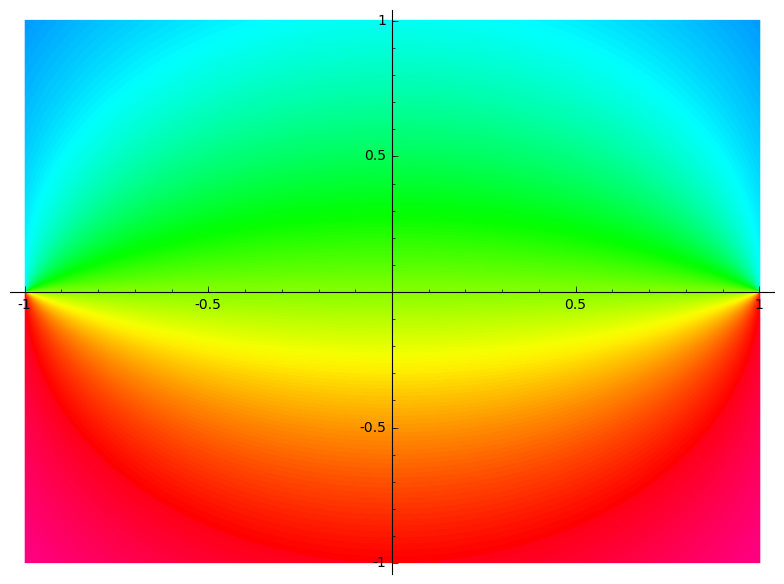
\includegraphics[width=0.8\linewidth]{graphics/sage0}
    \end{center}
    
    \paragraph{Παρ.} \hspace{0pt}
    
    \begin{tikzpicture}[scale=1.1]
    \fill[green!50,path fading=north] (-0.8,0) rectangle (0.8,2);
    
    \draw[->] (0,-0.1) -- (0,2)  node[midway,rotate=45] {$\nabla^2 \Phi = 0$};;
    \draw[->] (-2,0) -- (2,0);

    \draw[ultra thick, blue!50!cyan] (-0.8,0) -- (0.8,0) node[midway,below right,black]
    {$0$};
    \draw[ultra thick, blue!50!black] (-0.8,2) -- ++(0,-2) node[midway,left,black] {$5$};
    \draw[ultra thick, blue!70!black] (0.8,2) -- ++(0,-2) node[midway,right,black] {$10$};
    
    \draw[->] (2,1) to[bend left]  node[pos=.5,above] {$z=g(w)$} (3.8,1);
    \draw[->,gray!50] (3.8,0.8) to[bend right] (2,0.8);
    
    \begin{scope}[xshift=6cm]
    \fill[green!50] (-2,0) rectangle (2,0.7);
    \fill[green!50,path fading=north] (-2,0.7) rectangle (2,2);
    
    \draw (-2,0) -- (2,0);
    \draw[->] (0,-.1) -- (0,2);
    
    \draw (1,1) node {$\nabla^2 \Psi = 0$};
    
    \draw[very thick, blue!50!black] (-2,0) -- (-0.5,0)
    node[black,midway,below] {$5$};
    \draw[very thick, blue!50!cyan] (-0.5,0) -- (0.5,0)
    node[black,midway,below] {$0$};
    \draw[very thick, blue!70!black] (0.5,0) -- (2,0)
    node[black,midway,below] {$10$};
    \end{scope}
    \end{tikzpicture}
    \begin{align*}
    	w = f(z) &= \sin(\pi z) \\
    	z = g(z) &= \frac{1}{\pi} \arcsin(w)
    \end{align*}
    
    Υπενθυμίζουμε ότι
    \begin{align*}
    	w &= \sin(\phi) = \sin(a+ib) =
    	\\ &= \sin(a)\cos(ib)+\sin(ib)\cos(a)
    	\\ &= \sin a \cosh b +i\sinh b \cos a \\
    	w &= \sin(\pi z) = \sin(\pi x) \cosh(\pi y) +i\sinh(\pi y)\cos(\pi x)
    \end{align*}
    
    Και η λύση προκύπτει:
    \begin{align*}
    \Aboxed{
    	\Psi &= \frac{5}{\pi}\arctan(v,u+1) - \frac{10}{\pi} \arctan(v,u-1) + 10
    	} \\
    \Aboxed{
    	\Phi &= {\begin{array}{ll}
    	& \frac{5}{\pi}\arctan\left(
    	\sinh(\pi y)\cos(\pi x),\sin(\pi x)\cosh(\pi y) + 1
    	\right)
    	\\ - & \frac{10}{\pi}\arctan\left(
    	\sinh(\pi y)\cos(\pi x),\sin(\pi x)\cosh(\pi y) - 1
    	\right) \\ + & 10
    	\end{array}}
    }
    \end{align*}
    
    % Sage code:
    % var('x y')
    % psi(u,v) = 5/pi*arctan2(v,u+1) - 10/pi*arctan2(v,u-1) + 10
    % phi(x,y) = psi(sin(pi*x)*cosh(pi*y), sinh(pi*y)*cos(pi*x))
    % density_plot( phi(x,y), (-1,1), (0.1,1) , cmap = 'hsv', plot_points=1200)
    \begin{center}
    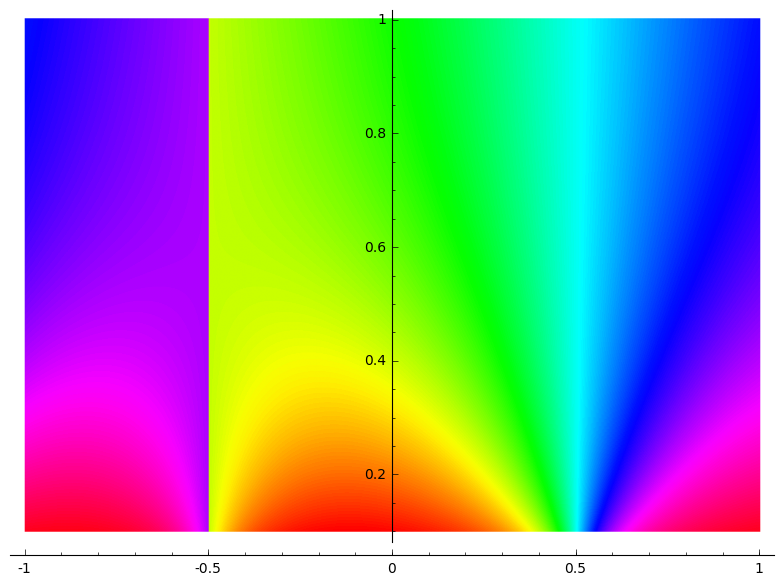
\includegraphics[width=0.8\linewidth]{graphics/sage1}
    \end{center}

\end{document}
